\documentclass{ctexart}

\usepackage{abstract}
\usepackage{CJKutf8}
\usepackage{geometry}
\usepackage{ctex}
\usepackage{color}
\usepackage{float}
\usepackage{soul}
\usepackage{amsmath}
\usepackage[british]{babel}
\usepackage[utf8]{inputenc}
\usepackage{epstopdf}
\usepackage{csquotes}
\usepackage[hidelinks]{hyperref}
\usepackage[T1]{fontenc}
\usepackage{enumitem}
\usepackage{caption} 
\usepackage{graphicx}  % Required for inserting images
\usepackage[
    style=apa,
    backend=biber,
    sortcites=true,
    sorting=nyt,
%    isbn=false,
%    url=false,
%    doi=false,
%    eprint=false,
    hyperref=false,
    backref=false,
%    firstinits=false,
]{biblatex}

\renewcommand{\abstractnamefont}{\Large\bfseries}

\newcommand{\enabstractname}{Abstract}
\newcommand{\cnabstractname}{\Large{摘要}}
\newenvironment{enabstract}{%
  \par\Large
  \noindent\mbox{}\hfill{\bfseries \enabstractname}\hfill\mbox{}\par
  \vskip 2.5ex}{\par\vskip 2.5ex}
\newenvironment{cnabstract}{%
  \par\large
  \noindent\mbox{}\hfill{\bfseries \cnabstractname}\hfill\mbox{}\par
  \vskip 2.5ex}{\par\vskip 2.5ex}


% section title format
\ctexset{
    section={
        name={,.},
        format+ = \raggedright, % 一级标题左对齐
        aftername = \hspace{4pt}
    },
    subsection={
        titleformat+ = \textit, % 标题内容斜体
        aftername = \hspace{2pt}
    },
    subsubsection={
        titleformat+ = \textit, % 标题内容斜体
        aftername = \hspace{2pt}
    },
}

% figure caption
\captionsetup[figure]{
    labelfont = {it}, % 斜体Figure
    labelsep = space, % 去掉冒号
}

% maps apacite commands to biblatex commands
\let \citeNP \cite
\let \citeA \textcite
\let \cite \parencite

\bibliography{reference}

% 1英寸边界
\geometry{a4paper, right=1in, left=1in, top=1in, bottom=1in} 

% 页码放下面
\pagestyle{plain} 

% 1.5行间距
\linespread{1.5} 

% title
\title{\LARGE{\bfseries{Syntactic Structure and Semantic Interpretation of Constructions on Gradable Adjectives in Mandarin}}}
\date{\vspace{-10ex}}

% enumerate列表格式
\setlist[enumerate,1]{
    resume,
    label=(\arabic*)
    }

\setlist[enumerate,2]{
    leftmargin=*,
    labelindent=16pt,
    label=(\alph*),
    ref=(\arabic{enumi}\alph*),
    }

%%%%%%%%%%%%%%%%%%%%%%%%%%%% 摘要 英文
\newpage

\begin{abstract}
    \normalsize 
    {

    This paper focuses on sentences built around gradable adjectives, especially measurable ones, used as predicates in Mandarin. These sentences are classified as expressing assignable meaning or comparative meaning according to the lexical entry of the gradable adjective. In terms of the latter type, sentences are further divided into three subtypes, i.e., positivity, superiority and equality. 

    The whole research is conducted under the theoretical frame of generative syntax and formal semantics. The paper attempts to give a complete analysis integrating syntax and semantics. DegP hypothesis and DegP-shell are the two main cornerstones of this research.

    For the syntactic part, this paper assumes a perspective of the complementary distribution of ``DegP-AP'' and ``DegP-DegP-AP'' structures. In detail, the higher DegP serving to introduce the standard is consistently projected, while the lower DegP severing to introduce the gap between the comparee and the standard is projected on the condition of the appearance of a differential phrase strictly greater than zero. 

    For the semantic part, this paper makes a clear division of labour among the gradable adjective, the lower functional degree head and the higher functional degree head. Thanks to this division, wrong readings of some constructions on gradable adjectives derived out via previous analyses are successfully corrected. Detailed semantic formalizations and calculations are illustrated with examples of different types of constructions built around gradable adjectives. 

    
    \vspace{2ex}
    \bf{ Keywords: gradable adjectives; degree; DegP}
    }
    
\end{abstract}

\thispagestyle{empty} % 这一页清空

%%%%%%%%%%%%%%%%%%%%%%%%%%%% 摘要 中文
\newpage

\begin{cnabstract}
    本文聚焦於研究漢語普通話當中有級形容詞作謂語的句子,其中對可度量有級形容詞的研究更是本文的重中之重。這些句子根據有級形容詞的語詞條目被分成兩類,一類表達賦值含義,另一類表達比較含義。而後者,又進一步被細分為三種子類,即,肯定義,差比義和等比義。

    全文的研究是以聲稱語法和形式語義為理論框架而展開的。本文旨在給出一個能夠融合句法和語義的全面完整的分析體系。DegP假設和DegP-壳是文研究的兩大基石。

    句法方面,本文提出一種“DegP-AP”和“DegP-DegP-AP”兩個結構呈互補分布的理論觀點。詳細來說,上層DegP永遠會投射,它的作用是引入比較標準;而下層DegP的投射則是以嚴格大雨零的差別短語之存在作為條件的,它的作用是引入比較對象和比較標準之間的差距。

    語義方面,本文對於有級形容詞,下層功能性程度中心語和上層功能性程度中心語的功能做出了明確的分工。這一分工,使得由從前的研究所做出的一些和有級形容詞有關的結構之錯誤語義被成功地修正過來。圍繞有級形容詞建立的不同類型結構被援引作本文當中的例子,詳細的語義形式化表達以及語義計算經由這些例子而呈現出來。

    \vspace{2ex}
    \bf{關鍵字: 有級形容詞;程度;DegP}

\end{cnabstract}

\thispagestyle{empty} % 这一页清空

%%%%%%%%%%%%%%%%%%%%%%%%%%%% 目录

\newpage

\tableofcontents

\thispagestyle{empty} % 这一页清空

%%%%%%%%%%%%%%%%%%%%%%%%%%%% 正文

\newpage

\section{INTRODUCTION}

\setcounter{page}{1}

\noindent
From traditional view, ingredients of a comparative construction are, a comparee, a standard, a comparative marker and a gradable predicate \cite{guo2012}. And from this paper's perspective, in semantics, a comparative construction can be departed to a comparee, a standard, a gradable predicate, and a optional differential phrase; in syntax, there are two more ingredient, comparative marker and comparative morpheme.

A simplest example in English is shown in \ref{degree_construction_example}. in this sentence, \textit{John} is comparee, \textit{Mary} is standard, suffix \textit{er} is a comparative morpheme whose job is introduce strict partial relation meaning ``greater than'', and word \textit{than} is another comparative marker whose function is still controversial. Some researchers believe that \textit{than} is just a word in specifier position without crucial function \cite{von1984a,heim1985,bhatt2004,rullmann1995}, another kind of view treats this word as a head of degree phrase (DegP) \cite{bierwisch1989,corver1990,corver1993,corver1997a,kennedy1997,grano2012}. Different form English, Mandarin is considered as a single mark language in comparative expression \cite{bobaljik2012,grano2012}. In most of cases, this mark is morpheme \textit{bi}(`than') such as example in \ref{degree_construction_example_Mandarin}, and there is no inflection of adjectives in Mandarin like \textit{er} in English \cite{guo2012}. 

\begin{enumerate}
    \item \label{degree_construction_example}
    John is taller than Mary.
\end{enumerate}

\begin{enumerate}
    \item \label{degree_construction_example_Mandarin}
    John \enspace bi \enspace Mary \enspace gao.  \\
    John than Mary \enspace tall. \\
    `John is taller than Mary.'
\end{enumerate}

Differential phrase (DiffP) is an important part of comparative structure, whose job is to give the gap between targets in comparison. A comparative structure with differential phrase in English is shown in \ref{degree_construction_dp_example}, and Mandarin version is shown in \ref{degree_construction_dp_example_Mandarin}.

\begin{enumerate}
    \item \label{degree_construction_dp_example}
    John is 2 meters taller than Mary.
\end{enumerate}

\begin{enumerate}
    \item \label{degree_construction_dp_example_Mandarin}
    John \enspace bi \enspace Mary \enspace gao \enspace 2 mi.  \\
    John than Mary \enspace tall 2 meters. \\
    `John is 2 meters taller than Mary.'
\end{enumerate}

The differential phrase in examples above are denoted by specific value, which gives an accurate value of scale about the gradable adjective. Another type of differential phrase gives vague value of scale. When this kind of differential phrase appears in comparative meaning, there is always a standard differential scale existing in context, and this vague value is either bigger than the standard differential value, or smaller than the standard differential value. Like example in \ref{dp_big_vague_example}, morpheme \textit{hen duo}(`much') is a big vague differential phrase, which means, John is not only taller than Mary, but also, the difference of their height is lager than a standard value. This standard value is given in context, it is a consensus between speakers. Similarly, a small vague differential phrase is shown in \ref{dp_small_vague_example}. In Mandarin, vague differential phrase can be complex, many researchers \cite{lin2014,li2015} do deeply investigation on it, \ref{dp_value_big_vague_example} and \ref{dp_value_small_vague_example} show such type of differential phrase which appears as ``vague prefix + accurately value'' or ``accurately + vague suffix''.

\begin{enumerate}
    \item
    \begin{enumerate}
        \item \label{dp_big_vague_example}
        John \enspace bi \enspace Mary \enspace gao \enspace hen duo.\\
        John than Mary \enspace tall \enspace \enspace much. \\
        `John is much taller than Mary.'

        \item \label{dp_small_vague_example}
        John \enspace bi \enspace Mary \enspace gao \enspace yi dian.\\
        John than Mary \enspace tall \enspace a little.\\
        `John is a little taller than Mary.'

    \end{enumerate}
\end{enumerate}

\begin{enumerate}
    \item
    \begin{enumerate}
        \item \label{dp_value_big_vague_example}
        John \enspace bi \enspace Mary \enspace gao \enspace liang mi \enspace \enspace duo.\\
        John than Mary \enspace tall \enspace 2 meters \enspace more. \\
        `John is more than 2 meters taller than Mary.'

        \item \label{dp_value_small_vague_example}
        John \enspace bi \enspace Mary \enspace gao \enspace bu.dao \enspace liang mi.\\
        John than Mary \enspace tall \enspace \enspace less \enspace \enspace \enspace 2 meters. \\
        `John is less than 2 meters taller than Mary.'
    \end{enumerate}
\end{enumerate}

In comparative structure built by gradable adjectives, sometimes, the standard is not a specific individual. This paper propose that there are three categories of standard, which are ``single individual standard'', ``individual set standard'' and ``specific value standard''. All examples mentioned above is single individual comparison. \ref{specific_value_comparison_example} gives an example of specific value comparison, in which standard is not a individual. \ref{individual_set_comparison_example} shows an example of individual set comparison.

\begin{enumerate}
    \item
    \begin{enumerate}
        \item \label{specific_value_comparison_example}
        John \enspace bi \enspace \enspace 2 mi \enspace \enspace \enspace gao.\\
        John than 2 meters \enspace tall. \\
        `John is taller than 2 meters.'

        \item \label{individual_set_comparison_example}
        zai \enspace yi.ban, \enspace John zui \enspace gao.\\
        in \enspace class.one, John most tall.\\
        `John is tallest in class one.'

    \end{enumerate}
\end{enumerate}

Then we propose a classification of degree structure into two types, assignable meaning and comparative meaning.

\begin{itemize}

    \item[1.] \textbf{Assignable meaning}: a degree structure is assignable meaning if and only if the function of gradable adjective is assignment. Under assignable meaning, there is no more subtypes, \ref{assignable_meaning_example} shows an example, where gradable adjective assigns a accurately value \textit{2 mi}(`2 meters') to another individual's height. When a scale-related group of words appears in assignable meaning, this paper do not call it differential phrase, but measure phrase (MP). Many researchers do not separate this two concepts very clear. Under our discussion, differential phrase appears in comparative meaning, measure phrase appears in assignable meaning. 
    
    \begin{enumerate}
        \item \label{assignable_meaning_example}
        John gao \enspace 2 mi.\\
        John tall 2 meters. \\
        `John is 2 meters tall.'
    \end{enumerate}
    
    \item[2.] \textbf{Comparative meaning}: a degree structure is comparative meaning if and only if the function of making comparison is encoded in the gradable adjectives. Under comparative meaning, there are three subtypes, positivity, superiority and equality. 
    
    \begin{itemize}

        \item[i.] \textbf{Comparative of positivity}: a degree structure is classified as positivity if and only if the standard is a consensus in people's mind which does not need to be indicated explicitly from the utterance or inferred implicitly from the context. \ref{positivity_example} gives an example of positivity, which tells a truth that, the value of John's height is greater than a standard degree existing in people's mind. 
        
        \begin{enumerate}
            \item \label{positivity_example}
            John hen gao. \\
            John very tall. \\
            `John is very tall.'
        \end{enumerate}
        
        \item[ii.] \textbf{Comparative of superiority}: a degree structure is classified as superiority if and only if the standard needs to be indicated explicitly from the utterance or inferred implicitly from the context and the difference between comparee and standard is strictly greater than zero. \ref{degree_construction_example_Mandarin} is an example of comparative of superiority, which is basic type of degree structure. What should be noticed is example in \ref{individual_set_comparison_example}, which also belongs to comparative meaning type and superiority subtype. This degree structure belongs to comparative meaning because the gradable adjective here still bears comparison job, which compares height between \textit{John} and an individual set. And the example is comparative of superiority on account of that this superlative expression gives a truth that the the value of \textit{John}'s height is greater than any of individual included in this set.
        
        \item[iii.] \textbf{Comparative of equality}: a degree structure is classified as equality if and only if the standard needs to be indicated explicitly from the utterance or inferred implicitly from the context and the difference between comparee and standard is equal to zero. \ref{equality_example} shows an example of comparative of equality, which gives an expression that the value of John's height is same with the value of \textit{Mary}'s height. Here may have some controversies, someone may think that, \ref{equality_example} actually assigns the value of \textit{Mary}'s height to \textit{John}'s height, which will lead the function of gradable adjective turn to assignment \cite{guo2012}. This paper argues that, the height is kind of inner property of an individual, so we can not assign one's height to another. On the opposite, the essence of equality is to express a truth that, the difference between two individuals height is zero, thus the function of gradable adjective in equative form is comparison rather than assignment.
        
        \begin{enumerate}
            \item \label{equality_example}
            John he \enspace Mary \enspace yi.yang \enspace gao.\\
            John and Mary \enspace \enspace same \enspace \enspace tall.\\
            `John is as tall as Mary.'
        \end{enumerate}

    \end{itemize}   

\end{itemize}

Up to now, it is time to summarize all kinds of classifications mentioned above. First of all, a degree structure built by gradable adjectives can be classified into two categories, comparative meaning and assignable meaning. If gradable adjectives bear value assignment function, sentences can be seen as expressing assignable meaning. If gradable adjectives bear comparison function, the degree structure can be seen as expressing comparative meaning. And in comparative meaning, sentences can be classified as positivity, superiority and equality. In superiority, there are three different angles to classify degree structures. 

\begin{itemize}
    \item[1.] The differential phrase is explicit or implicit.
    \item[2.] The standard is specific value or single individual or individual set.
    \item[3.] The standard is determined by the context or existing in people's mind.
\end{itemize}

For now, we have given a clear classification to degree structures, and in next sections, we are going to make a deeper discussion about the syntactic and semantic properties of those degree structures. In section 2, this paper will enumerate some former researchers' work about degree semantics. In section 3, some details about how gradable adjectives express assignable meaning will be explored. In section 4, this paper will unfold properties of sentences built around gradable adjectives which express comparative meaning, from the perspective of generative syntax and formal semantics respectively. Section 5 is a conclusion.

\section{FORMER DEGREE SEMANTICS RESEARCH}

\noindent
First founder of analysis on gradable adjectives is Cresswell \cite{cresswell1976}, who creates a third primitive semantic type $d$ besides the two primitive semantic types $e$ and $t$ in classical semantics Degree semanticists also identify three major parts of gradable adjectives:

\begin{itemize}
    \item[1.] A measure function $G$, mapping the target $x$ onto the abstract dimension for measurement characteristic of the gradable adjective \cite{bartsch1974}.
    \item[2.] The total ordering relation $\geq$, which makes the set of scales corresponding to the abstract dimension ordered in pairs of a same direction.
    \item[3.] The degree variable, indicating the value of $G(x)$. A gradable adjective of predictive use is analyzed as a two-place predicate with the individual and the degree as its arguments.
\end{itemize}

After this, lots of research of degree sematic are raised up in past decades. Generally, there are two directions to discuss degree semantics, a syntactic way and semantic way. In syntax, scholars talk about the syntactic structure of degree phrase(DegP) and adjective phrase(AP), and serval classical structure came up in years. In semantic, scholars discuss the lexical entry of gradable adjectives and other morphemes appeared in degree construction, make lexical calculation, and try to make the application of their definition as large as possible.

\subsection{Syntactic way}

\noindent
At the beginning, most researchers believe degree phrase is a specifier of adjective phrase \cite{chomsky1977,selkirk2015,bresnan1973,heim2000}, this kind of structure shows in \ref{old_deg_structure}. The main problem of this structure is that, standard as complement of the degree head will cause different degree heads lead different kinds of complements. In example \ref{old_deg_structure_example} shows this conflict, morpheme \textit{er} selects \textit{than Mary} as its complement, and \textit{est} selects \textit{all students} as its complement. But \textit{est} can not select \textit{than Mary}, which will cause grammar failure. The other problem of this kind of syntactic structure is that, a movement exists in this structure which makes gradable adjective moves from head of AP to AP's specifier phrase's head, aiming to combine with the degree head, shown in \ref{traditional_move}. This is not a acceptable movement.  

\begin{enumerate}
    \item \label{old_deg_structure} $[_{AP}[_{DegP}Deg[Standard]][_{A}...]]$
\end{enumerate}

\begin{enumerate}
    \item \label{old_deg_structure_example}
    \begin{enumerate}
        \item John is taller than Mary.
        \item John is tallest of all students.
    \end{enumerate}
\end{enumerate}

\begin{enumerate}
    \item \label{traditional_move}
\end{enumerate}

\begin{figure}[H]
    \centering
    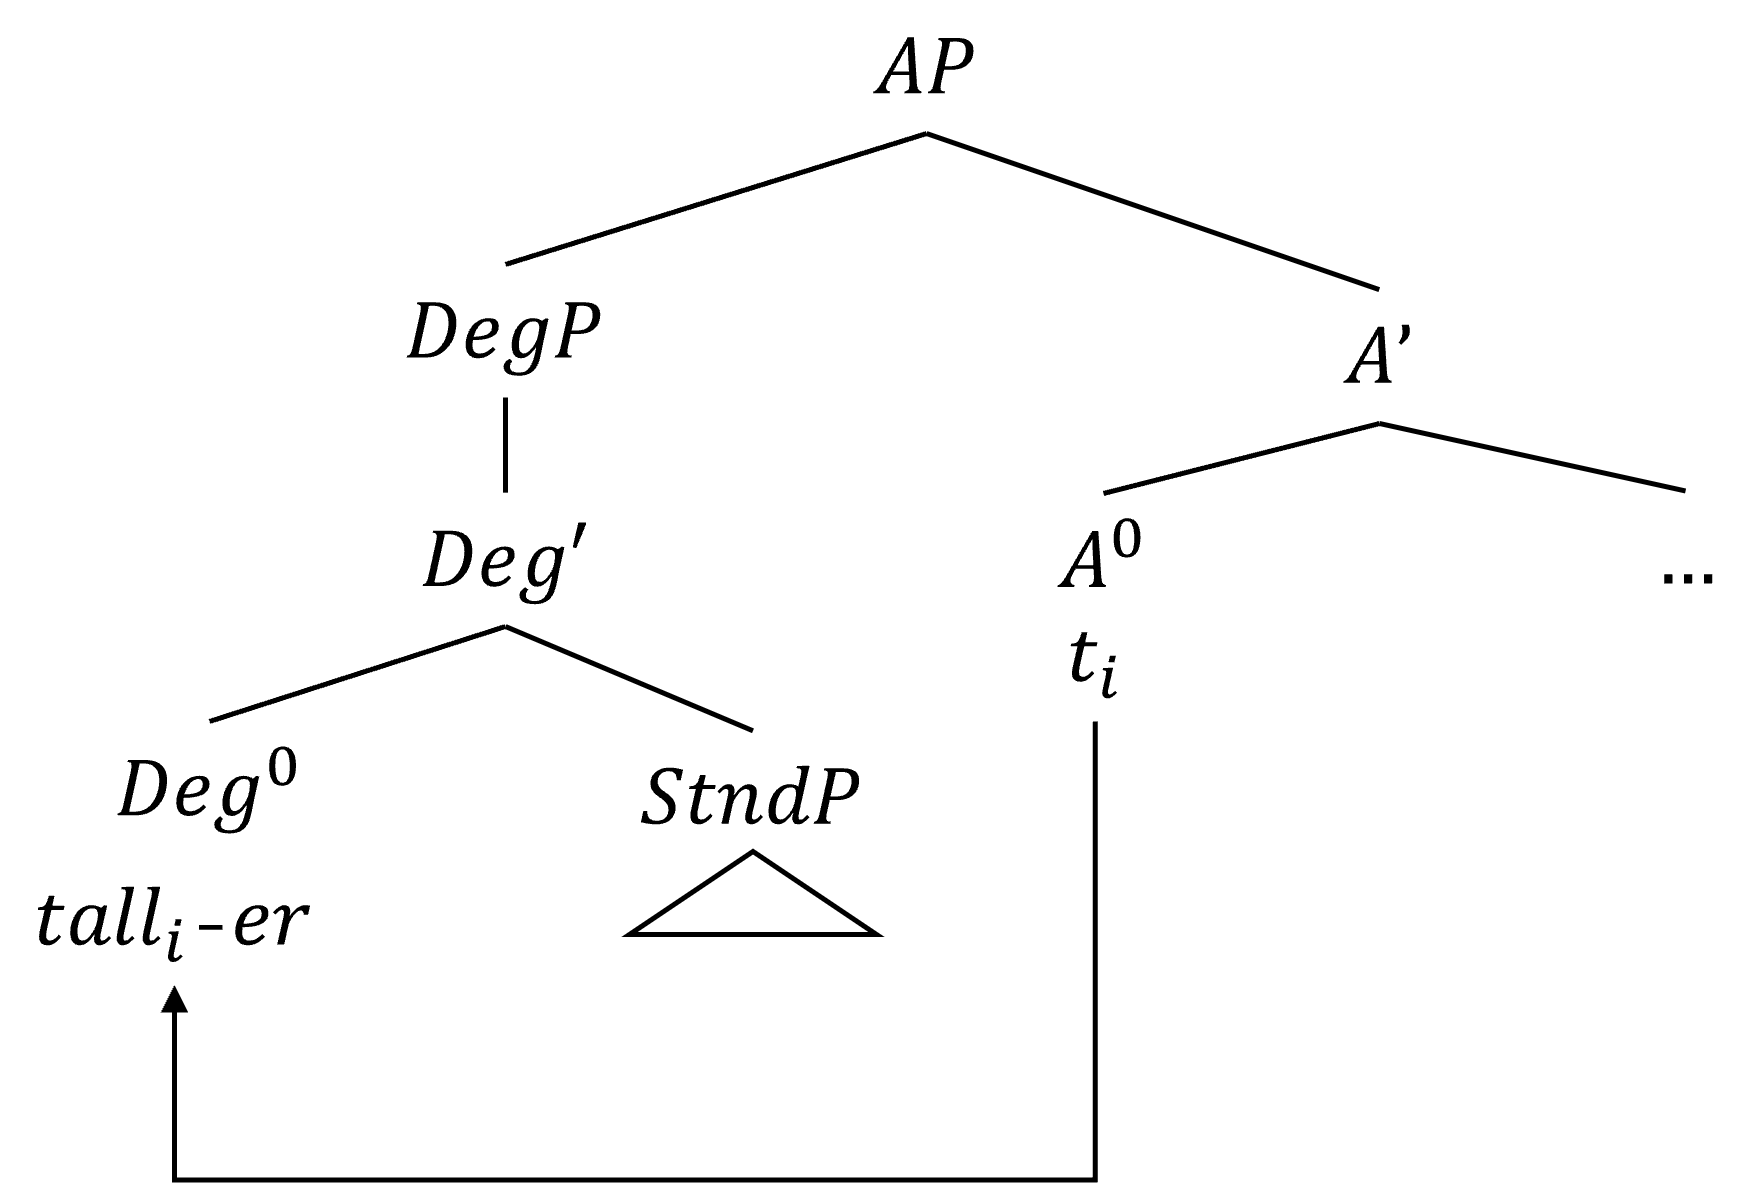
\includegraphics[width=0.4\textwidth]{Pic/traditional_move.png}
    \begin{caption}
        \\ \vspace{-1.1ex}
        Adjective movement when DegP as specifier of AP.
    \end{caption}
\end{figure}

Abney argues that degree phrase is a functional projection which is above the adjective phrase \cite{abney1987}, and a lot of researchers follow it \cite{corver1993,zwarts1992}. This structure treats DegP as a natural extended projection of the gradable adjectives \cite{grimshaw2005}, and as a functional projection, selecting AP as its complement. This theory is called DegP hypothesis by later scholars. In DegP hypothesis, the general structure is described as followed. The XP in \ref{abney_deg_p} is different in different situation, it may quantifier phrase, or differential phrase, or measure phrase. Three examples and their syntactic structures shown in \ref{abney_deg_p_example}.

\begin{enumerate}
    \item \label{abney_deg_p} $[_{DegP} XP [_{Deg^{\prime}}Deg^0[_{AP}...]]] $
\end{enumerate}

\begin{enumerate}
    \item \label{abney_deg_p_example}
    \begin{enumerate}
        \item \label{abney_deg_p_example_1}
        much too tall.\\
        $[_{DegP} [_{QP} much]] [_{Deg^{\prime}}Deg^0 \enspace too [_{AP}tall]] $
        \item \label{abney_deg_p_example_2}
        two meters as tall.\\
        $[_{DegP} [_{MP} two \enspace meters]] [_{Deg^{\prime}}Deg^0 \enspace as [_{AP}tall]] $
        \item \label{abney_deg_p_example_3}
        two meters taller.\\
        $[_{DegP} [_{DiffP} two \enspace meters]] [_{Deg^{\prime}}Deg^0 \enspace er [_{AP}tall]] $

    \end{enumerate}
\end{enumerate}

DegP hypothesis fixes the problems mentioned above. For the first problem, degree head's complement becomes AP, and the comparee become AP's specifier. For the second problem, form \ref{degp_hypothesis}, we can tell that the gradable adjective moves form AP's head to DegP's head. The head of DegP, giving the comparative morpheme \textit{er} as the typical one, takes a ``than phrase'' (thanP) as its complement and a differential phrase as its specifier. Depending on various categories of complement in thanP as well as the overt appearance, such as \textit{2 meters}, or covert appearance of differential phrase. \textit{er} has kinds of semantic variants. First, \textit{er} can take a direct degree expression, such as than \textit{2 meters}, which denotes a degree argument typed $d$. Second, a comparative clause, such as \textit{than Mary is tall}, which denotes a property of degree argument, typed $<d,t>$ because according to the view of Chomsky, the comparative clause \textit{than Mary is tall} owns a deep structure looking like ``\textit{than} $how_i$ \textit{Mary is} $t_i$ \textit{tall}'' which undergoes \textit{wh}-movement, leaving the trace $t_i$ denoting a degree variable bound by $\lambda$-operator \cite{chomsky1977}. Third, a bare NP, such as \textit{than Mary}, regarded as a deletion from the full comparative clause \textit{than Mary is tall}, also denotes a property of degree argument typed $<d,t>$. Examples illustrated in \ref{er_var_example} are possible semantic variants of \textit{er}.

\begin{enumerate}
    \item \label{degp_hypothesis}
\end{enumerate}

\begin{figure}[H]
    \centering
    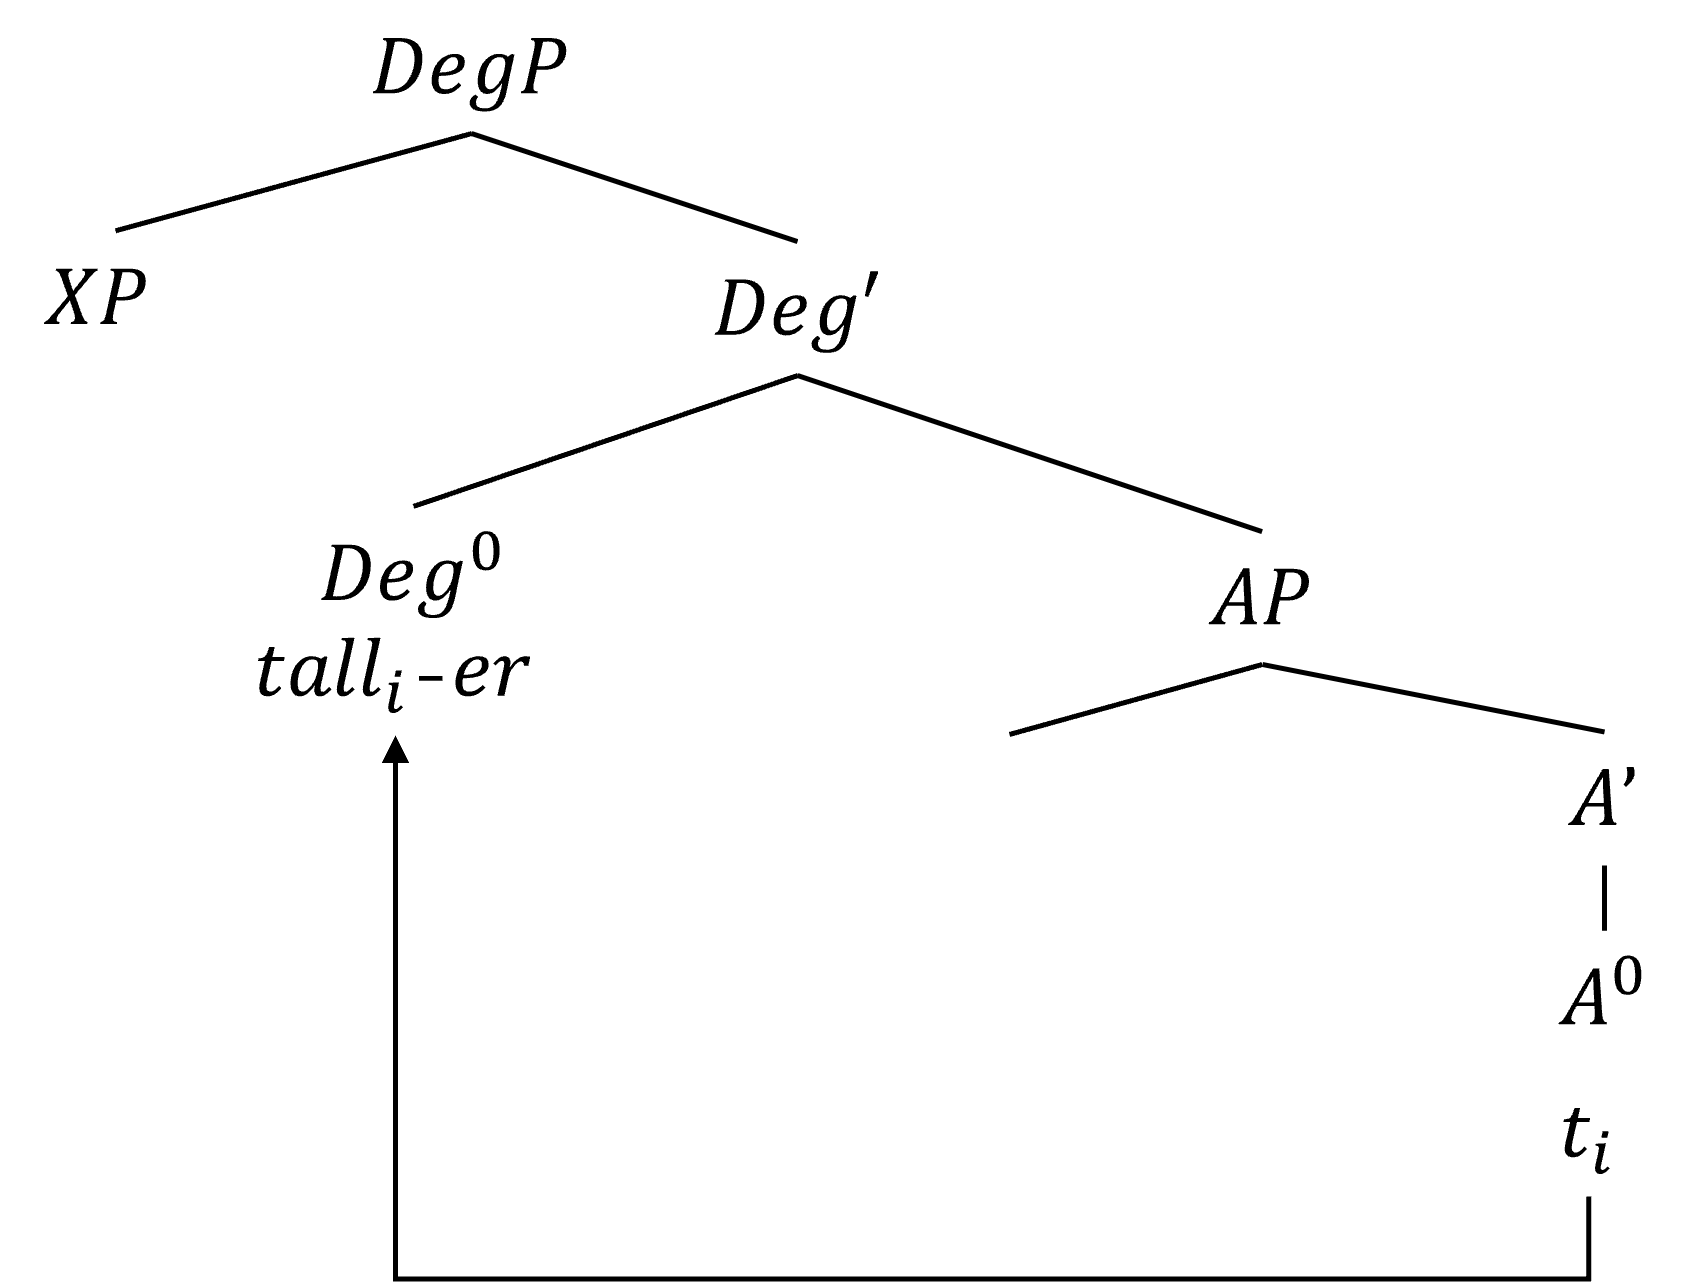
\includegraphics[width=0.35\textwidth]{Pic/degP_hy.png}
    \begin{caption}
        \\ \vspace{-1.1ex}
        Adjective movement in DegP hypothesis.
    \end{caption}
\end{figure}

\begin{enumerate}
    \item \label{er_var_example}
    \begin{enumerate}
        \item \label{er_var_1} John is taller than 6 feet.
        \item \label{er_var_2} John is taller than Mary.
        \item \label{er_var_3} John is taller than Mary is.
        \item \label{er_var_4} John is 6 inches taller than Mary is.
    \end{enumerate}

\end{enumerate}

After basic DegP hypothesis, there are serval modified versions raised up by later researchers. The most important modification of DegP hypothesis is the Larson's two layers DegP-shell structure \cite{larson1991}, and this kind of two layers shelled structure is the most famous structure in degree semantic these years \cite{grano2012,guo2012,xiang2005,fabregas2020}. In Larson's research, he propose a DegP-shell based on VP-shell structure, which is shown in \ref{deg_p_shell}. 

\begin{enumerate}
    \item \label{deg_p_shell} $[_{DegP} [_{Deg^{\prime}} Deg^0 [_{DegP} AP [_{Deg^{\prime}} Deg^0 [_{PP}...]]]]] $
\end{enumerate}

In this structure, the specifier of higher DegP is empty position, whose only job is to introduce lower DegP's head. So there are two movements need to be done. \ref{larson_structure} gives a movement structure of \textit{taller than Mary}. The first movement is comparative morpheme \textit{er} moving form lower DegP's head to higher DegP's head, where is empty position in original, second movement is gradable adjective moving form lower DegP's specifier to higher DegP's head, to combine with comparative morpheme \textit{er} moved here before.

\begin{enumerate}
    \item \label{larson_structure}
\end{enumerate}

\begin{figure}[H]
    \centering
    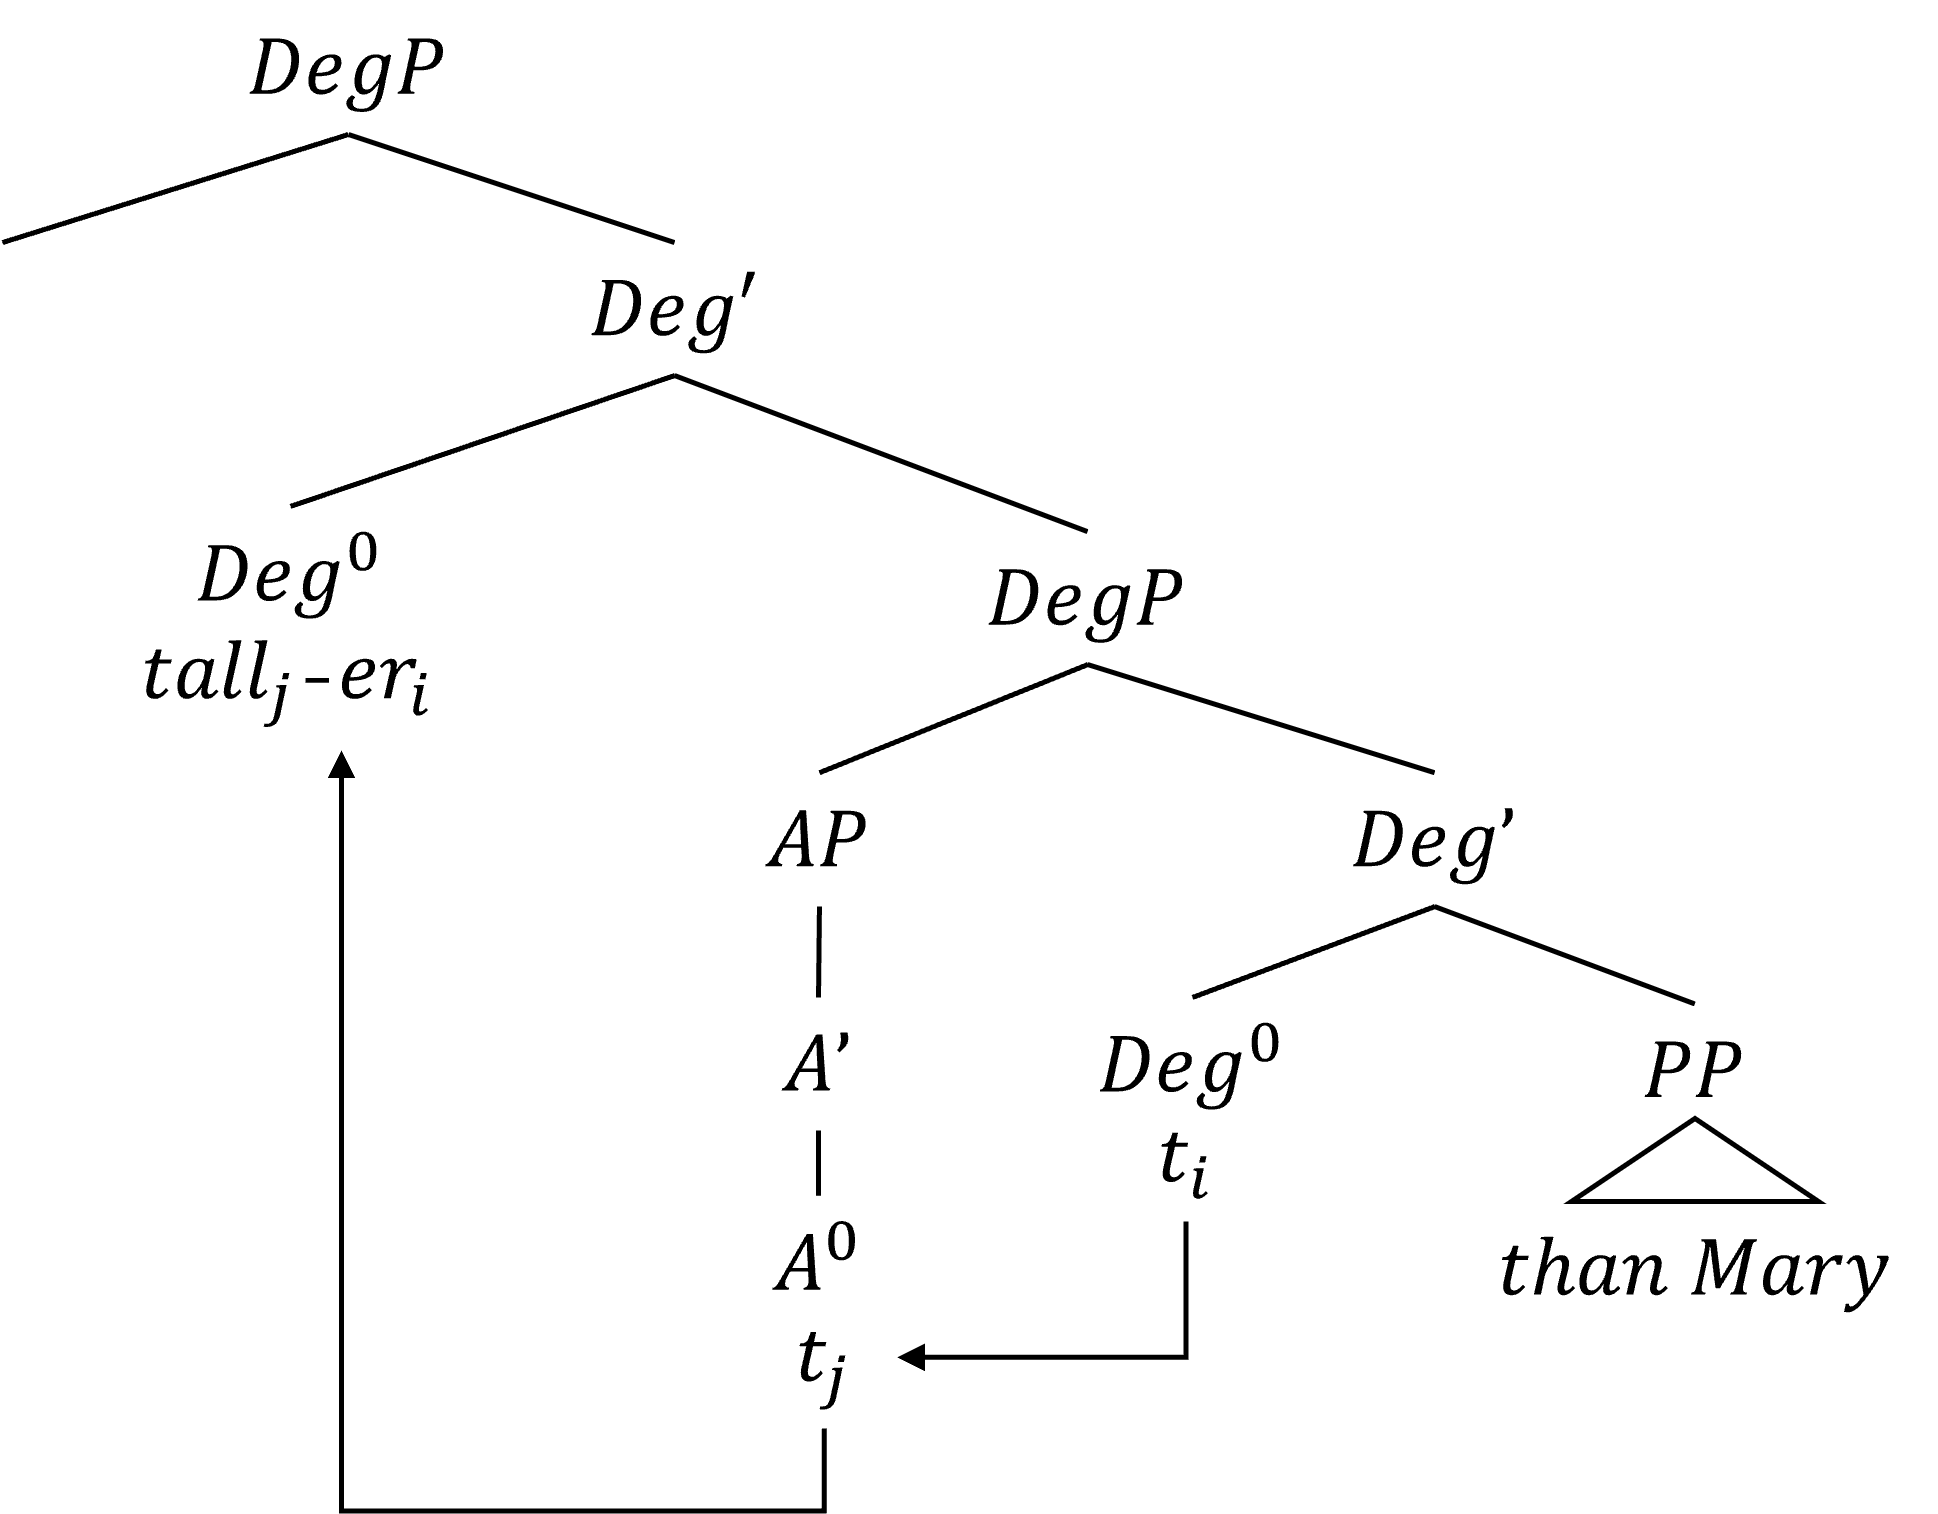
\includegraphics[width=0.45\textwidth]{Pic/larson1.png}
    \begin{caption}
        \\ \vspace{-1.1ex}
        Movements in Larson's DegP-shell structure.
    \end{caption}
\end{figure}

In Mandarin degree semantic, Xiang gives his structure with AP as higher DegP's complement and lower DegP as AP's complement. Structure's layout is shown in \ref{xiang_structure} explaining the movement of \ref{xiang_structure_example}, illustrates that AP is sandwiched by two DegPs \cite{xiang2005}. This structure is adopted by Grano who does little adjustment to explain transitive degree structure in Mandarin \cite{grano2012}. 

\begin{enumerate}
    \item \label{xiang_structure_example}
    John bi Mary gao chu 2 limi.  \\
    John than Mary tall exceed 2 centimeters. \\
    `John is 2 centimeters taller than Mary.'
\end{enumerate}

\begin{enumerate}
    \item \label{xiang_structure}
\end{enumerate}

\begin{figure}[H]
    \centering
    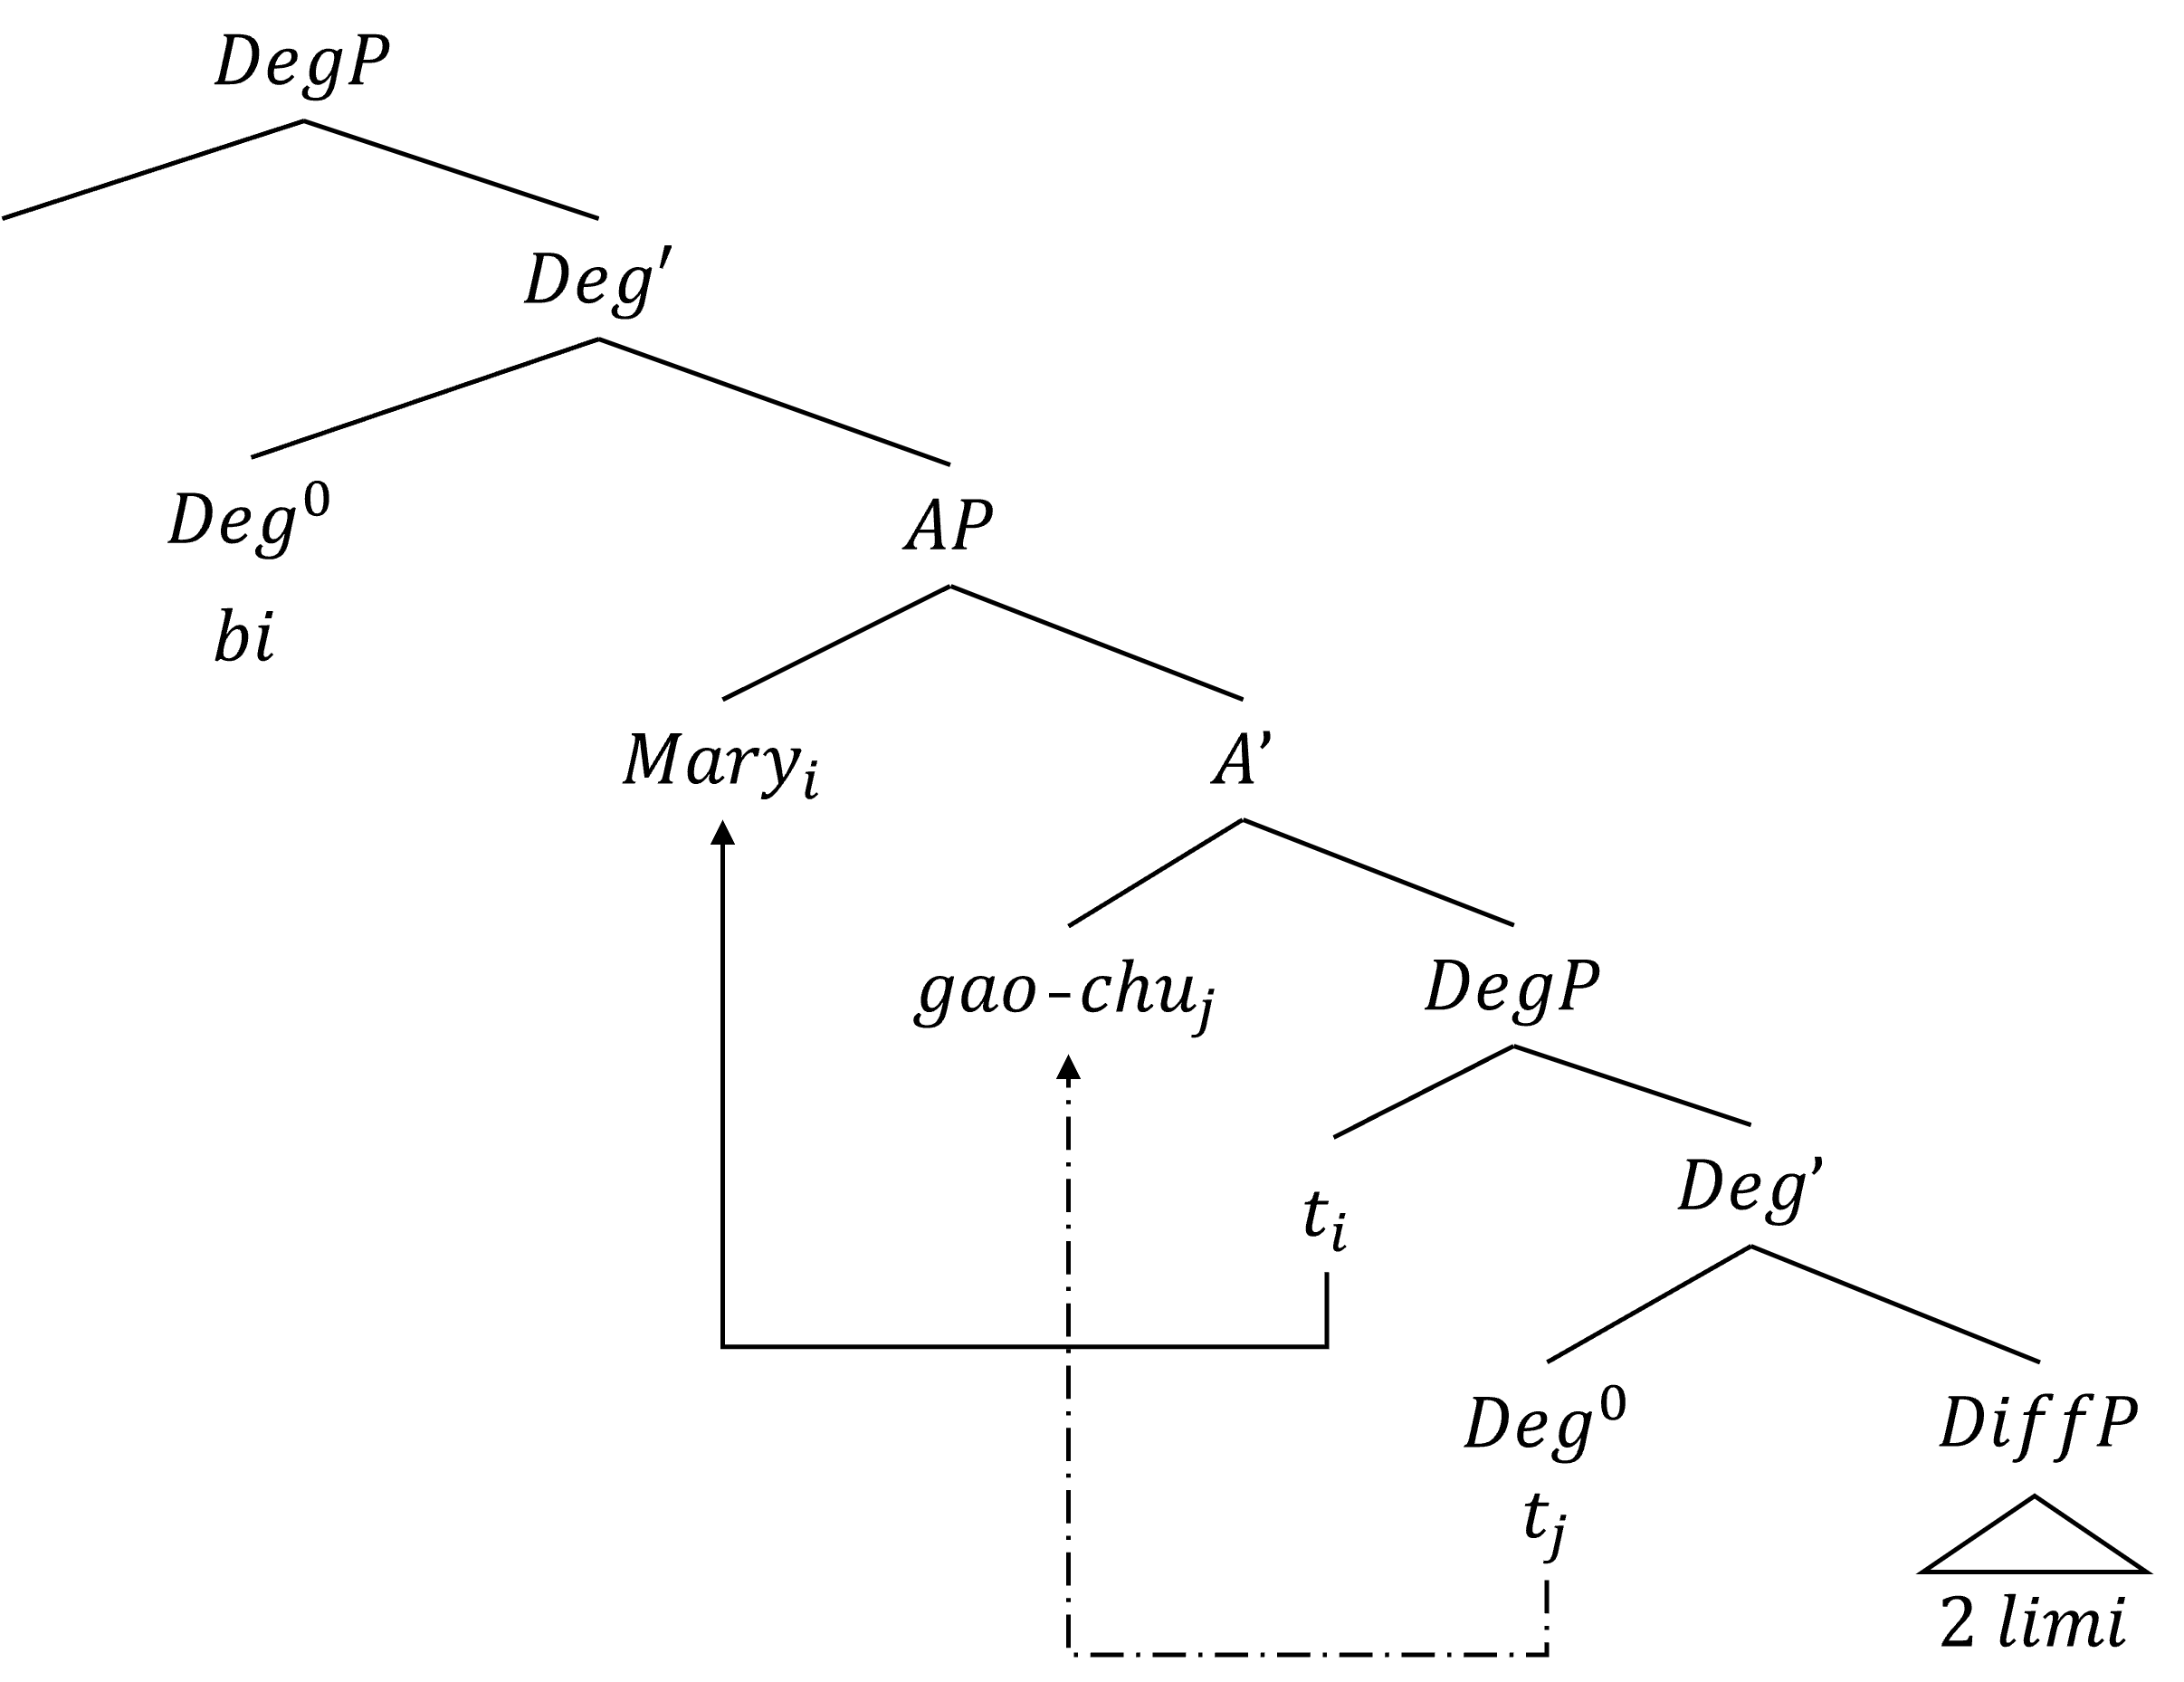
\includegraphics[width=0.55\textwidth]{Pic/xiang.png}
    \begin{caption}
        \\ \vspace{-1.1ex}
        Movements in Xiang's DegP-shell structure.
    \end{caption}
\end{figure}


\subsection{Semantic way}

\noindent
The definition of lexical entry of gradable adjectives is literally important, because different definitions of adjectives' lexical entry always lead totally different results in semantics and syntax just like butterfly effect. Since Cresswell, the semantic type of gradable adjectives is largely debated. Von Stechow proposes a comprehensive constructive analysis of comparisons \cite{von1984a}, which becomes the so-called standard analysis later \cite{bale2011}. From his view, the meaning of gradable adjectives are interpreted as a measure function and an ordering relation. The measure function maps the individual to the dimension denoted by gradable adjectives and the ordering relation ensures that the scale of the individual exceeds the degree to compare. In generative grammar, a gradable adjective is the head of adjective phrase. It functions as a two-place predicate, with an individual typed $e$ and a degree typed $d$ as its two arguments. What deserves a note is it is von Stechow who in first seriously regards degrees denoted by symbol $d$ as one of the primitive semantic types and it is degree $d$ that captures the difference between gradable adjectives and non-gradable adjectives. Here the semantic type of gradable adjectives is manifested as $<d,<e,t>>$. Still giving \textit{tall} as an instance, the lexical entry of a gradable adjective is shown in \ref{von_stechow_LE}, in which height denotes the measure function encoded by \textit{tall} and $\geq$ denotes the ordering relation between the individual and the degree:

\begin{enumerate}
    \item \label{von_stechow_LE} $[\![tall]\!] = \lambda d \lambda x. [height(x) \geq d]$
\end{enumerate}

The analysis of DegP headed by a degree morpheme is much more complicated. The semantic type of DegP is $<d,<e,t>>$. Based on the approach in generative grammar, DegP lands at an adjunct position of AP in the deep structure and then undergoes quantifier raising in the logical form to a node above the original IP inside which DegP is initially located, with the trace left denoting a $d$ type argument. The motivation for this movement is that, according to von Stechow's analysis, DegP can be regarded as isomorphic to a generated quantifier phrase, an account under large debate afterwards.

According to type-driven computation in formal semantics, the gradable adjective typed $<d,<e,t>>$ first combines the trace of the semantic type $d$ which is left by DegP in the process of QR, then combines the subject in the matrix clause of the semantic type $e$, outputting a $t$ type proposition with a free degree variable. $\lambda$-abstraction turns this $t$ type open proposition into a property of degree typed $<d,t>$ which saturates DegP typed $<<d,t>,t>$. Finally, a $t$ type proposition is made out. And this is the procedure in von Stechow's analysis of how to derive a comparative construction.

Base on $<d,<e,t>>$ type gradable adjective and syntactic structure mentioned above, we can give the lexical entries in \ref{er_var_example}. The thanP takes a direct degree expression as complement in \ref{er_var_1}, a bare NP in \ref{er_var_2}, a comparative clause in \ref{er_var_3} and \ref{er_var_4}. Optional differential phrase only owns overt appearance in \ref{er_var_4}. Based on the analysis above, sematic type of \textit{er} in \ref{er_var_1} is $<d,<<d,t>,t>>$, in \ref{er_var_2} as well as \ref{er_var_3} is $<<d,t>,<<d,t>,t>>$, in \ref{er_var_4} is $<<d,t>,<d,<<d,t>,t>>>$.

Under this definition, gradable adjective \textit{tall} is considered as a relation of ``greater equal'', which is true when an individual $x$ as input and $x$'s height is at least as great as $d$. A simple application of this kind of lexical entry definition to \ref{old_school_def_example} is shown in \ref{old_school_def_example_LE}.

\begin{enumerate}
    \item \label{old_school_def_example} 2 meters tall.
\end{enumerate}

\begin{enumerate}
    \item \label{old_school_def_example_LE}
    \begin{enumerate}
        \item $[\![tall]\!]=\lambda d \lambda x.[Height(x) \geq d]$
        \item $[\![2 \enspace meters \enspace tall]\!]=\lambda x.[Height(x) \geq 2 \enspace meters]$
    \end{enumerate}
\end{enumerate}

Actually, lexical entry definition like \ref{von_stechow_LE} remains a problem with corresponding examples shown in \ref{old_school_def_problem}. In English, sometimes measure phrase can not directly combine with negative-pole adjectives. We can say someone is \textit{2 meters tall}, but can not say someone is \textit{2 meters short}. But situation changes when suffix \textit{er} shows up in \ref{old_school_def_problem_correct}, \textit{2 meters shorter} is a correct usage in English. Besides, this phenomenon is also a language-specific problem, in Japanese, we can not combine measure phrase even with \textit{segatakai}(`tall'). Traditional lexical entry of gradable adjectives has no ability to explain this phenomenon.

\begin{enumerate}

    \item \label{old_school_def_problem}
    
    \begin{enumerate}
        
        \item 2 meters tall. 10 years old.
        \item *2 meters short. *10 years young.
        \item \label{old_school_def_problem_correct} 2 meters shorter. 10 years younger.

    \end{enumerate}

\end{enumerate}

Based on the problem mentioned above, there is another group of researchers propose that the gradable adjectives' lexical entry should not encode the partial ordering relation, instead, the gradable adjectives should reveal the original property of an individual, which means \textit{tall} should simply illustrate the height of an individual. Thus the lexical entry of gradable adjectives should looks like \ref{tallLE_b}, in which there is just a measure function. 

\begin{enumerate}
    \item \label{tallLE_b} 
    $[\![tall]\!]=Height(x)=d$
\end{enumerate}

Under this assumption, the partial ordering relation still needs a place to be introduced, if not, there will be a lexical entry type mismatch. The type of measure function \textit{tall} is $<e,d>$, but measure phrase is type $d$, so gradable adjectives are no way to composite with measure phrase on account of type-theoretic. To resolve this problem, Svenonius \cite{svenonius2006} claims that there is a null operator whose semantic function is linking the lexical entry of gradable adjectives and the lexical entry of measure phrase, and syntactic function is to introduce a degree argument and bear the mission of introducing the ``greater equal'' meaning. The denotation of this null operator is spelled out in \ref{gao_nop_LE}, and the \ref{gao_nop_LE_c} shows the composition of null operator and gradable adjective, which is same with \ref{von_stechow_LE}. The lexical entry of \ref{gao_nop_LE_c} is $<d,<e,t>>$, which can combine with measure phrase with out any type conflict.

\begin{enumerate}
    \item \label{gao_nop_LE}

    \begin{enumerate}
        \item \label{gao_nop_LE_a} 
        $[\![nop]\!]=\lambda G_{<e,d>}\lambda d \lambda x.[G(x) \geq d]$

        \item \label{gao_nop_LE_b} 
        $[\![tall]\!]=Height(x)$

        \item \label{gao_nop_LE_c} 
        $\begin{aligned}[t]
            [\![nop \enspace tall]\!] &= [\![nop]\!]([\![tall]\!]) \\
            &= \lambda d \lambda x.[Height(x) \geq d]
        \end{aligned}$

    \end{enumerate}
\end{enumerate}

Although the lexical result of null operator and adjectives in \ref{gao_nop_LE_c} looks exactly same with traditional lexical entry of gradable adjectives in \ref{von_stechow_LE}, which makes this null operator seems redundant. But this ``null operator + gradable adjective'' structure resolve the problem mentioned in \ref{old_school_def_problem}. Actually, this design separates the ``individual property function'' from ``greater equal meaning'', the former's owner is gradable function, and latter's owner is null operator. It is null operator who does not select for \textit{short} when measure phrase is \textit{2 meters}. And, this idiosyncratic property of null operator is language-specific. The advantage of this kind of structure is leaving language-specific problem to null operator and keeping gradable adjectives away form any idiosyncratic language-specific properties.

Next questions are, whether this null operator has a specific phonetic expression in any language and where its position is in syntactic structure. 

For the first question, Svenonius does a deep investigation about Icelandic and Norwegian, which shows that a phonetic word of this null operator does not exist in Norwegian but does exist in Icelandic. In Icelandic, \ref{Icelandic_example} gives three different ways to express the same meaning. In \ref{Icelandic_example_10}, the word \textit{Hversu} is mapping to two English words \textit{how.much}, but actually \textit{Hversu} only used as a degree operator, and it does not bear the function of manner adverbial. In \ref{Icelandic_example_a}, speaker can omit word \textit{Hversu} and front the predicate to express the same meaning. Also, in \ref{Icelandic_example_b}, a word \textit{Hvað} can be placed at the beginning of the sentence, and keep all other morphemes in their original position. What should be noticed is that the Icelandic word \textit{Hvað} does not have real meaning, it is just a phonologically placeholder, which exactly is an evidence of the existence of null operator. For the latter question, Svenonius gives syntactic structures of \ref{Icelandic_example} respectively as shown in \ref{Icelandic_example_LE}. From Svenonius' perspective, null operator and the word \textit{Hvað} show the same locality conditions which is same with famous \textit{wh}-movement. 

\begin{enumerate}
    \item \label{Icelandic_example}
    
    \begin{enumerate}
        \item \label{Icelandic_example_10}
        Hversu \enspace \enspace gammall \enspace ertu? \\
        how.much \enspace old \enspace \enspace \enspace are.you \\
        `how old are you?'

        \item \label{Icelandic_example_a}
        er \enspace du gammel? \\
        are you \enspace old \\
        `how old are you?'

        \item \label{Icelandic_example_b}
        Hvað ertu \enspace \enspace gammall? \\
        null \enspace are you \enspace old \\
        `how old are you?'

    \end{enumerate}   
    
\end{enumerate}

\begin{enumerate}
    \item \label{Icelandic_example_LE}
    
    \begin{enumerate}
        \item $[_{CP}Nop_1 \enspace er_2[_{IP}du_3 \enspace t_2[_{VP} t_2[_{AP} t_3 \enspace t_1 \enspace gammel]]]]$
        
        \item $[_{CP}Hva$ð$_1 \enspace er_2[_{IP} \enspace -tu_3 \enspace t_2 [_{VP}t_2[_{AP}t_3 \enspace t_1 \enspace gammel]]]]$
        
    \end{enumerate}   
    
\end{enumerate}

The $<e,d>$ type gradable adjectives seems a perfect definition. But I have to point out that, both lexical entries in \ref{von_stechow_LE} and \ref{tallLE_b} may cause a mismatch between the meaning given by lexical calculation and meaning given by language common sense. 

Since there are serval kinds of constructions of degree structures mentioned in first section which are comparative meaning and assignable meaning, a lexical should have ability to give a interpretation of all these structures. \ref{john_gao_2_mi} gives a assignable meaning form example, and it's lexical entry calculation is shown in \ref{john_gao_2_mi_LE}, who uses traditional gradable adjectives lexical type in \ref{von_stechow_LE}. To resolve $\lambda$ reduction, the lexical entry of \textit{tall} needs a measure phrase with lexical entry $d$ and an individual $x$ , which are respectively \textit{2 meters} and \textit{John}. \textit{2 meters} changes the semantic type of \textit{tall} from $<d,<e,t>>$ to $<e,t>$, and \textit{John} is input as type $e$ which makes final result to type $t$. The result of lexical entry calculation tells a truth that John's height is not only equal to 2 meters precisely, but also has a possibility to greater than 2 meters. But actually we do know that sentence in \ref{john_gao_2_mi} means John's height is 2 meters accurately, which is mismatch with the result of semantic calculation. The reason why this mistake is made is that the partial ordering relation of degree is encoded in gradable adjectives, and there is no way to resolve this ``greater equal''. \ref{tallLE_b} will also lead this problem, since the lexical entry of the combination of null operator and gradable adjective is same with the lexical entry shown in \ref{von_stechow_LE}.

\begin{enumerate}
    \item \label{john_gao_2_mi} Jhon is 2 meters tall.
\end{enumerate}

\begin{enumerate}
    \item \label{john_gao_2_mi_LE}
    
    \begin{enumerate}
    \item \label{john_gao_2_mi_LE_a} 
    $[\![tall]\!] = \lambda d \lambda x.[Height(x) \geq d]$
    
    \item \label{john_gao_2_mi_LE_b} 
    $\begin{aligned}[t]
        [\![2 \enspace meters \enspace tall]\!] &= [\![tall]\!](2m) \\
        &= \lambda x.[Height(x) \geq 2m]
    \end{aligned}$
    
    \item \label{john_gao_2_mi_LE_c} 
    $\begin{aligned}[t]
        [\![John \enspace is \enspace 2 \enspace meters \enspace tall]\!] &= [\![tall \enspace 2m]\!](John) \\
        &= Height(John) \geq 2m
    \end{aligned}$
    
    \end{enumerate}
\end{enumerate}

To fix this problem, this paper propose that the lexical entries of gradable adjective in superiority meaning and assignable meaning should be different. The detail will be discussed in next sections.

\subsection{Layout}

\noindent
This paper will do serval work to give semantic and syntactic analyses of constructions built around gradable adjectives (especially measurable gradable adjectives) in Mandarin. At the first, based on former researchers' work, this paper will give the lexical entry of gradable adjectives. After that, based on the classification given in the introduction, this paper will respectively give the analyses of different analyses.

From this paper's view, different meaning of degree constructions should have different lexical entries of gradable adjectives. Because the function of gradable adjectives is totally different in superiority meaning and assignable meaning. As discussed in introduction, a degree structure is superiority meaning when gradable adjective bears comparison function, so this paper adopt the partial ordering definition of lexical entry, which is re-wrote in \ref{tallLE_re_a}; and on the opposite, a degree structure is assignable meaning when gradable adjective bears assignment function, thus the lexical entry of gradable adjective should have a equal sign, which is shown in \ref{tallLE_re_b}.

Another reason which supports the separation of lexical entries is the mistake mentioned in last section. If a positive form has ``greater than'' meaning in gradable adjective, a wrong result will be calculated which makes \textit{John is 2 meters tall} expresses \textit{John is more than 2 meters tall}.

\begin{enumerate}
    \item \label{tallLE_re}
    
    \begin{enumerate}
        \item \label{tallLE_re_a} 
        $[\![tall]\!]=\lambda d \lambda x.[Height(x) \geq d]$
    
        \item \label{tallLE_re_b} 
        $[\![tall]\!]=\lambda d \lambda x.[Height(x) = d]$
    
    \end{enumerate}
\end{enumerate}

Next, follow the classification given in the introduction, the syntactic structure and semantic calculation will be given respectively in follow parts.

\noindent
At the beginning, here we propose that there are two types of syntactic structures in comparative meaning. For convenient, we give the two-layer-structure a name ``DegP-AP'' structure, and the three-layer-structure a name ``DegP-DegP-AP''. 

Generally speaking, the head of the higher DegP functions to introduce the standard, and the head of the lower DegP functions to introduce the difference between the degree of the comparee and the degree of the standard along the dimension of scale denoted by the gradable adjective. The gradable adjective is the head of the adjective phrase. From our intuition, the non-appearance of a standard (explicit or implicit) leads to the failure of expressing the comparative meaning. However, the difference between the comparee and the standard should in no way be expressed consistently. The occurrence of the difference between two objects naturally requires the the occurrence of the two objects to be compared as a prerequisite.For the semantic part, given the DegP hypothesis illustrated above, the higher DegP is obligatory in that, the extra argument $d$ should be bound by a functional projection which shifts the semantic type of gradable adjectives from $<d,<e,t>>$ to $<e,t>$, in order to absorb the comparee typed $e$ successfully. The differential phrase is not required by the lexical entry of gradable adjectives, which can also support its optional appearance. Here we assume that the lower DegP is projected if and only if there is an overt differential phrase and the differential phrase is strictly greater than zero. The non-appearance of a projection when it is not needed in completing the meaning of an utterance also satisfies the economical principal of language. And the explanations of this assumption will be elaborated immediately on the below.

In the following subsections, we further classifies the comparative meaning into three distinct subtypes, which are positivity, superiority and equality. We will unfold the syntactic structures and the semantic interpretations of these three subtypes below one by one.

\section{ASSIGNABLE MEANING}

\noindent
In assignable meaning degree Structure, this paper will adjust the standard lexical entry of gradable adjectives, modify the greater equal sign to absolute equal sign, which is shown in \ref{tallLE_re_b} and re-wrote in \ref{tallLE_re_re_b}. Because the gradable adjectives in assignable meaning bear the function of assignment, which is different with comparative meaning. If in assignable meaning with ``greater equal'' relation lexical entry, a mistake discussed in second 2 will occur, and the reason is the result of lexical entry calculation will be different with the original meaning. 

\begin{enumerate}
    \item \label{tallLE_re_re_b}
    $[\![tall]\!]=\lambda d \lambda x.[Height(x) = d]$
\end{enumerate}

\begin{enumerate}
    \item \label{assignable_example_1}
    \begin{enumerate}
        \item \label{assignable_example_1_a}
        John you \enspace 2 mi \enspace \enspace \enspace gao. \\
        John have 2 meters tall. \\
        `John is 2 meters tall.'
        
        \item \label{assignable_example_1_b}
        John you \enspace 2 mi \enspace \enspace duo \enspace gao. \\
        John have 2 meters more tall. \\
        `John is more than 2 meters tall.'
        
    \end{enumerate}
\end{enumerate}

Examples shown in \ref{assignable_example_1} are classical expression in assignable meaning, and the syntactic tree of \ref{assignable_example_1_a} is shown in \ref{assignable_structure}. The structure is quite similar with the syntactic structure of the comparative of superiority without DiffP shown in \ref{superiority_structure}. Little differences are, the morpheme \textit{you}(`have') take the place of the specifier of PredP, the measure phrase here we call it assignment phrase (assignP), and the operator at the head of DegP we call it $\varphi$. The movements in this tree are also similar with the movements in \ref{superiority_structure}, so there is need to repeat it.

\begin{enumerate}
    \item \label{assignable_structure}
    $[_{IP} NP [_{I'} I_0[_{...}[_{PredP}[_{Pred'}Pred^0[_{DegP}assignP[_{Deg'}Deg^0[_{AP}[A^0]]]]]]]]]$
\end{enumerate}

\begin{figure}[H]
    \centering
    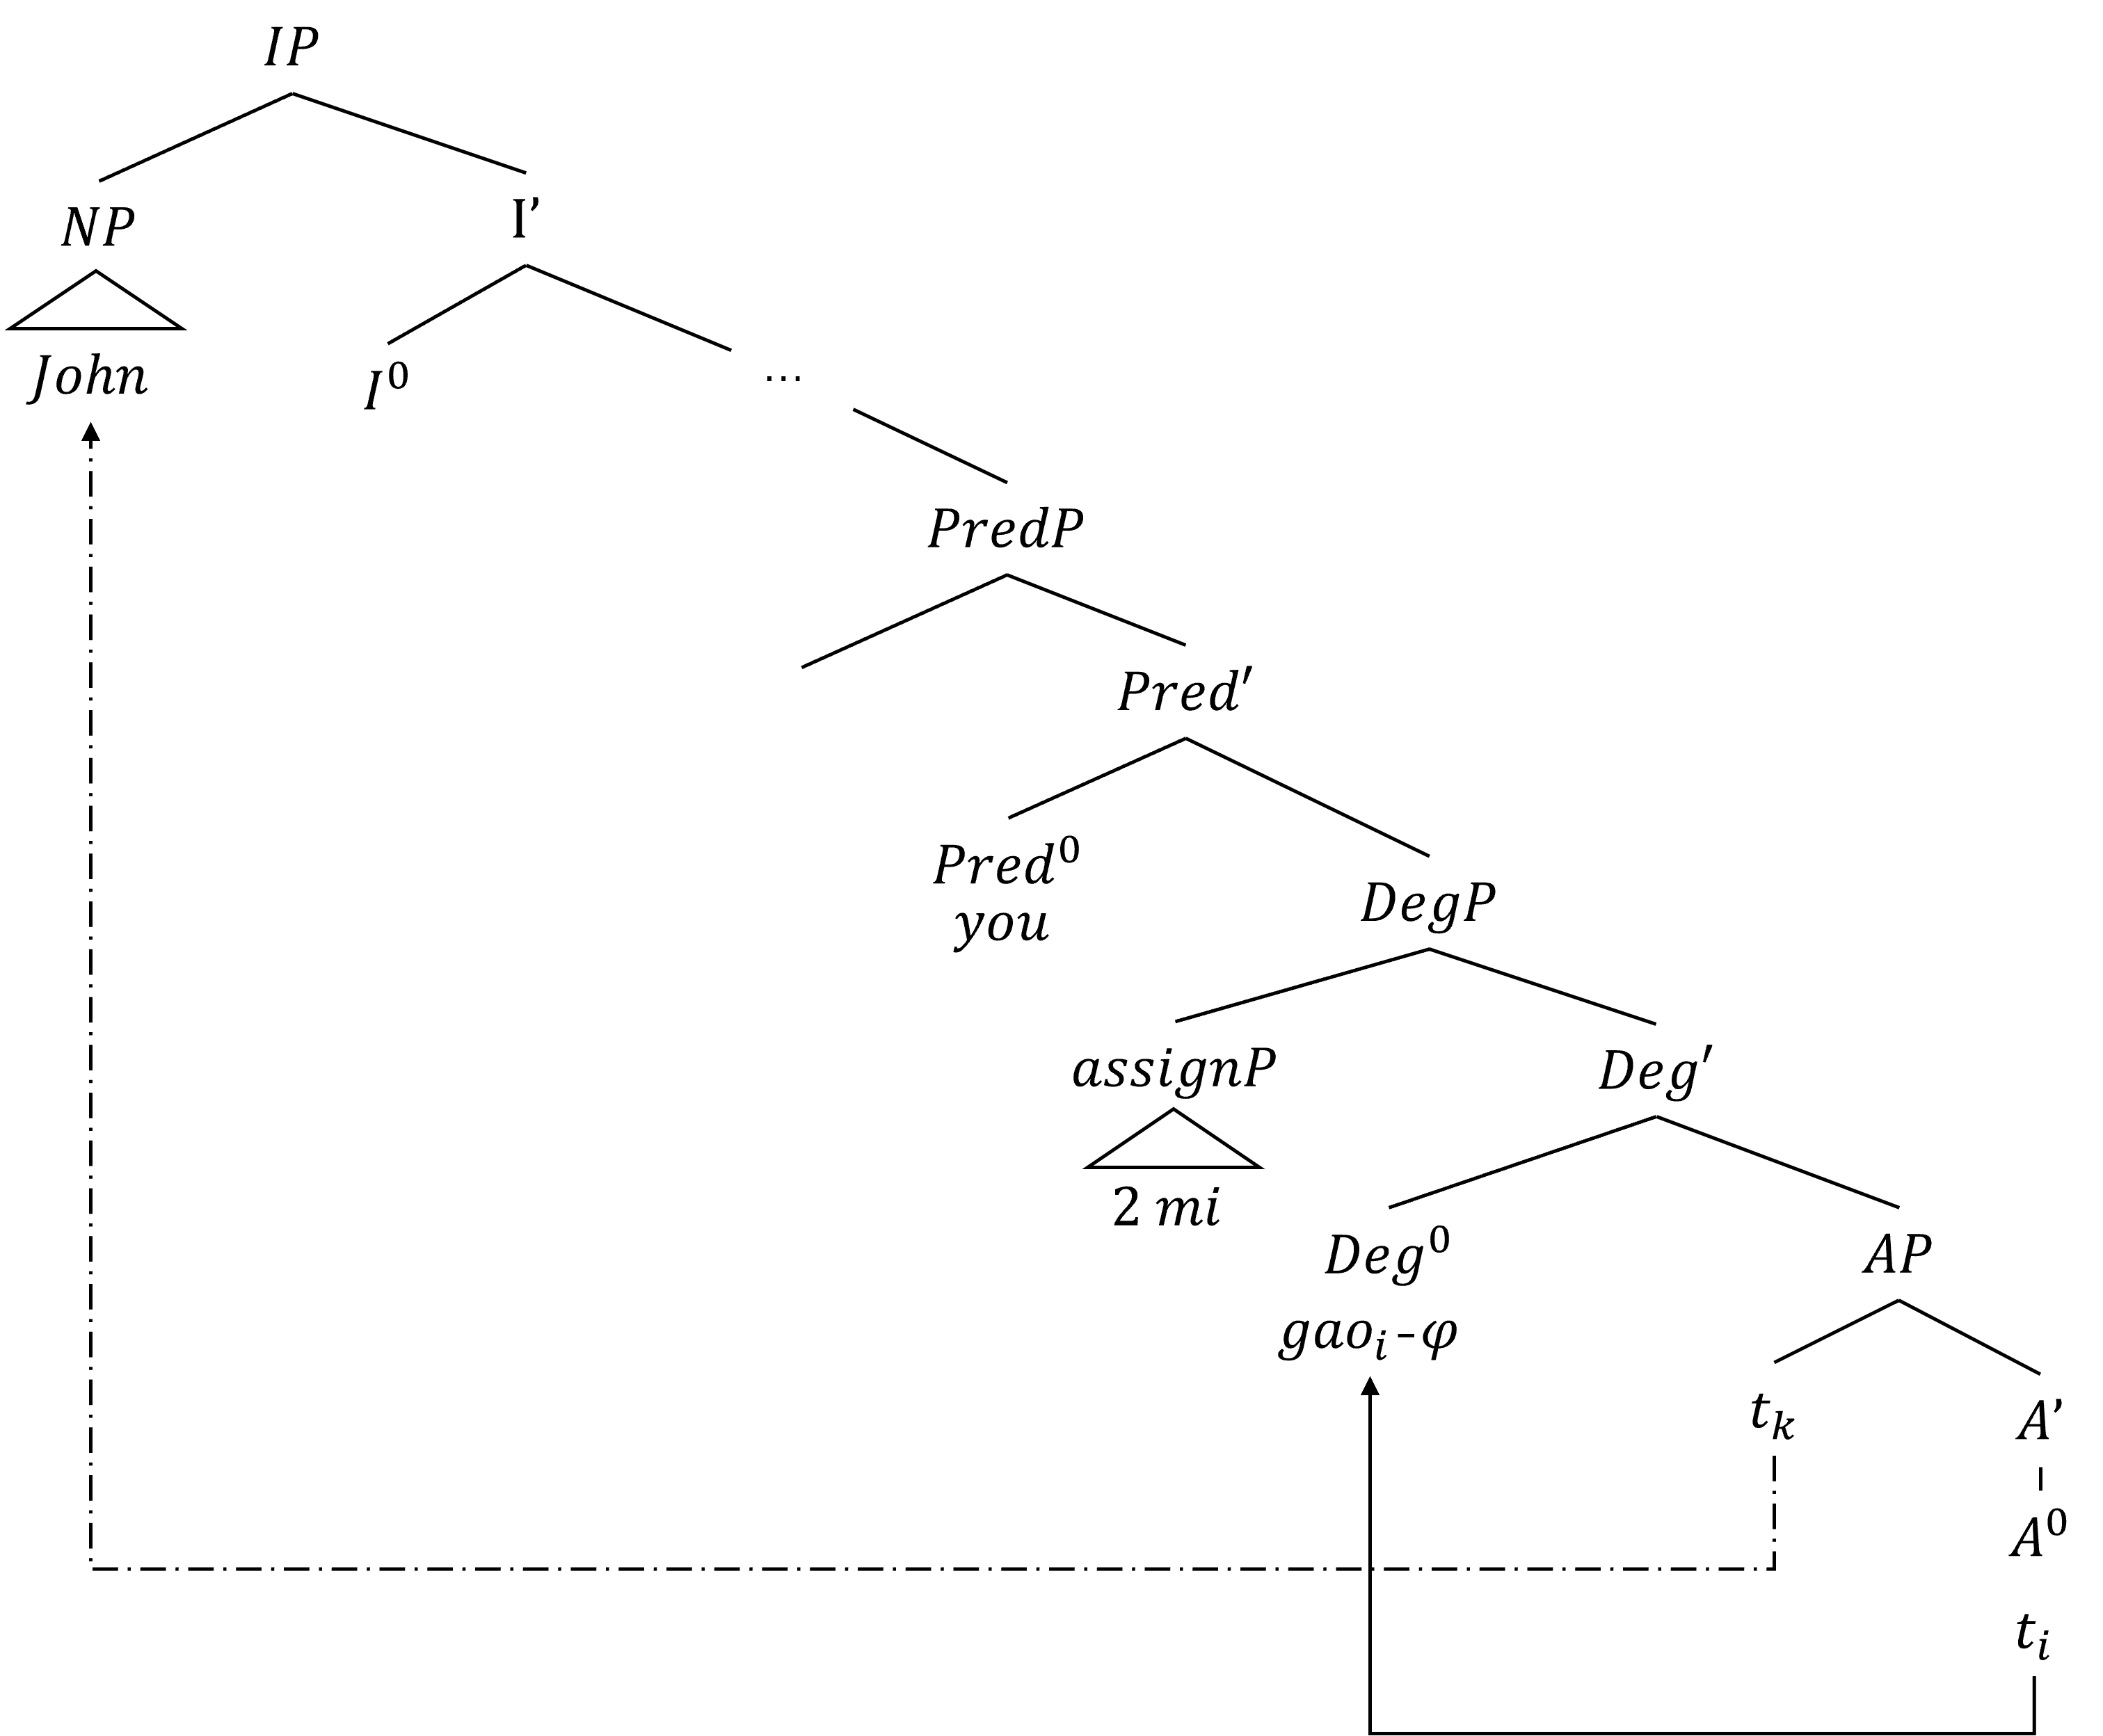
\includegraphics[width=0.7\textwidth]{Pic/assignment_meaning.png}
    \begin{caption}
        \\ \vspace{-1.1ex}
        Structure for assignable meaning.
    \end{caption}
\end{figure}

Example \ref{assignable_example_1_b} gives a truth that the value of \textit{John}'s height is more than 2 meters, the morpheme \textit{duo}(`more') plays the role of suffix of \textit{2mi} and changes it's absolute value to a vague value. From this paper's perspective, \textit{duo}(`more') here does not have independent position in syntactic structure.

The assignable meaning can also build transitive form. The transitive form of \ref{assignable_example_1_a} is \ref{assignable_example_1_a_transitive}, and the construction of this form is shown in \ref{assignable_example_1_a_transitive_tree}. When morpheme \textit{you}(`have') disappears, the gradable adjective moves up to occupy the position of the head of PredP.

\begin{enumerate}
    \item \label{assignable_example_1_a_transitive}
    John gao \enspace 2 mi. \\
    John tall 2 meters. \\
    `John is 2 meters tall.'
\end{enumerate}

\begin{enumerate}
    \item \label{assignable_example_1_a_transitive_tree}
\end{enumerate}

\begin{figure}[H]
    \centering
    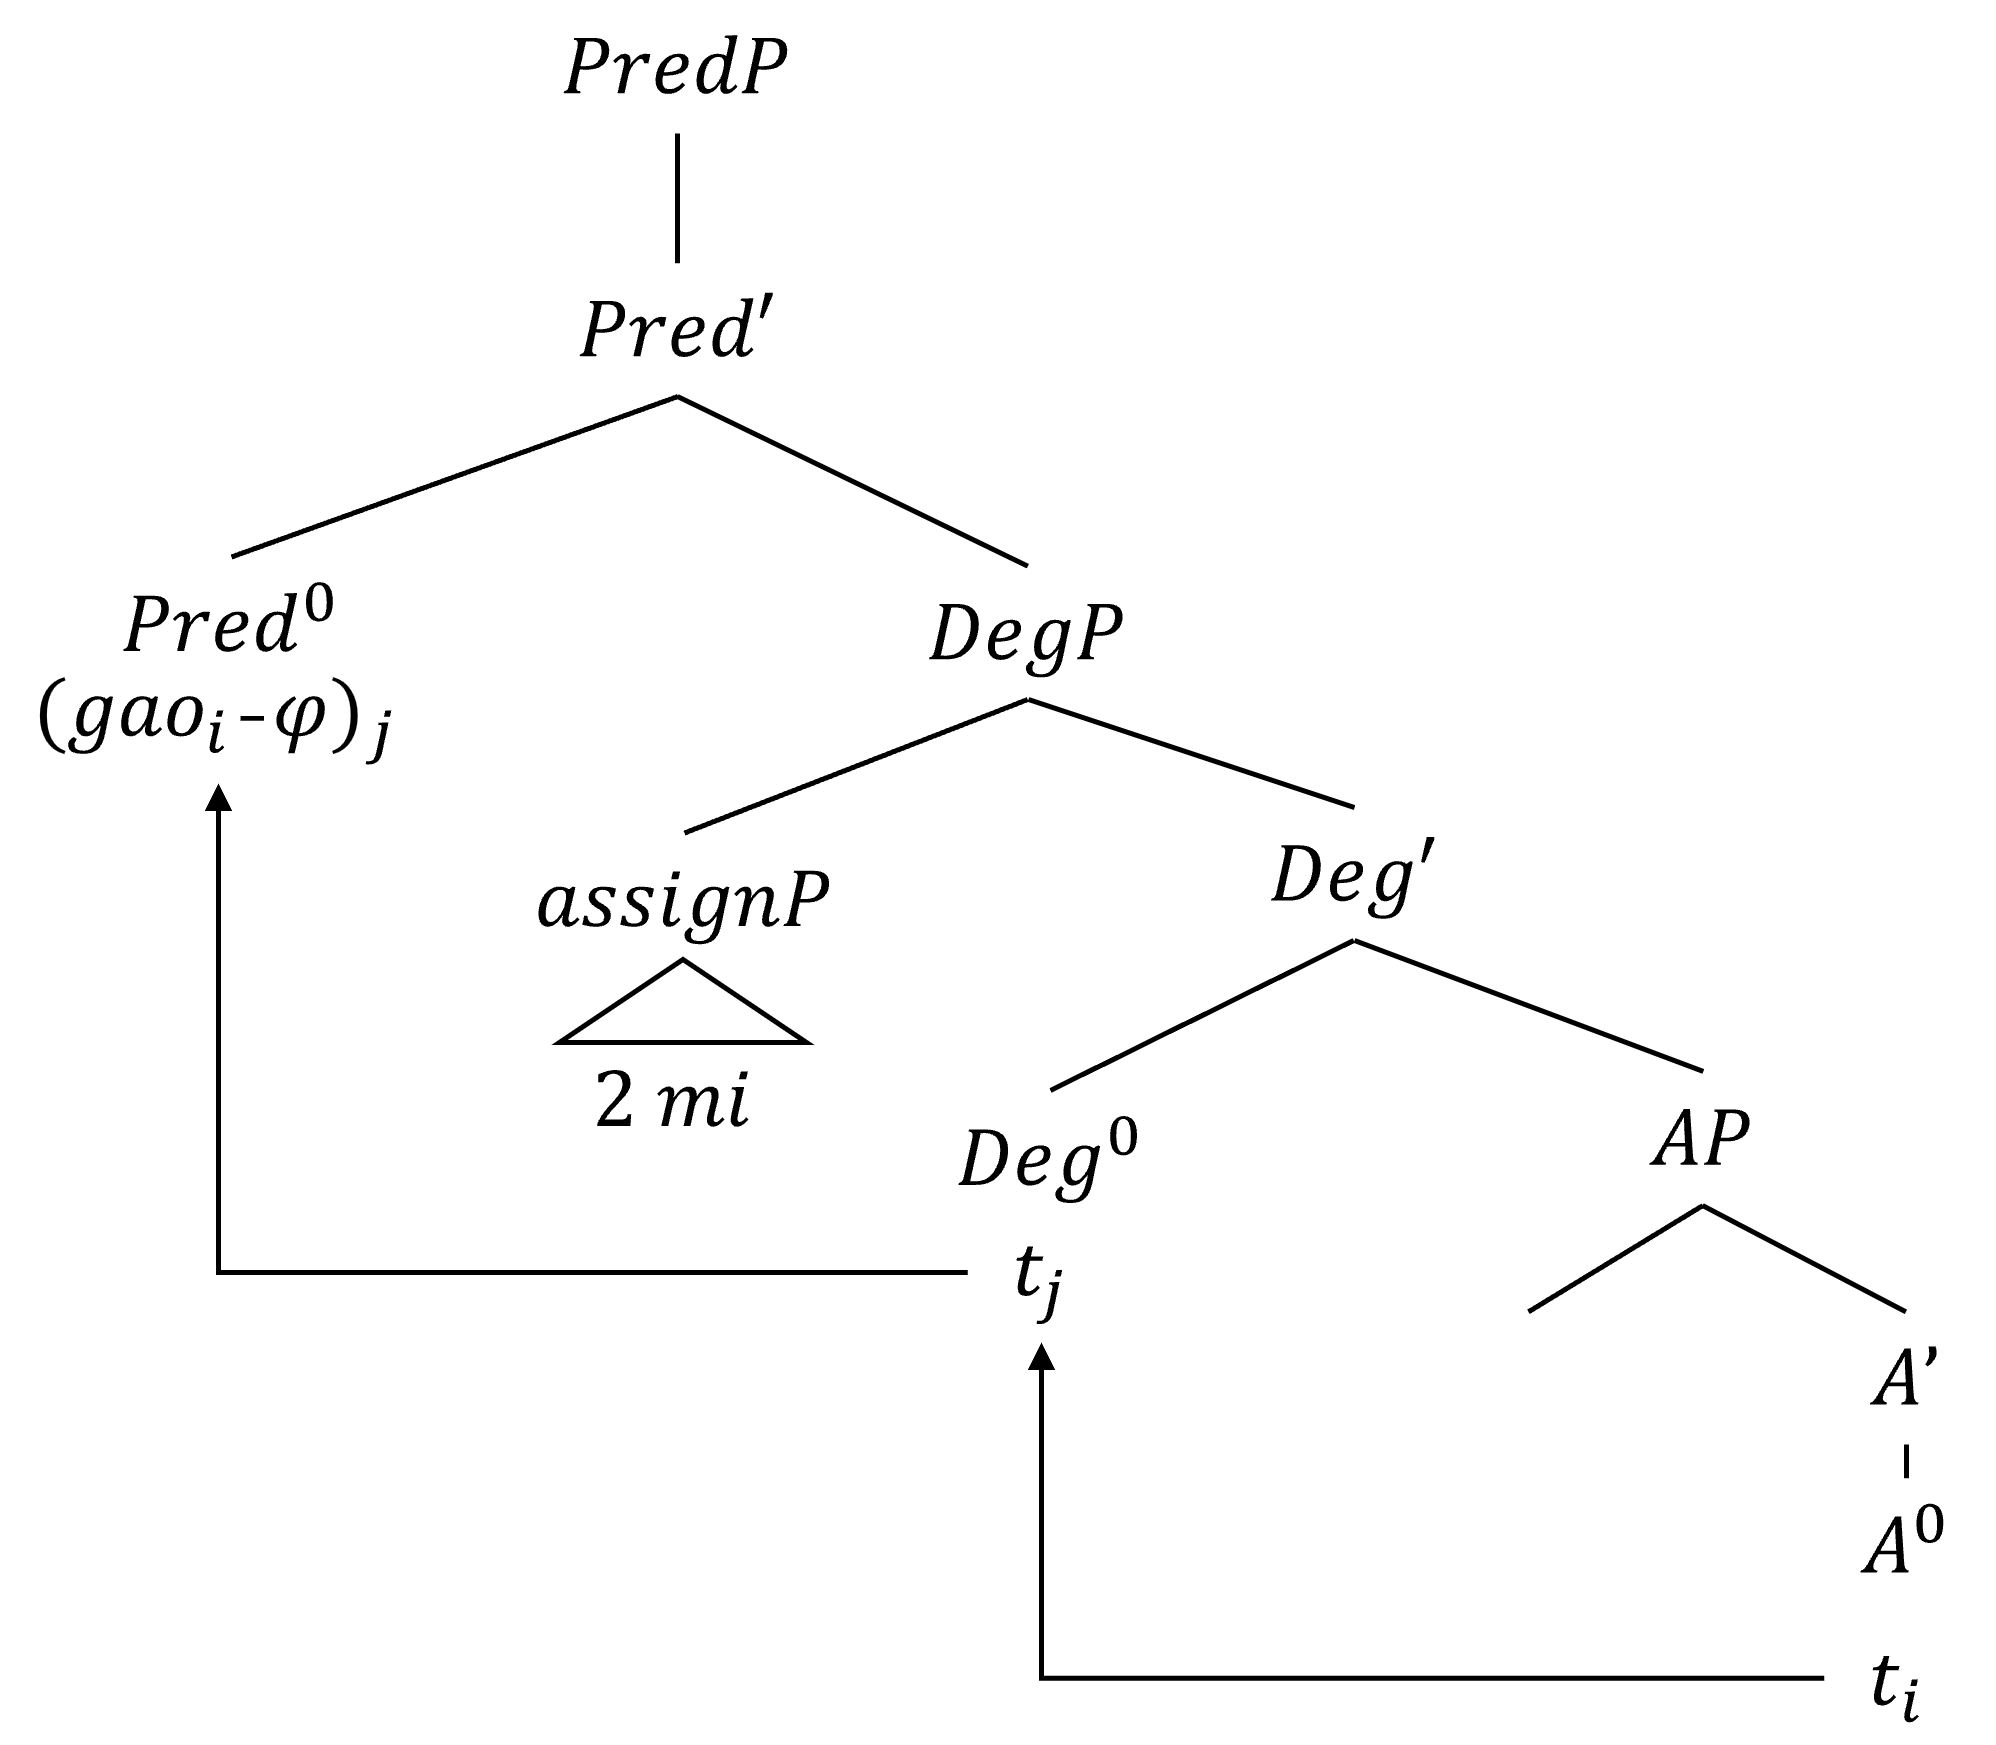
\includegraphics[width=0.5\textwidth]{Pic/assignment_meaning_transitive.png}
    \begin{caption}
        \\ \vspace{-1.1ex}
        Structure for assignable meaning.
    \end{caption}
\end{figure}

Next, the lexical calculation of \ref{assignable_example_1_a} illustrated. The operator $\varphi$ is just a null operator whose job is pass the type $<d,<e,t>>$ to next part. Other deduction is trivial.

\begin{enumerate}
    \item \label{assignable_example_lambda}
    \begin{enumerate}
        \item \label{assignable_example_lambda_a}
        $\begin{aligned}[t]
            [\![\varphi]\!] = \lambda G_{<d,<e,t>>} \lambda d \lambda x.[G(x,d)] \qquad <<d,<e,t>>,<d,<e,t>>>
        \end{aligned}$

        \item \label{assignable_example_lambda_b}
        $\begin{aligned}[t]
            [\![\varphi \enspace gao]\!] 
            &= \lambda G_{<d,<e,t>>} \lambda d \lambda x.[G(x,d)]([\![gao]\!]) \\
            &= \lambda d \lambda x.[height(x) = d] \qquad <d,<e,t>>
        \end{aligned}$

        \item \label{assignable_example_lambda_c}
        $\begin{aligned}[t]
            [\![you \enspace 2m \enspace &\varphi \enspace gao]\!] \\
            &= \lambda d \lambda x.[height(x) = d]([\![you \enspace 2mi]\!]) \\
            &= \lambda d \lambda x.[height(x) = d](2mi) \\
            &= \lambda x.[height(x) = 2mi] \qquad <e,t>
        \end{aligned}$

        \item \label{assignable_example_lambda_d}
        $\begin{aligned}[t]
            [\![John \enspace you \enspace &2m \enspace \varphi \enspace gao]\!] \\
            &= \lambda x.[height(x) = 2mi]([\![John]\!]) \\
            &= height(John)=2m
        \end{aligned}$
        
    \end{enumerate}
\end{enumerate}

\section{COMPARATIVE MEANING}

\subsection{Positivity}

\noindent
Firstly, an example of comparative of positivity is shown in \ref{positivity_example_1}. In literature, it is classified into the positive form. In this paper, we identify this sentence as positivity expressing the comparative meaning, which is significantly different from previous analyses. The reason behind this classification is that the positive judgment of this sentence is based on a comparison between the height of \textit{John} and a value of height considered as the standard by people in mind, which does not need to be indicated or inferred from the context. In fact, this standard value is encoded into the comparative morpheme in positivity sentences. It also deserves some notice that positivity is different from comparatives of superiority with the implicit standard, in that the implicit standard can be inferred from the context rather than encoded by the comparative morpheme itself. The contrast between the sentences in \ref{positivity_example_2_a} and \ref{positivity_example_2_b} can well reveal this point, where the implicit standard is represented as ``Pro'', which can be replaced with the corresponding expression from the context. The meaning of \ref{positivity_example_2_a} and \ref{positivity_example_2_b} is exactly the same, which can also demonstrate the correctness of identifying the implicit standard as ``Pro''. In contrast, we cannot reconstruct the standard from the context for comparative of positivity which explains for the illegitimacy of the sentence in \ref{positivity_example_3_a}.

\begin{enumerate}
    \item \label{positivity_example_1}
    John hen gao.  \\
    John very tall. \\
    `John is very tall'.
\end{enumerate}

\begin{enumerate}
    \item \label{positivity_example_2}
    \begin{enumerate}
        \item \label{positivity_example_2_a}
        John \enspace he Mary shui gao? \\
        John and Mary who tall? \\
        `Who is taller between John and Mary?' \\
        - John Pro gao.\\
        - John Pro tall. \\
        - `John is taller'.

        \item \label{positivity_example_2_b}
        John \enspace he Mary shui gao? \\
        John and Mary who tall? \\
        `Who is taller between John and Mary?' \\
        - John bi Mary gao.\\
        - John than Mary tall. \\
        - `John is taller than Mary'.

        \item \label{positivity_example_3_a}
        * John hen Pro gao.  \\
        \hspace*{0.5em} John very Pro tall. \\
        \hspace*{0.5em} `John is very Pro tall.'

    \end{enumerate}
\end{enumerate}

According to the assumption about two-layer-structure or three-layer-structure on the beginning of this section, given no appearance of DiffP in comparative of positivity, one layer of DegP above AP is considered as the correct syntactic structure for comparative of positivity, which is illustrated as below.

\begin{enumerate}
    \item $John [_{DegP} hen [_{Deg'} gao_i \mbox{-} \xi [_{AP} [_{A'}t_i]]]]$
\end{enumerate}

\begin{figure}[H]
    \centering
    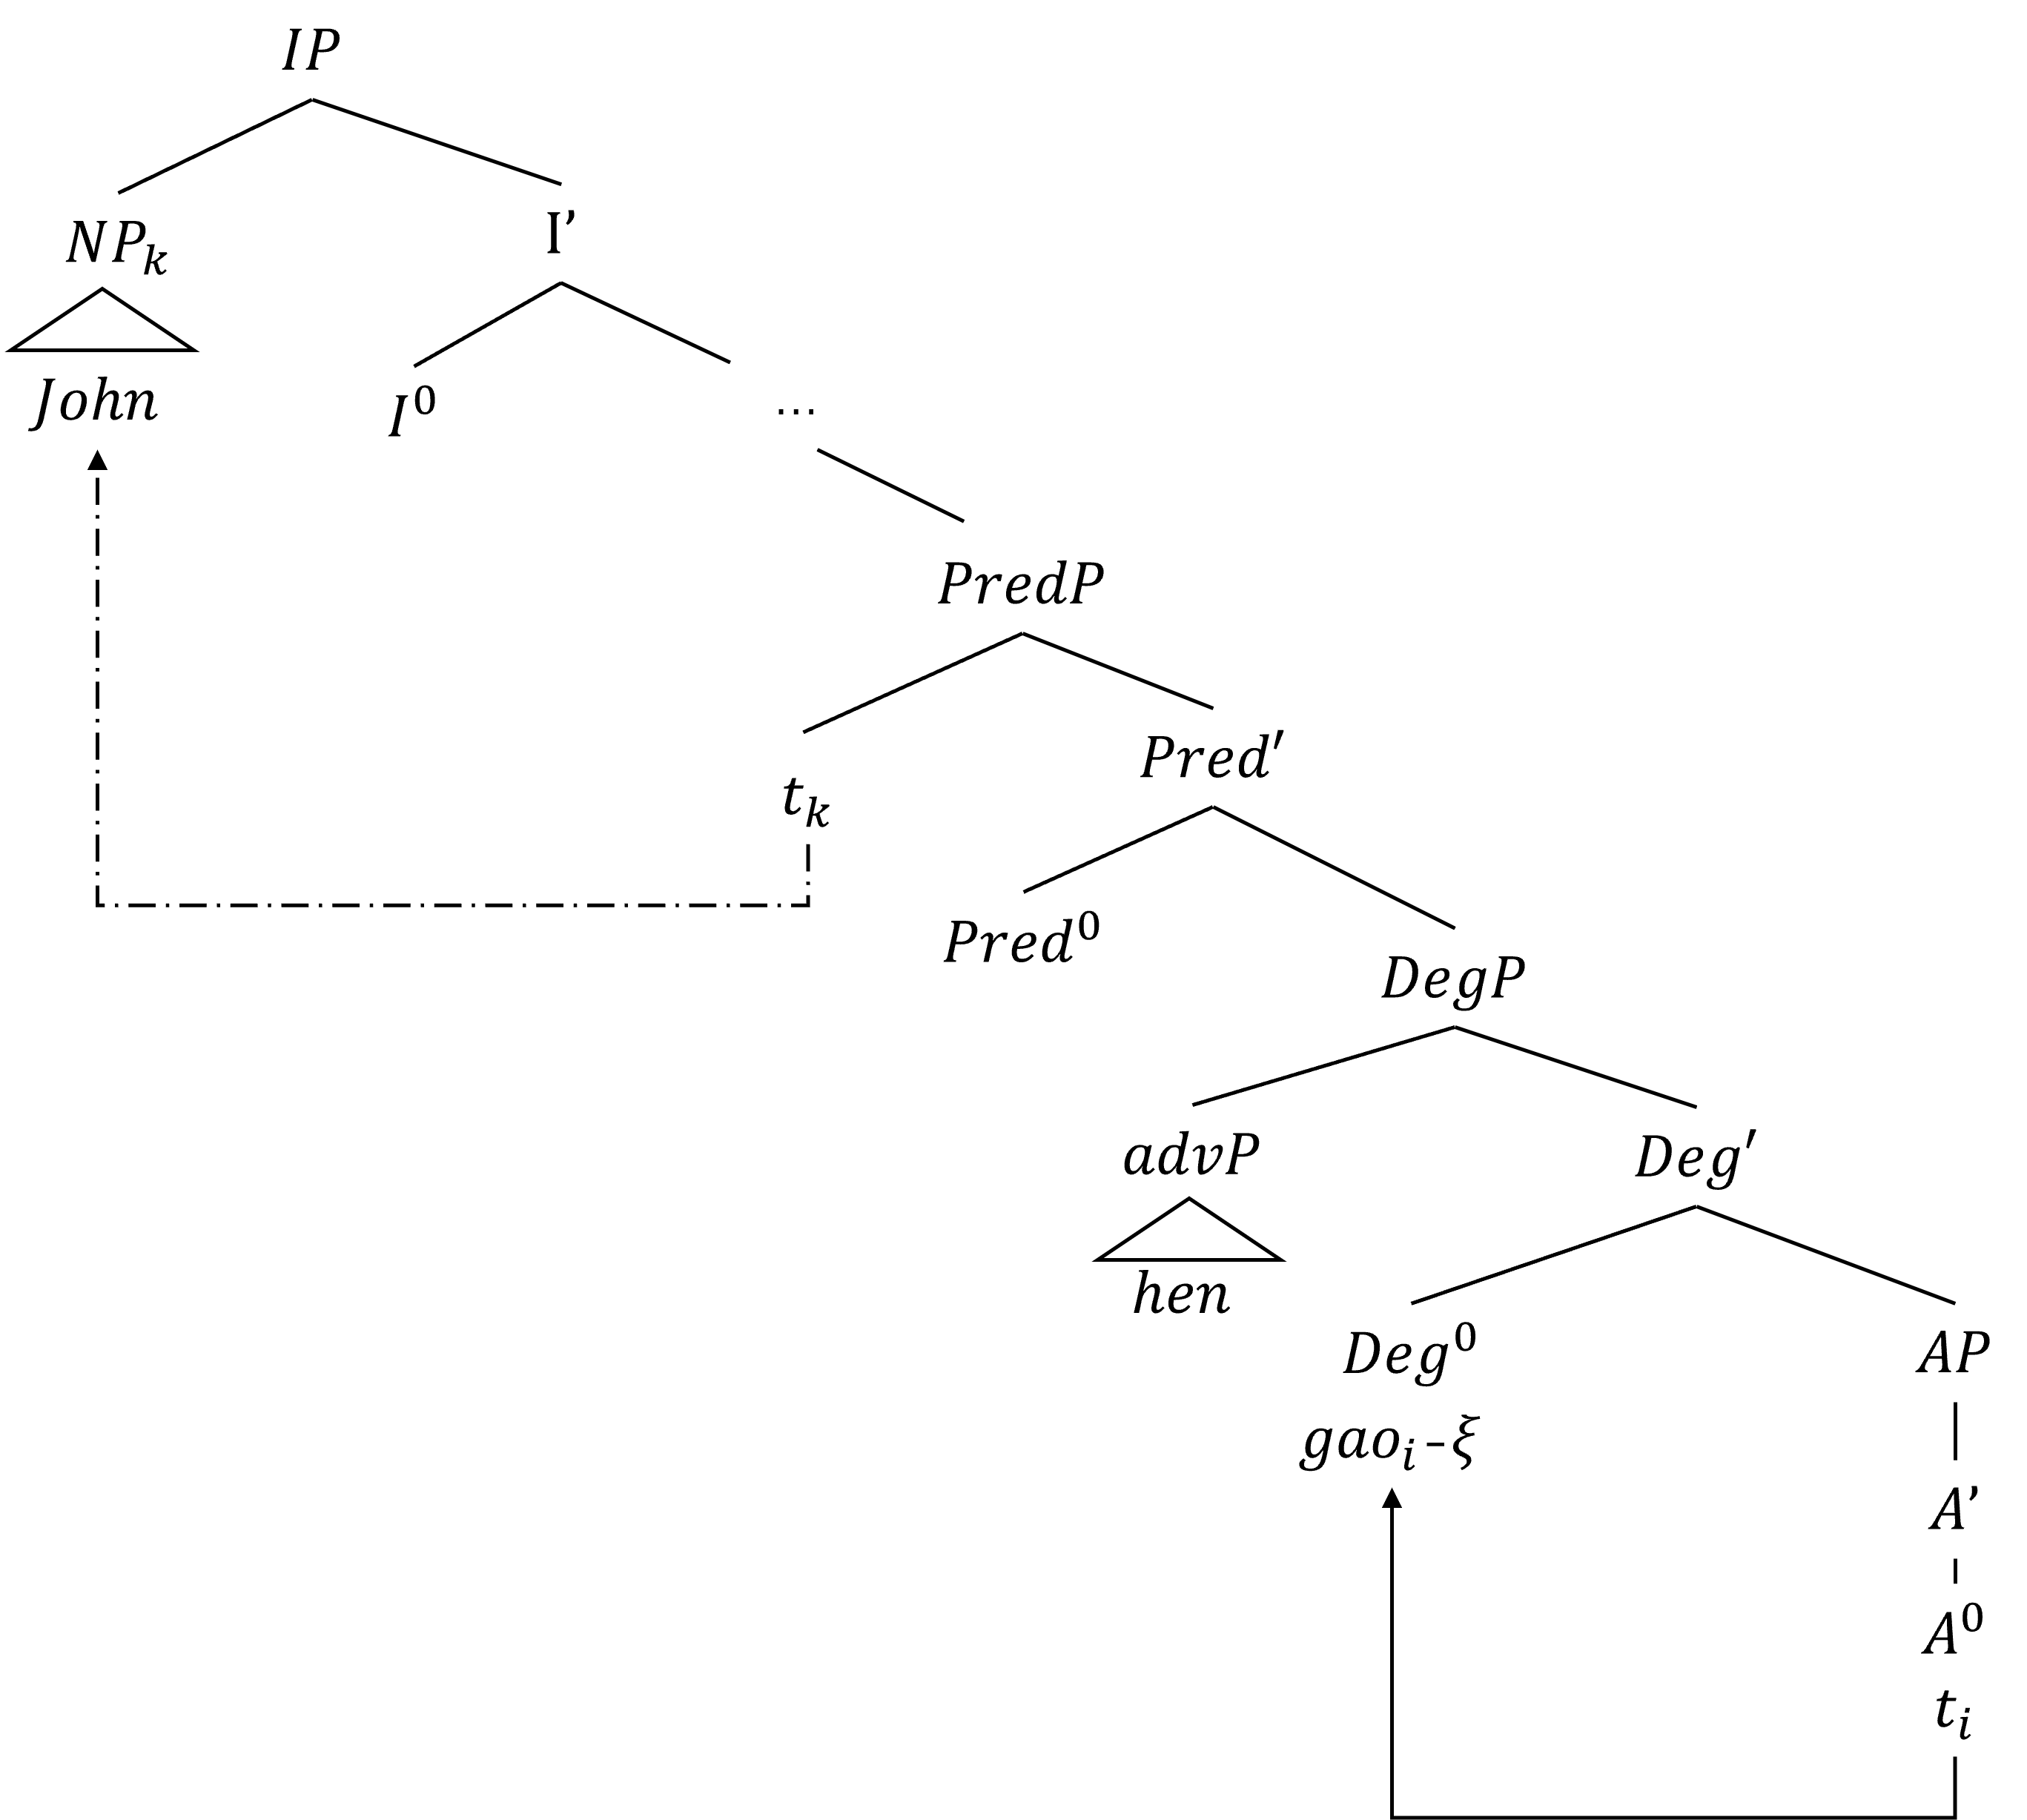
\includegraphics[width=0.5\textwidth]{Pic/positive_structure.png}
    \begin{caption}
        \\ \vspace{-1.1ex}
        Structure for comparative of positivity.
    \end{caption}
\end{figure}

The null nature of DegP head should be licensed by the corresponding expression, which is undertaken by the obligatory \textit{hen}(`very') in this sentence, hence occupies the specifier position of DegP. The obligatoriness of \textit{hen}-like degree adverbs (\textit{feichang}(`much'), \textit{ting}(`very'), etc.) can be reflected by the ungrammaticality of the sentence in \ref{positivity_example_5}.

\begin{enumerate}
    \item \label{positivity_example_5}
    * John gao.  \\
    \hspace*{0.5em} John tall. \\
    \hspace*{0.5em} John is tall'.
\end{enumerate}

However, what should be pointed out is that \textit{hen}(`very') is not prohibited from dropping in other sentences involving positivity. As shown by \ref{positivity_example_6}, \textit{hen}-like degree adverbs are allowed to drop.

\begin{enumerate}
    \item \label{positivity_example_6}
    \begin{enumerate}
        \item \label{positivity_example_6_a}
        John bu gao. \\
        John not tall. \\
        `John is not tall' 

        \item \label{positivity_example_6_b}
        John gao ma? \\
        John tall? \\
        `Is John tall?' 

        \item \label{positivity_example_6_c}
        John gao, Mary ai. \\
        John tall, Mary short. \\
        `John is tall, Mary is short.' 

    \end{enumerate}
\end{enumerate}

This paper will not go into the reasons why sentences like above allow the dropping of \textit{hen}(`very') deeply because they are not canonical clauses, which go beyond the scope of this research. In brief, the sentences above involve other elements related to degree, for example, negative adverb, sentence final particles, focus constructions, etc., which can also function as the licensor of the null degree head \cite{hu2005}.

Now let us turn to the semantics of comparatives of positivity. Klein \cite{klein1980semantics} represents the lexical entry of the degree head in positivity as \ref{positivity_example_7_a}, where $d_{stnd}$ refers to the degree of the corresponding dimension denoted by gradable adjectives which is considered as the standard by people in mind. With the standard degree encoded, the degree head $\xi$ of comparatives of positivity has both evaluative function and type-shift function \cite{rett2014semantics}. Given the equivalence relation which is proven in \ref{positivity_example_7_b}, this paper simplifies the lexical entry of the degree head as \ref{positivity_example_8_a}.

\begin{enumerate}
    \item \label{positivity_example_7}
    \begin{enumerate}
        \item \label{positivity_example_7_a}
        $[\![\xi]\!]=\lambda G_{<d,<e,t>>} \lambda x. \exists d [G(x,d) \land (d=d_{stnd})] \qquad <d,<e,t>,<e,t>>$

        \item \label{positivity_example_7_b}
        $\exists d [G(x,d) \land (d=d_{stnd})] \Leftrightarrow G(x,d_{stnd}) \enspace where \enspace G(x,d) = G \mbox{-} degree(x) \geq d$

        \item \label{positivity_example_8_a}
        $[\![\xi]\!]=\lambda G_{<d,<e,t>>} \lambda x. [G(x,d_{stnd})] \qquad <d,<e,t>,<e,t>>$

    \end{enumerate}
\end{enumerate}

With the lexical entry of the gradable adjective \textit{tall} given in \ref{tallLE_re_a}, the meaning of the sentence in \ref{positivity_example_8_a_fuck} can be figured out successfully following the semantic calculations illustrated in \ref{positivity_example_8}, which is paraphrased as \ref{positivity_example_8_d}.

\begin{enumerate}
    \item \label{positivity_example_8}
    \begin{enumerate}

        \item \label{positivity_example_8_a_fuck}
        John hen gao. \\
        John very tall. \\
        `John is very tall.'

        \item \label{positivity_example_8_b}
        $\begin{aligned}[t]
            [\![\xi \enspace gao]\!] &= \lambda G_{<d,<e,t>>} \lambda x. [G(x,d_{stnd})]([\![gao]\!]) \\
            &= \lambda x.[height(x) \geq d_{stnd}] \qquad <e,t>
        \end{aligned}$

        \item \label{positivity_example_8_c}
        $\begin{aligned}[t]
            [\![John \enspace \xi \enspace gao]\!] &= \lambda x.[height(x) \geq d_{stnd}]([\![John]\!]) \\
            &= height(John) \geq d_{stnd}
        \end{aligned}$

        \item \label{positivity_example_8_d}
        \ref{positivity_example_8_c} is paraphrased as ``the height of John exceeds the standard degree considered as tall by people in mind''

    \end{enumerate}
\end{enumerate}

\subsection{Superiority}

\noindent
Most of previous studies are inclined to appoint too heavy semantic function to one of the degree head and as a result make the semantic function of the other degree head marginal and transparent. What is worse, the ``greater than'' meaning encoded in the lexical entry of gradable adjective is seized by a degree head which should not have been in charge of indicating the ordering relation between the comparee and the standard. In addition, the transfer of the ``greater than'' meaning from gradable adjectives to the degree head would give rise to incorrect reading of sentences made out of gradable adjectives with DiffP.

Here we illustrate this fatal disadvantage with an instance from von Stechow \cite{von1984a}. In his analysis, the comparative morpheme \textit{er}(`than') in English undertakes the ``greater than'' meaning, as well as serves to usher in the gap between the comparee and the standard along the dimension of scale denoted by the gradable adjective in the case of comparative constructions with differential phrase. In \ref{maomao_2_12} is displayed its lexical entry. The comparative morpheme successively absorb three arguments, i.e., the property of degree argument $D$ determined by the standard, the degree argument $d$ denoted by the differential phrase and  the property of degree argument $G$ determined by the comparee.

\begin{enumerate}
    \item \label{maomao_2_12}
    $[\![er]\!] = \lambda D_{<d,t>} \lambda d' \lambda G_{<d,t>} . [Max(G) \geq Max(D) + d'] \qquad <<d,t>,<d,<<d,t>,t>>>$
\end{enumerate}

Example in \ref{maomao_2_13_a} for instance and apply von Stechow's analysis to this sentence. \ref{maomao_2_13_b} roughly shows the logical form. Although von Stechow's analysis is built on sentences in English, the core spirit can be well transplanted to analysis of Mandarin comparative constructions.

Given that there is no overt comparative morpheme in \ref{maomao_2_13_a}, \textit{comp} is used to indicate the covert comparative morpheme (i.e., equivalent to mu in our notation system). Due to the same meaning and function with \textit{er}(`than') in English, its lexical entry shown as \ref{maomao_2_13_c} is also as same as the lexical entry of \textit{er}(`than') given in \ref{maomao_2_12}. The comparison between two individuals, i.e., the comparee and the standard, is shifted to the comparison between properties of degree, of which the formalizations are respectively displayed in (13d) and (13e). The technical details involved are not discussed here given that they are not related to the core interpretation of the comparative morpheme which is the current essential issue. Based on semantic compositionality, after the comparatives morpheme successively absorbing the property of degree determined by the standard \textit{Mary}, the degree denoted by the differential phrase \textit{2 limi}(`2 centimeters'), and the the property of degree determined by the comparee \textit{John}, the ultimate formalization is derived out as \ref{maomao_2_13_f}, which is paraphrased as ``the maximal degree to which John is tall exceeds or equal to the maximal degree to which Mary is tall plus 2 limi''. Its equivalent form is given in \ref{maomao_2_13_g}, but in a more concise way. The formalization implies ``John can be more than 2 limi taller than Mary'', which does not adhere to our understanding of the sentence given in \ref{maomao_2_13_a} that ``John is exactly 2 centimeters taller than Mary''. As a result, von Stechow's analysis of the comparative morpheme fails to derive the correct semantic interpretation for comparatives of Superiority with DiffP. This failure is owed to the lack of clear division of labour among different functional morphemes and the gradable adjective.

\begin{enumerate}
    \item \label{maomao_2_13}
    \begin{enumerate}
        \item \label{maomao_2_13_a}
        John \enspace bi \enspace Mary \enspace gao \enspace \enspace 2 limi. \\
        John than Mary \enspace tall 2 centimeters. \\
        `John is 2 centimeters taller than Mary.'

        \item \label{maomao_2_13_b}
        $[_{DegP}[_{DegP'}[_{PP}bi \enspace op_i \enspace Mary \enspace d_i \enspace gao] comp][_{DiffP}2limi]]_j John \enspace d_j gao$

        \item \label{maomao_2_13_c}
        $\begin{aligned}[t]
            [\![comp]\!]&=\lambda D_{<d,t>} \lambda d' \lambda G_{<d,t>} . [Max(G) \geq Max(D) + d'] \\ & <<d,t>,<d,<<d,t>,t>>>
        \end{aligned}$

        \item \label{maomao_2_13_d}
        $[\![bi \enspace op_i \enspace Mary \enspace d_i \enspace gao]\!]
        = \lambda d.[height(Mary) \geq d] \qquad <d,t>$

        \item \label{maomao_2_13_e}
        $[\![John \enspace gao]\!] = \lambda d.[height(John) \geq d] \qquad <d,t>$

        \item \label{maomao_2_13_f}
        $\begin{aligned}[t]
            [\![John &\enspace bi \enspace Mary \enspace gao \enspace 2 limi]\!] 
            = Max(\lambda d.[height(John) \geq d]) \\ &\geq Max(height(Mary) \geq d) + 2limi
        \end{aligned}$

        \item \label{maomao_2_13_g}
        \ref{maomao_2_13_f} $\Leftrightarrow height(John) \geq height(Mary) + 2limi$

    \end{enumerate}
\end{enumerate}

This clear division of labor in terms of the semantic meaning bore by each component is crucial for the whole analysis and this perspective is also significantly different from previous analyses.

\subsubsection{Superiority without differential phrase}

\noindent
In \ref{superiority_example_1}, there are serval examples which are comparatives of superiority without differential phrase. And the standard of three examples are different, \ref{superiority_example_1_a} has a specific value (or saying standard value) to compare, \ref{superiority_example_1_b} compares with a single individual, \ref{superiority_example_1_c} treats a set of individuals as compare target. These three examples represent three classification of standards in comparatives, which has been discussed in the introduction. And next, we will give analyses about these examples from the syntactic perspective and the semantic perspective respectively.

\begin{enumerate}
    \item \label{superiority_example_1}
    \begin{enumerate}
        \item \label{superiority_example_1_a}
        John \enspace bi \enspace \enspace \enspace 1.7 mi \enspace \enspace \enspace gao. \\
        John than \enspace 1.7 meters tall. \\
        `John is taller than 1.7 mi.' 

        \item \label{superiority_example_1_b}
        John \enspace bi \enspace Mary gao. \\
        John than Mary tall. \\
        `John is taller than Mary.' 

        \item \label{superiority_example_1_c}
        John zai \enspace yiban \enspace \enspace zui \enspace gao. \\
        John in \enspace class.one most tall. \\
        `John is tallest in class one' 

    \end{enumerate}
\end{enumerate}

According to the assumption in the beginning of this section, Superiority sentences without DiffP are assumed to project only one functional layer above AP, taking ``DegP-AP'' as their syntactic structure. No matter what type of the standard is taken, the general structure is almost the same, and the standard's position in structure is called StndP. For achieving a unifying analysis, we use $\xi_n$ to represent for the degree head in higher DegP, in which the index $n$ is to distinguish variants of the degree head. The syntactic structure of comparative of superiority without DiffP is illustrated in \ref{superiority_structure}, with clear account of the index of $\xi_n$ given in \ref{superiority_example_2}. Their lexical entries and lexical calculations will be displayed soon.

\begin{enumerate}
    \item \label{superiority_structure}
    $\begin{aligned}[t]
        [_{IP} &[CompareeP_k] [_{I^{\prime}} I^{0} [_{...}[_{PredP} t_k [_{Pred'} bi/zai [[_{DegP} [StndP] [_{Deg^{\prime}} A_i^0\mbox{-}\xi_{n} [_{AP} [_{A^{\prime}} t_i]]]]]]]]]] \\ 
        &n \in \{1, 2, 3\}
    \end{aligned}$
\end{enumerate}

\begin{figure}[H]
    \centering
    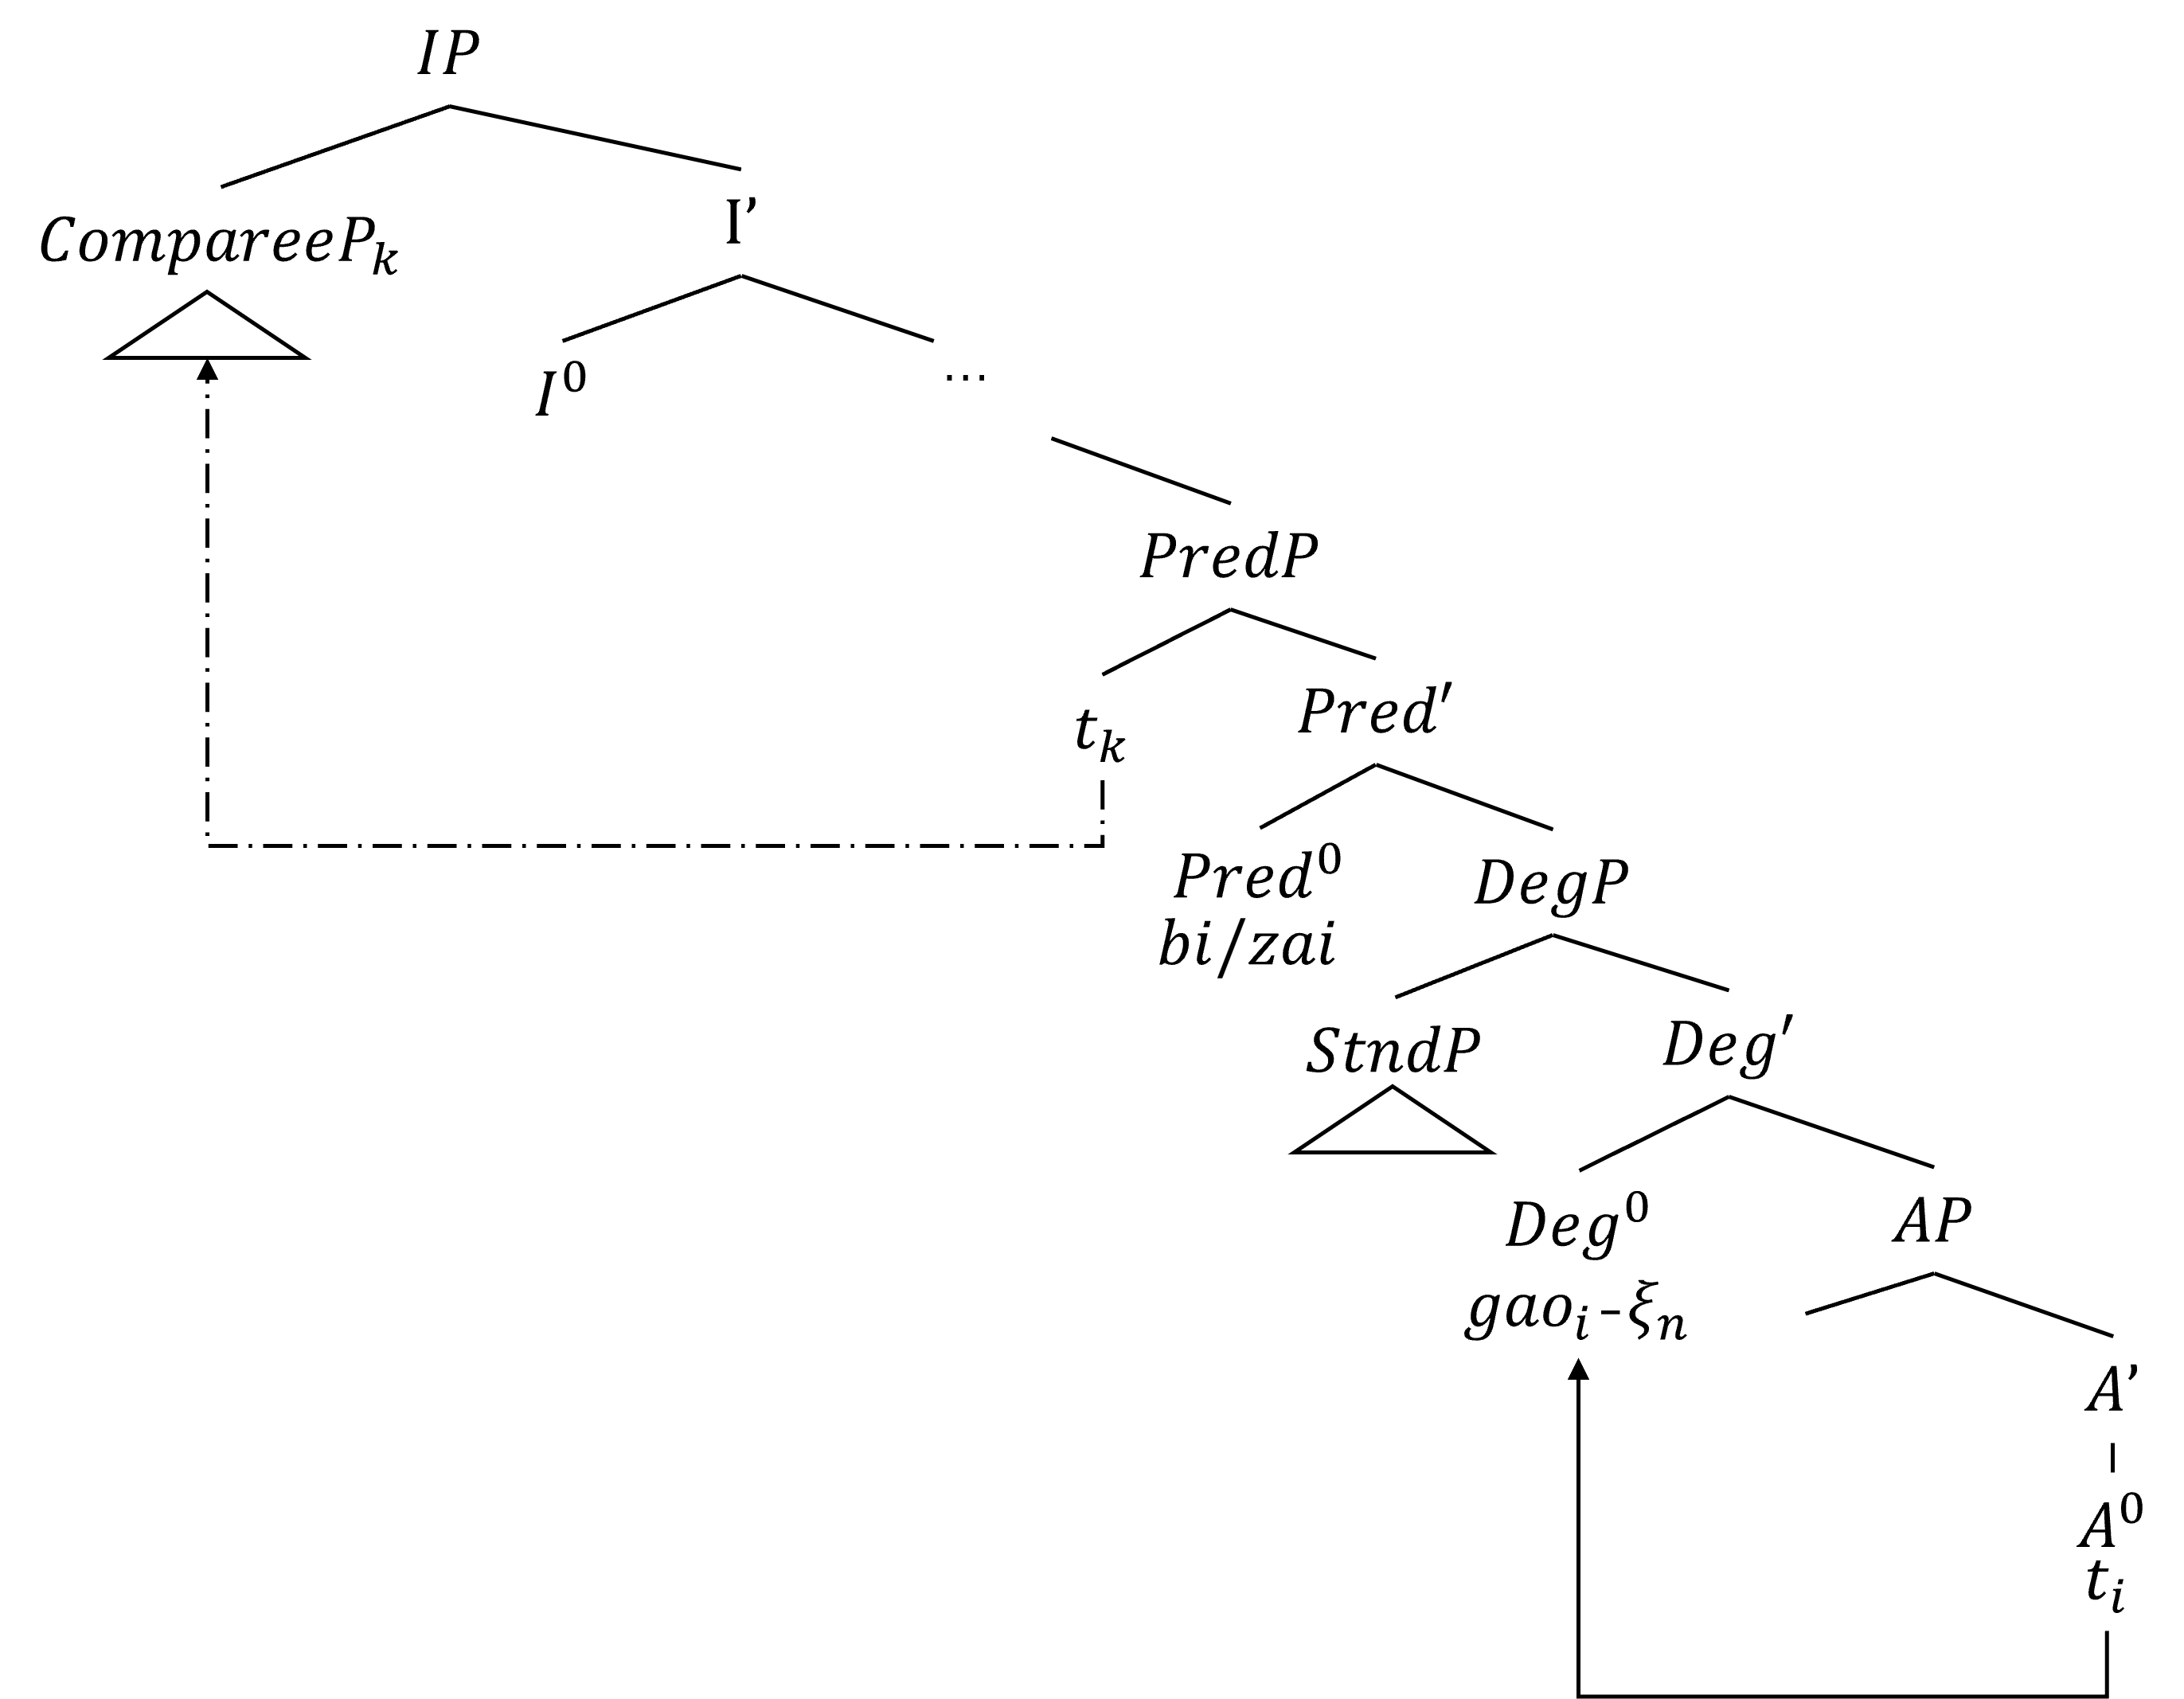
\includegraphics[width=0.6\textwidth]{Pic/superiority_structure.png}
    \begin{caption}
        \\ \vspace{-1.1ex}
        Structure for comparative of superiority without DiffP.
    \end{caption}
\end{figure}

\begin{enumerate}
    \item \label{superiority_example_2}
    \begin{enumerate}
        \item \label{superiority_example_2_a}
        for $\xi_n$, $n=1$ if and only if the standard is a degree;

        \item \label{superiority_example_2_b}
        for $\xi_n$, $n=2$ if and only if the standard is an individual;

        \item \label{superiority_example_2_c}
        for $\xi_n$, $n=3$ if and only if the standard is a set of individuals;

    \end{enumerate}
\end{enumerate}

Another position worth to be noticed is the predicate phrase (PredP), whose head is occupied by the morpheme \textit{bi}(`than') in \ref{superiority_example_1}. In traditional analysis, most researchers believe the morpheme \textit{bi}(`than') should belong to a phrase called biP which lands at the specifier of DegP. But this paper argues that the \textit{bi}(`than') is the predicator in the sentence, which is kind of different with English. The core reason is to build the transitive comparative, where the differential phrase is obligatory. However, why DiffP is obligatory for transitive comparative is still a mystery. 

Some more words perhaps should be said about instantiation of the degree head. When the standard is a degree or an individual, the degree morpheme could be a null morpheme $\emptyset$, could have phonetic realization as \textit{geng}(`more'), \textit{hai}(`still'), etc, as shown in \ref{superiority_example_3_a}. It should be pointed out the null functional morpheme  always only has the neutral meaning, while its co-existent counterpart with phonetic realizations should have some minor distinct meaning, otherwise it is redundant to use  different morphemes to undertake the single one function as well as express exactly the same meaning. When comes to the standard as a set of individuals, the degree morpheme should be consistently realized as \textit{zui}(`most'), which hosts the neutral meaning, as shown by \ref{superiority_example_4_a}.

\begin{enumerate}
    \item \label{superiority_example_3}
    \begin{enumerate}
        \item \label{superiority_example_3_a}
        John \enspace bi \enspace Mary (geng/hai) gao. \\
        John than Mary \enspace \enspace much \enspace \enspace tall. \\
        `John is much taller than Mary.'

        \item \label{superiority_example_4_a}
        John zai \enspace yiban *(zui) \enspace gao. \\
        John in class.one *(most) tall. \\
        `John is tallest in class one.'


    \end{enumerate}
\end{enumerate}

When the degree head is a bound morpheme with phonetic realization like \textit{geng}(more) and \textit{zui}(most) or a null morpheme $\emptyset$ which is also a bound morpheme, the gradable adjective moves up to combine with the degree head because bound morphemes cannot stand alone \cite{hebook}. The comparee denoted by NP(DP) is base generated in the specifier of PredP, where no Case can be assigned. Therefore the comparee moves to the specifier of the IP to be assigned Nominative Case. 

Then for the semantic part. According to Abney's DegP hypothesis, the functional projection DegP in comparative of superiority sentences consistently serves to bind the extra argument $d$ in the lexical entry of gradable adjectives by introducing the standard in comparative meaning. In terms of the function of the head of DegP, we make a significant  difference from previous scholars. The majority of previous analyses \cite{von1984a,bale2008} considers the comparative morpheme which occupies the head position of DegP bear the crucial ``greater than'' meaning in making comparison. However, the lexical entry of gradable adjectives shown in \ref{tallLE_re_a} which is repeated here as \ref{tallLE_re_re}, has already included ``the partial ordering relation'' which is established between the comparee and the standard along the dimension of scale denoted by the gradable adjective, which conveys the ``greater than'' meaning. Hence it is quite redundant to appoint another morpheme to denote the ``greater than'' meaning.  Here we assume that the functional head of DegP severs to usher in the standard as well as adjust the the method of absorbing the standard accordingly so that it can be incorporated into the degree argument of the gradable. As a result, the semantic type and lexical entry of the head of DegP are variable corresponding to distinct standard types.

\begin{enumerate}
    \item \label{tallLE_re_re}
    $[\![tall]\!]=\lambda d \lambda x.[Height(x) \geq d] \qquad <d,<e,t>>$
\end{enumerate}

Semantic formalizations of these three variants $\xi_1$, $\xi_2$ and $\xi_3$ are elaborated as below respectively.

\paragraph{Specific value standard:}

Semantic calculations in \ref{superiority_example_5} corresponds to the sentence in \ref{superiority_example_1_a} (re-written in \ref{superiority_example_1_a_re}) where the standard is a degree typed $d$. The lexical entry of the degree head $\xi_1$ is given in \ref{superiority_example_5_a}. The output proposition is paraphrased as \ref{superiority_example_5_e}, which derives the meaning of the sentence correctly.

\begin{enumerate}
    \item \label{superiority_example_1_a_re}
    John \enspace bi \enspace \enspace 1.7 mi \enspace \enspace \enspace gao. \\
    John than 1.7 meters gao. \\
    `John is taller than 1.7 mi.' 
\end{enumerate}

\begin{enumerate}
    \item \label{superiority_example_5}
    \begin{enumerate}
        \item \label{superiority_example_5_a}
        $[\![\xi_1]\!] = \lambda G_{<d,<e,t>>} \lambda d \lambda x.[G(x,d)] \qquad <<d,<e,t>>,<d,<e,t>>>$

        \item \label{superiority_example_5_b}
        $\begin{aligned}[t]
            [\![\xi_1 \enspace gao]\!] &= \lambda G_{<d,<e,t>>} \lambda d \lambda x.[G(x,d)]([\![gao]\!]) \\
            &= \lambda d \lambda x.[height(x) \geq d] \qquad <d,<e,t>>
        \end{aligned}$

        \item \label{superiority_example_5_c}
        $\begin{aligned}[t]
            [\![1.7mi \enspace \xi_1 \enspace gao]\!]
            &= \lambda d \lambda x.[height(x) \geq d](1.7mi) \\
            &= \lambda x.[height(x) \geq 1.7mi] \qquad <e,t>
        \end{aligned}$

        \item \label{superiority_example_5_c_1}
        $\begin{aligned}[t]
            [\![bi]\!] = \lambda P.[P] \qquad <<e,t>,<e,t>>
        \end{aligned}$

        \item \label{superiority_example_5_c_2}
        $\begin{aligned}[t]
            [\![bi \enspace 1.7mi \enspace \xi_1 \enspace gao]\!] &= [\![bi]\!]([\![1.7mi \enspace \xi_1 \enspace gao]\!])
            &= \lambda x.[height(x) \geq 1.7mi] \qquad <e,t>
        \end{aligned}$

        \item \label{superiority_example_5_d}
        $\begin{aligned}[t]
            [\![John \enspace bi \enspace 1.7mi \enspace \xi_1 \enspace gao]\!] &= \lambda x.[height(x) \geq 1.7mi](John) \\
            &= height(John) \geq 1.7mi
        \end{aligned}$

        \item \label{superiority_example_5_e}
        \ref{superiority_example_5_d} is paraphrased as ``the height of John exceeds 1.7 metres''

    \end{enumerate}
\end{enumerate}

\paragraph{Single individual standard:}

Semantic calculations in \ref{superiority_example_6} corresponds to the sentence in \ref{superiority_example_1_b} (re-written in \ref{superiority_example_1_b_re}) where the standard is an individual typed $e$. The lexical entry of the degree head $\xi_2$ is given in \ref{superiority_example_6_a}. The output proposition is paraphrased as \ref{superiority_example_6_e}.

\begin{enumerate}
    \item \label{superiority_example_1_b_re}
    John \enspace bi \enspace Mary gao. \\
    John than Mary tall. \\
    `John is taller than Mary.'
\end{enumerate}

\begin{enumerate}
    \item \label{superiority_example_6}
    \begin{enumerate}
        \item \label{superiority_example_6_a}
        $[\![\xi_2]\!] = \lambda G_{<d,<e,t>>} \lambda y \lambda x.[G(x,G \mbox{-} degree(y))] \qquad <<d,<e,t>>,<e,<e,t>>>$

        \item \label{superiority_example_6_b}
        $\begin{aligned}[t]
            [\![\xi_2 \enspace gao]\!] 
            &= \lambda G_{<d,<e,t>>} \lambda y \lambda x.[G(x,G\mbox{-}degree(y))]([\![gao]\!]) \\
            &= \lambda y \lambda x.[height(x) \geq height(y)] \qquad <e,<e,t>>
        \end{aligned}$

        \item \label{superiority_example_6_c}
        $\begin{aligned}[t]
            [\![\enspace Mary \enspace & \xi_2 \enspace gao]\!] \\
            &= \lambda y \lambda x.[height(x) \geq height(y)]([\![\enspace Mary]\!]) \\
            &= \lambda y \lambda x.[height(x) \geq height(y)](Mary) \\
            &= \lambda x.[height(x) \geq height(Mary)] \qquad <e,t>
        \end{aligned}$

        \item \label{superiority_example_6_d}
        $\begin{aligned}[t]
            [\![John \enspace bi \enspace & Mary \enspace \xi_2 \enspace gao]\!] \\
            &= \lambda x.[height(x) \geq height(Mary)](John) \\
            &= height(John) \geq height(Mary)
        \end{aligned}$

        \item \label{superiority_example_6_e}
        \ref{superiority_example_6_d} is paraphrased as ``the height of John exceeds the height of Mary''

    \end{enumerate}
\end{enumerate}

\paragraph{Individual set standard:}

Semantic calculations in \ref{superiority_example_7} corresponds to the sentence in \ref{superiority_example_1_c_re} (re-written in \ref{superiority_example_1_a_re}) where the standard is set of individual typed $<e,t>$. The lexical entry of the degree head $\xi_3$ is given in \ref{superiority_example_7_a}. The output proposition is paraphrased as \ref{superiority_example_7_e}.

\begin{enumerate}
    \item \label{superiority_example_1_c_re}
    John zai \enspace yiban \enspace \enspace zui \enspace gao. \\
    John in \enspace class.one most tall. \\
    `John is tallest in class one.' 
\end{enumerate}

\begin{enumerate}
    \item \label{superiority_example_7}
    \begin{enumerate}
        \item \label{superiority_example_7_a}
        $\begin{aligned}[t]
            [\![\xi_3]\!] &= \lambda G_{<d,<e,t>>} \lambda C \lambda x. [x \in C \land G(x,Max \enspace v(v=G \mbox{-} degree(z) \land z \in C))] \\
            & <<d,<e,t>>, <<e,t>,<e,t>>>
        \end{aligned}$

        \item \label{superiority_example_7_b}
        $\begin{aligned}[t]
            [\![&\xi_3 \enspace gao]\!] \\
            &= \lambda G_{<d,<e,t>>} \lambda C \lambda x.[x \in C \land G(x,Max \enspace v(v=G \mbox{-} degree(z) \land z \in C))]([\![gao]\!]) \\
            &= \lambda C \lambda x.[x \in C \land height(x) \geq Max \enspace v(v=height(z) \land z \in C)] \\ 
            &<<e,t>,<e,t>>
        \end{aligned}$

        \item \label{superiority_example_7_c}
        $\begin{aligned}[t]
            [\![yiban \enspace & \xi_3 \enspace gao]\!] \\
            &= \lambda C \lambda x.[x \in C \land height(x) \geq Max \enspace v(v=height(z) \land z \in C)]([\![yiban]\!]) \\
            &= \lambda C \lambda x.[x \in C \land height(x) \geq Max \enspace v(v=height(z) \land z \in C)](\{yiban\}) \\
            &= \lambda x.[x \in \{yiban \} \land height(x) \geq Max \enspace v(v=height(z) \land z \in \{yiban \})] \\
            & <e,t>
        \end{aligned}$

        \item \label{superiority_example_7_d}
        $\begin{aligned}[t]
            [\![&John \enspace zai \enspace yiban \enspace \xi_3 \enspace gao]\!] \\
            &= \lambda x.[x \in \{yiban \} \land height(x) \geq Max \enspace v(v=height(z) \land z \in \{yiban \})](John) \\
            &= John \in \{yiban \} \land height(John) \geq Max \enspace v(v=height(z) \land z \in \{yiban \}) \\
        \end{aligned}$

        \item \label{superiority_example_7_e}
        \ref{superiority_example_7_d} is paraphrased as ``John is a member of class one, and the height of John exceeds or equal to the  maximum height of all students in class one''

    \end{enumerate}
\end{enumerate}

\subsubsection{Superiority with differential phrase}

\noindent
Based on the assumption given at the beginning of this section, sentences classified into comparative of superiority with DiffP own two functional layers above AP, taking ``DegP-DegP-AP'' as their syntactic structure. Examples are shown in \ref{superiority_example_8}:

\begin{enumerate}
    \item \label{superiority_example_8}
    \begin{enumerate}
        \item \label{superiority_example_8_a}
        John bi \enspace \enspace 1.7mi \enspace \enspace \enspace \enspace gao \enspace \enspace \enspace 2limi. \\
        John than 1.7meters tall 2 centimeters. \\
        `John is 2 centimeters taller than 1.7 meters.'

        \item \label{superiority_example_8_b}
        John bi \enspace Mary \enspace gao \enspace \enspace \enspace 2limi. \\
        John than Mary tall 2 centimeters.  \\
        `John is 2 centimeters taller than Mary.'

    \end{enumerate}
\end{enumerate}

Comparative of superiority with overt DiffP expression need an additional DegP to host this DiffP, which indicates the difference between the value of the standard and the comparee along the dimension of scale denoted by the gradable adjective. Hence, the functional head of the additional lower DegP serves to introduce this DiffP. As mentioned above, distinct from the obligatory projection of the higher DegP, this lower DegP projects iff DiffP is overtly expressed and DiffP is not equal to zero. Ungrammatical of the sentence in \ref{superiority_example_9_a} can be explained by the DiffP which is equal to zero. In fact, the meaning of \ref{superiority_example_9_a} can be well expressed by another kind of construction with no DiffP named Equality, as shown in \ref{superiority_example_9_b}. The details of comparative of equality like \ref{superiority_example_9_b} will be discussed in the next subsection.

\begin{enumerate}
    \item \label{superiority_example_9}
    \begin{enumerate}
        \item \label{superiority_example_9_a}
        * John bi \enspace \enspace 1.7mi \enspace \enspace \enspace \enspace gao \enspace \enspace 0limi. \\
        \hspace*{0.5em} John than 1.7meters tall 0 centimeters. \\
        \hspace*{0.5em} `John is 0 centimeters taller than 1.7 meters.'

        \item \label{superiority_example_9_b}
        John he Mary yiyang gao. \\
        John with Mary same tall.  \\
        `John is as tall as Mary.'

    \end{enumerate}
\end{enumerate}

Syntactic structure is the first priority, \ref{superiority_structure_with_DiffP} gives the syntactic structure of comparative of superiority with DiffP. no matter what type of the standard is taken, the general structure is almost the same. The only difference from the comparative of superiority without DiffP is that superiority with DiffP needs an additional projection DegP, of which the specifier position is occupied by DiffP and the head is represented as $\mu$.

\begin{enumerate}
    \item \label{superiority_structure_with_DiffP}
    $\begin{aligned}[t]
        [_{IP} [CompareeP_k] [_{I^{\prime}} I^{0} [_{...} [_{PredP} t_k [_{Pred^{\prime}} Pred^0 [[_{DegP} [StndP] [_{Deg^{\prime}} (A_i^0 \mbox{-} \mu)_j \mbox{-} \xi_{n} [_{DegP} \\ [DiffP] [_{Deg^{\prime}} t_j [_{AP} [_{A^{\prime}} t_i]]]]]]]]]]]] 
        \qquad n \in \{1, 2, 3\}
    \end{aligned}$
\end{enumerate}

\begin{figure}[H]
    \centering
    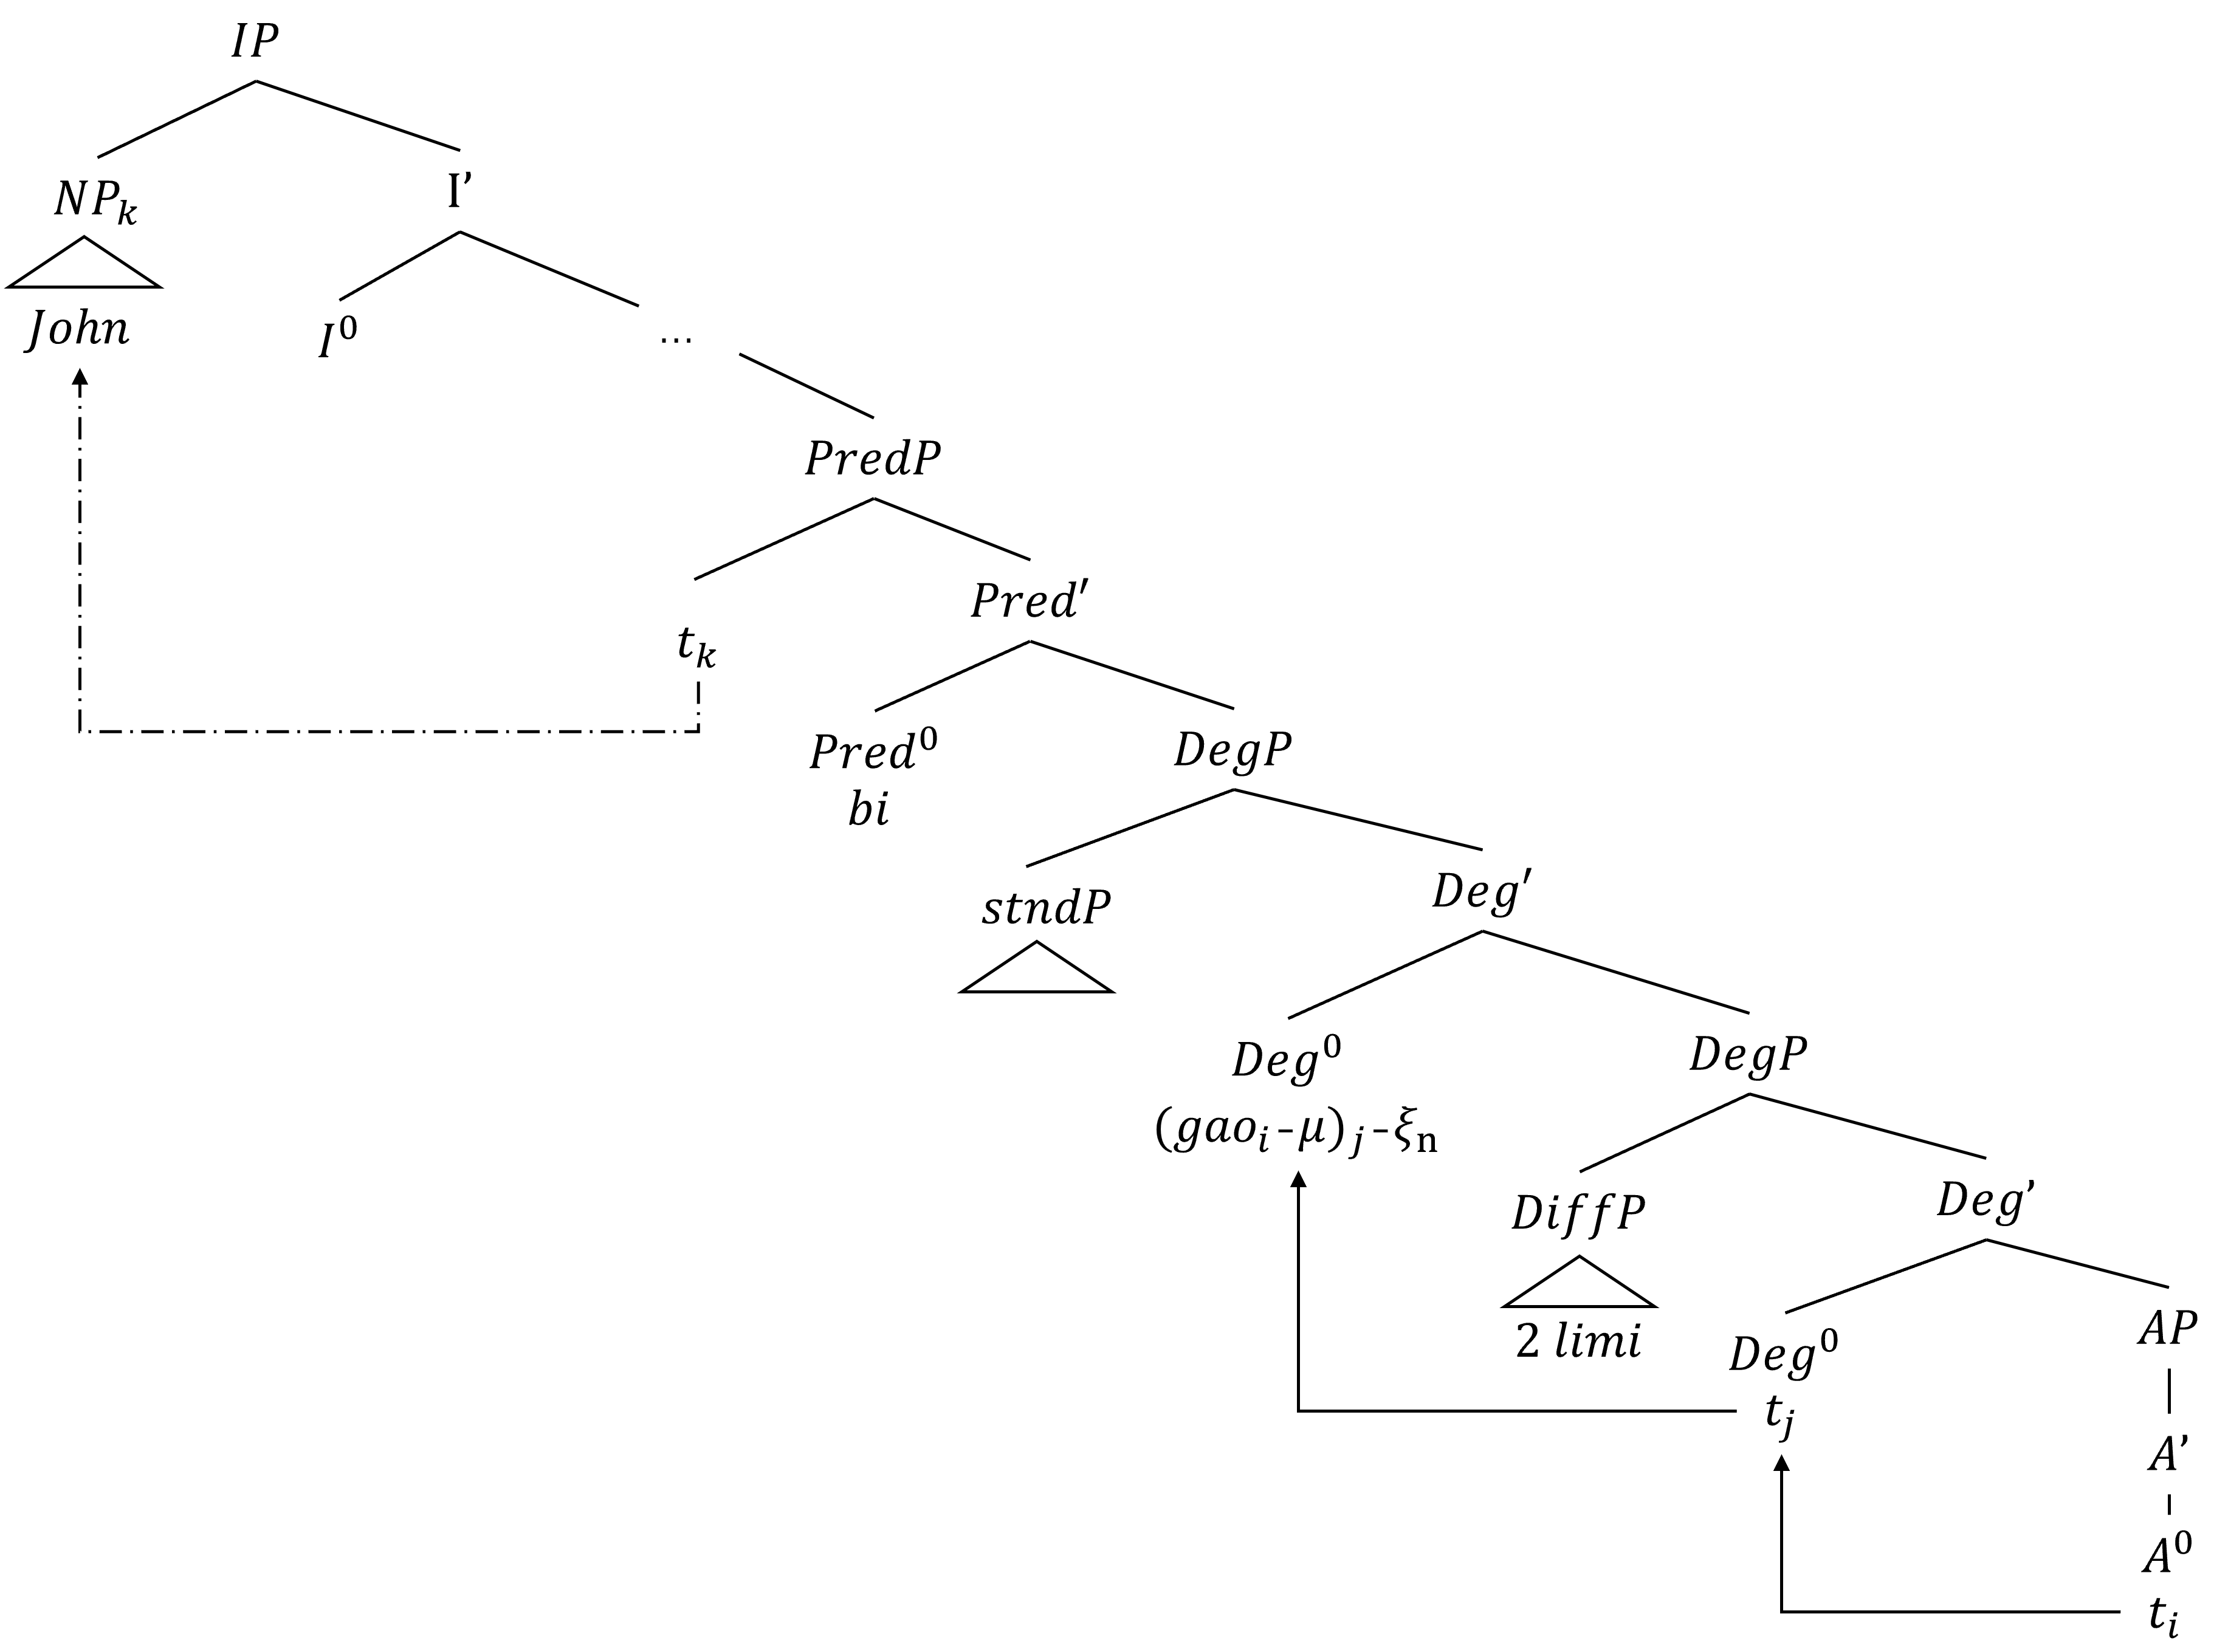
\includegraphics[width=0.8\textwidth]{Pic/superiority_structure_diff.png}
    \begin{caption}
        \\ \vspace{-1.1ex}
        Structure for comparative of superiority with DiffP.
    \end{caption}
\end{figure}

\begin{enumerate}
    \item \label{superiority_example_10}
    \begin{enumerate}
        \item \label{superiority_example_10_a}
        for $\xi_n$, $n=1$ if and only if the standard is a degree;

        \item \label{superiority_example_10_b}
        for $\xi_n$, $n=2$ if and only if the standard is an individual;

        \item \label{superiority_example_10_c}
        for $\xi_n$, $n=3$ if and only if the standard is a set of individuals;

    \end{enumerate}
\end{enumerate}

Continuous head movements are involved. The head of AP first moves upwards to combine with the head of lower DegP, which is instantiated as a null morpheme $\emptyset$ or a bound morpheme with phonetic realization such as \textit{chu}(`exceed'), to form a compound, and then moves together to further combine with the head of the higher DegP when it is instantiated as a bound morpheme. Given that the specifier of PredP is not a position to which Case can be assigned, the comparee denoted by NP(CP) moves to the specifier of TP in order to obtain its Nominative Case.

Like structure of non-DiffP comparative of superiority \ref{superiority_structure}, morpheme \textit{bi}(`than') takes the place of specifier of PredP, which make the building of transitive comparative to be possible. Example in \ref{superiority_example_8_b_transtive} is the transitive version of example \ref{superiority_example_8_b}, in which we can observe that there is no more morpheme \textit{bi}(`than') and the gradable adjective \textit{gao}(`tall') replace the position. The syntactic structure is shown in \ref{superiority_structure_with_DiffP_transitive}. When morpheme \textit{bi}(`than') disappears, the head of PredP becomes null, and the gradable adjective has to be raised up to take this place. 

\begin{enumerate}
    \item \label{superiority_example_8_b_transtive}
    John gao Mary \enspace \enspace \enspace 2limi. \\
    John tall Mary 2 centimeters.  \\
    `John is 2 centimeters taller than Mary.'
\end{enumerate}

\begin{enumerate}
    \item \label{superiority_structure_with_DiffP_transitive}
\end{enumerate}

\begin{figure}[H]
    \centering
    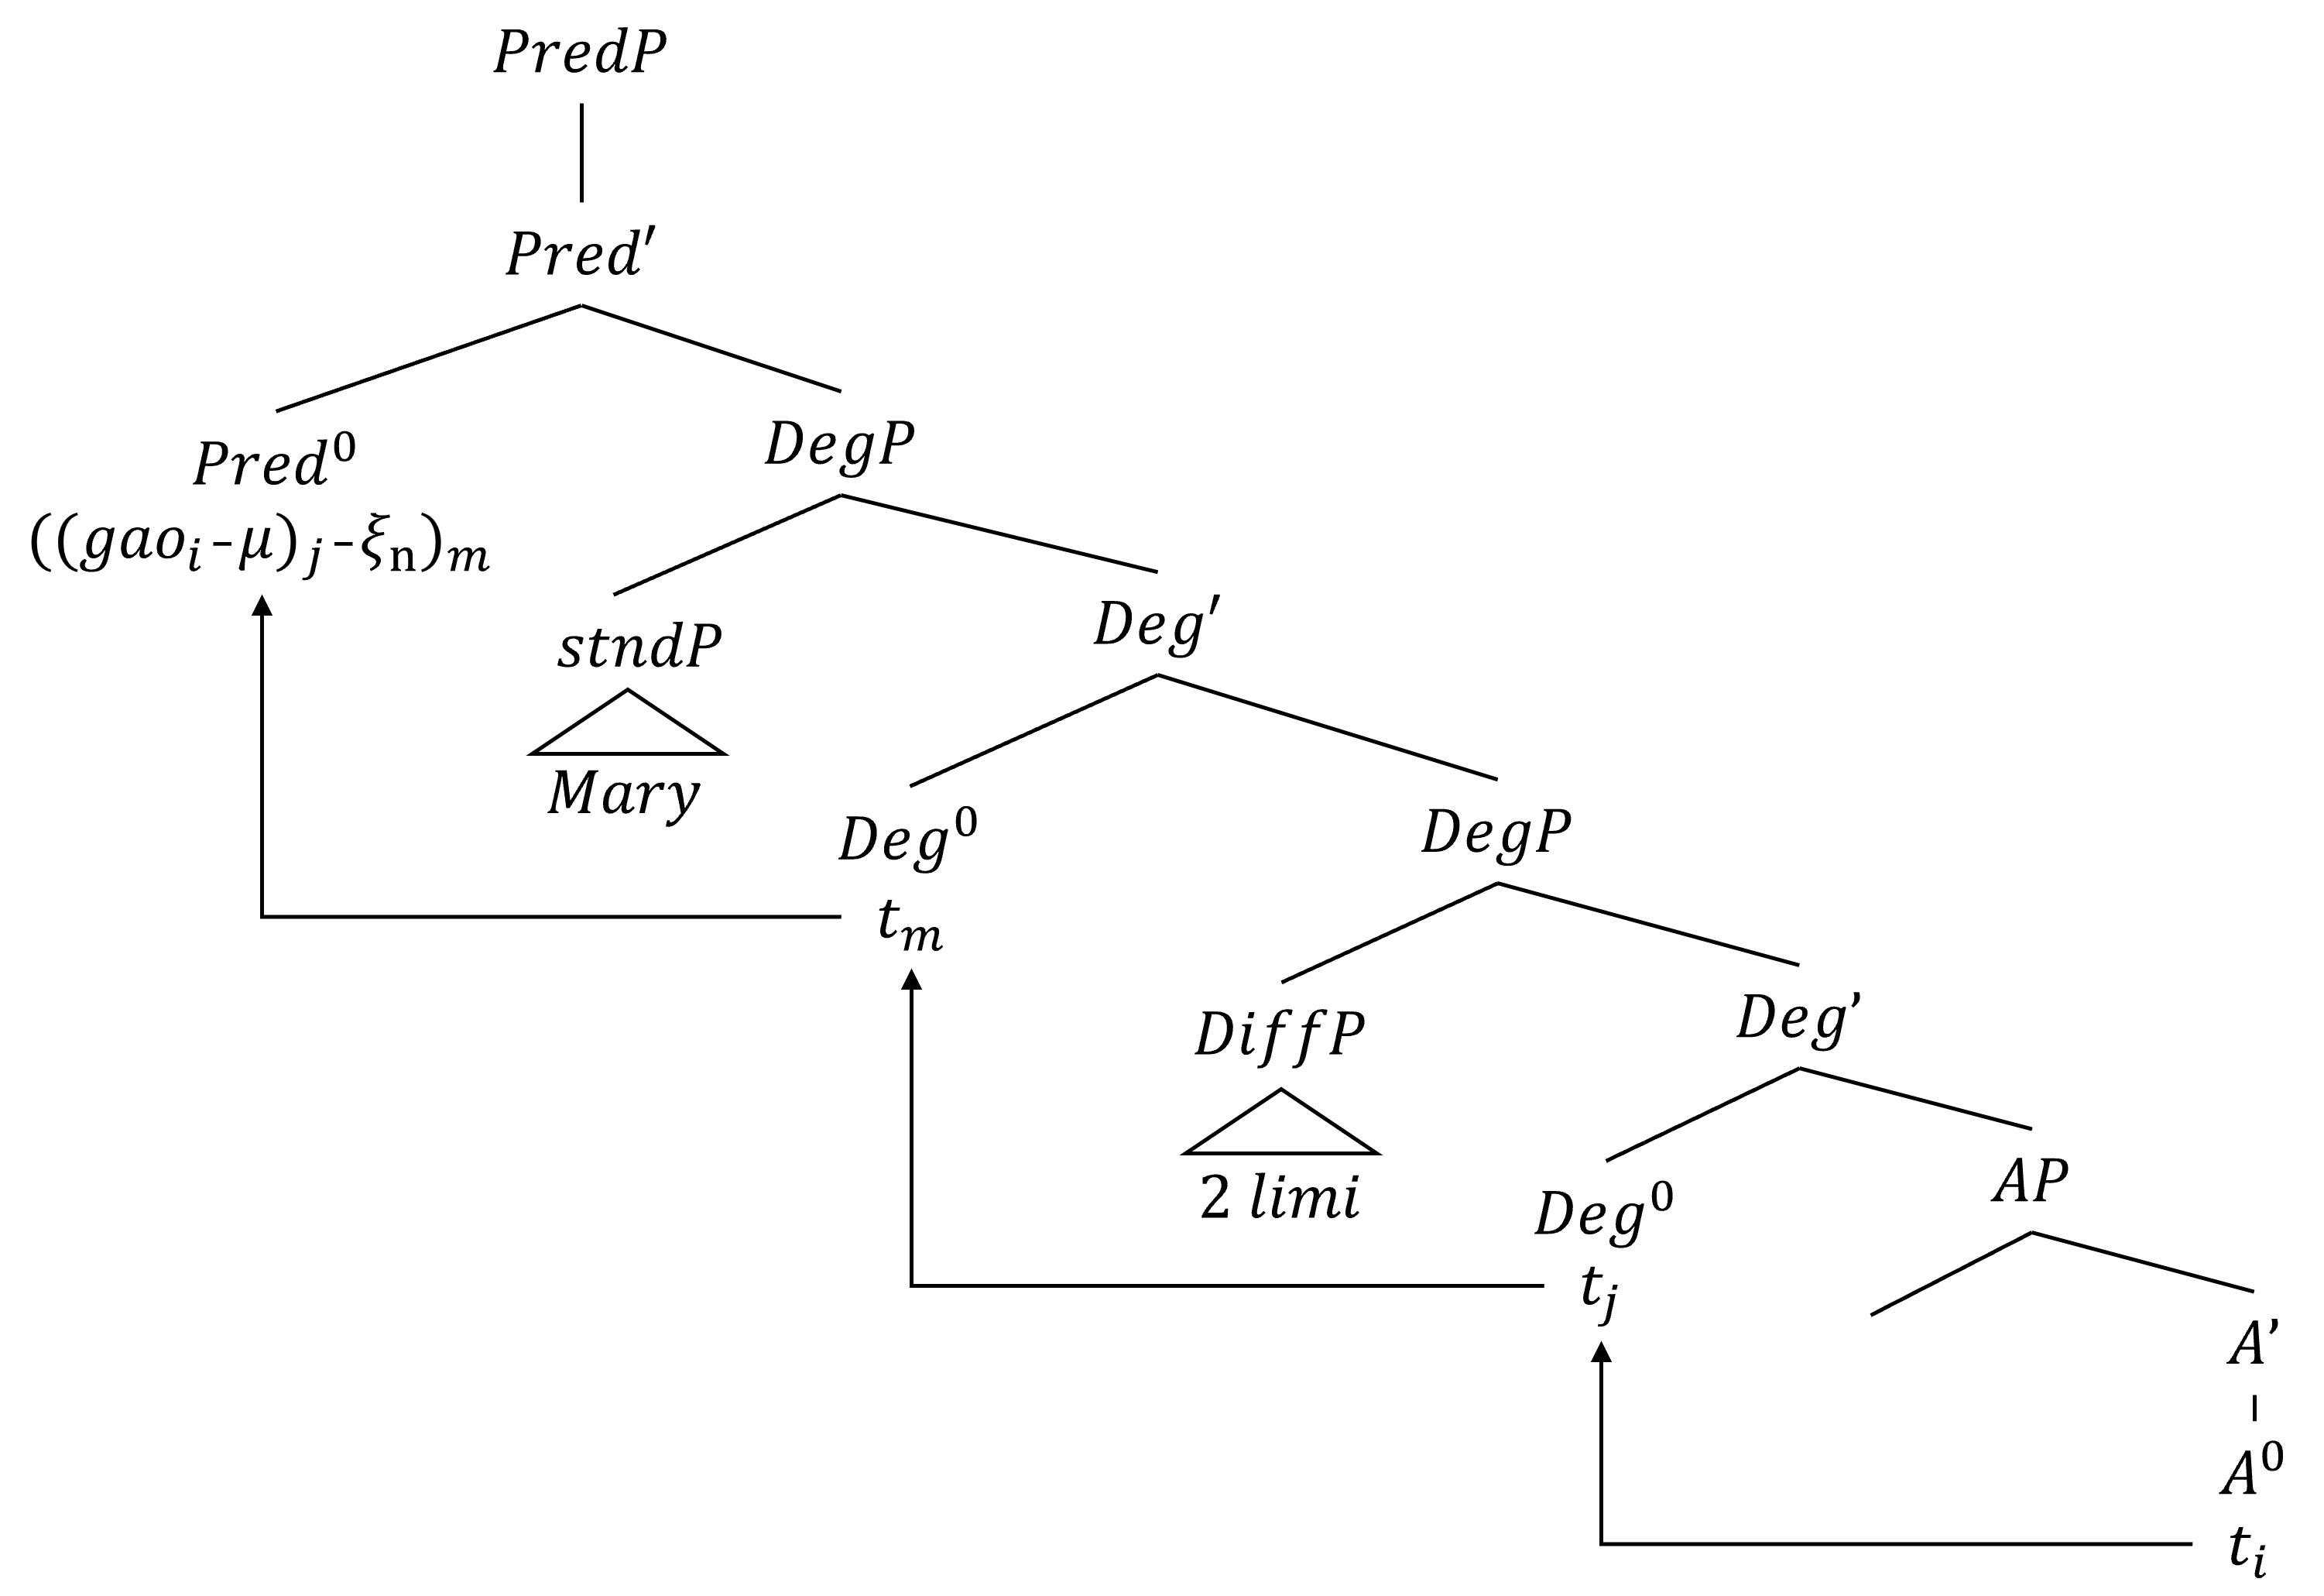
\includegraphics[width=0.7\textwidth]{Pic/superiority_structure_diff_transitive.png}
    \begin{caption}
        \\ \vspace{-1.1ex}
        Structure for transitive comparative of superiority with DiffP.
    \end{caption}
\end{figure}

There is an alternative solution which inverse the hierarchy of the lower DegP and AP, which can be briefly represented as ``DegP-AP-DegP'', supported by many scholars \cite{xiang2005,grano2012}. This structure can also derive out the correct linear order of the sentence. which is displayed in \ref{superiority_example_11} (The structure shown in \ref{superiority_example_11} is slightly different from the original version. Here we do not care about unrelated technical details but just focus on the general structure of the hierarchy of the three layers, i.e., two DegPs and one AP), where AP take the lower DegP as its complement.

\begin{enumerate}
    \item \label{superiority_example_11}
    $\begin{aligned}[t]
        [_{IP} [CompareeP] [_{I^{\prime}} I^{0} [_{...} [[_{DegP} [StndP] [_{Deg^{\prime}} \xi [_{AP} [_{A^{\prime}} A^{0}]]]]]]]] \qquad n \in \{1, 2, 3\}
    \end{aligned}$
\end{enumerate}

In spite of the correct linear order derived, Baker and Hale have argued that the direction of head movements in the syntactic structure shown in \ref{superiority_example_11} is actually impossible \cite{baker1988incorporation,hale1993argument}. They claim that a functional head is an incorporated element rather than an incorporating element, giving rise to the impossibility of the movement from a functional degree head to a lexical adjective head. This assertion eliminates the alternative ``DegP-AP-DegP'' solution from a view of lexicon-syntax.

Now let us turn to semantic part of superiority sentences with DiffP. The semantic interpretation of the higher DegP remains the same as that of superiority sentences without DiffP, so we will not illustrate it in detail again. For the lower DegP, in this paper we assume that it undertake the mere function of measuring the difference between the value of the comparee and the value of  the standard along the dimension of scale denoted by the gradable adjective. It should be pointed out that this difference is expressed in the form of the absolute value for the reason that this difference itself indicates no ordering relation between the two values input into the comparative construction.  The ordering relation is encoded in the lexical entry of gradable adjectives,  indicated neither by the head of higher DegP (which serves merely to usher in the standard) nor by the head of lower DegP (which serves merely to introduce the absolute value of the difference between the two values compared). 

Based on above analyses, the lexical entry of the head of lower DegP is displayed in \ref{maomao14}.  It merely serves to calculate the absolute value of the gap denoted by the differential phrase and whether the comparee or the standard is greater is determined by the gradable adjective which is absorbed by the head of lower DegP. If the gradable adjective is a positive one, like \textit{gao}(`tall'), which encodes $\geq$ relation in its lexical entry repeated as \ref{maomao15_a}, then the difference between the comparee and the standard is a positive value, as proven in \ref{maomao15}. Otherwise, if the gradable adjective is a negative one, like \textit{ai}(`short'), which encodes $\leq$ relation in its lexical entry repeated as \ref{maomao15_a}, then the difference between the comparee and the standard is a negative value, as proven in \ref{maomao16}. Here we use an antonymous pair of gradable adjective to back our analysis of the lower head of DegP as introducer  of the absolute value of the difference between the comparee and the standard.

\begin{enumerate}
    \item \label{maomao14}
    $\begin{aligned}[t]
        [\![\mu]\!] &= \lambda G_{<d,<e,t>>} \lambda d' \lambda d \lambda x.[G(x,d) \land | G \mbox{-} degree(x) - d | = d'] \\
        & <d,<e,t>,<d,<d,<e,t>>>>
    \end{aligned}$
\end{enumerate}


\begin{enumerate}
    \item \label{maomao15}
    \begin{enumerate}
        \item \label{maomao15_a}
        $\begin{aligned}[t]
            [\![gao]\!] &= \lambda d \lambda x.[height(x) \geq d] \qquad <d,<e,t>>
        \end{aligned}$

        \item \label{maomao15_b}
        $\begin{aligned}[t]
            [\![\mu \enspace gao]\!] &= \lambda d' \lambda d \lambda x.[height(x) \geq d \land |height(x) - d|=d'] \\
            & <d,<d,<e,t>>>
        \end{aligned}$
        
        \item \label{maomao15_c}
        \ref{maomao15_b}
        $\begin{aligned}[t]
            \Leftrightarrow [\![\mu \enspace ai]\!] = \lambda d' \lambda d \lambda x.[height(x)-d=-d'] \qquad <d,<d,<e,t>>>
        \end{aligned}$
    \end{enumerate}
\end{enumerate}

\begin{enumerate}
    \item \label{maomao16}
    \begin{enumerate}
        \item \label{maomao16_a}
        $[\![ai]\!] = \lambda d \lambda x.[height(x) leq d] \qquad <d,<e,t>>$

        \item \label{maomao16_b}
        $\begin{aligned}[t]
            [\![\mu \enspace ai]\!] &= \lambda d' \lambda d \lambda x.[height(x) \leq d \land |height(x) - d|=d'] \\
            & <d,<d,<e,t>>>
        \end{aligned}$
        
        \item \label{maomao16_c}
        \ref{maomao16_b}
        $\begin{aligned}[t]
            \Leftrightarrow [\![\mu \enspace gao]\!] = \lambda d' \lambda d \lambda x.[height(x)-d=-d'] \qquad <d,<d,<e,t>>>
        \end{aligned}$
    \end{enumerate}
\end{enumerate}

Sentences classified as comparatives of superiority with DiffP will be conducted with the complete semantic calculations based on semantic compositionality. We will see our analysis can indeed derive out the correct semantic interpretation.

Firstly, \ref{maomao17_a} is a comparative of superiority with DiffP where the standard \textit{1.7 mi}(`1.7meters') is a degree typed $d$. Procedures of its semantic calculations are shown as \ref{maomao17}. The ultimate formalizations actually indicates that ``the height of John is equal to 1.72 meters'', which is equivalent to the meaning of \ref{maomao17_a}.

\begin{enumerate}
    \item \label{maomao17_a}
    John bi \enspace \enspace 1.7mi \enspace \enspace \enspace \enspace gao \enspace \enspace 2limi. \\
    John than 1.7meters tall 2 centimeters. \\
    `John is 2 centimeters taller than 1.7 meters.'
\end{enumerate}

\begin{enumerate}
    \item \label{maomao17}
    \begin{enumerate}
        \item \label{maomao17_b}
        $\begin{aligned}[t]
            [\![\mu]\!] &= \lambda G_{<d,<e,t>>} \lambda d' \lambda d \lambda x.[G(x,d) \land | G \mbox{-} degree(x) - d | = d'] \\
            & <d,<e,t>,<d,<d,<e,t>>>>
        \end{aligned}$
        
        \item \label{maomao17_c}
        $\begin{aligned}[t]
            [\![\mu \enspace gao]\!] &= \lambda d' \lambda d \lambda x.[height(x) \geq d \land |height(x) - d|=d'] \\
            & <d,<d,<e,t>>>
        \end{aligned}$

        \item \label{maomao17_d}
        $\begin{aligned}[t]
            [\![2limi \enspace \mu \enspace gao]\!] &= [\![\mu \enspace gao]\!](2limi) \\
            &= \lambda d \lambda x. [height(x) - d = 2 limi] \qquad <d,<e,t>>
        \end{aligned}$

        \item \label{maomao17_e}
        $\begin{aligned}[t]
            [\![\xi_1 \enspace 2limi \enspace \mu \enspace gao]\!] &= [\![\xi_1]\!]([\![2limi \enspace \mu \enspace gao]\!]) \\
            &= \lambda G_{<d,<e,t>>} \lambda d \lambda x. [G(x,d)](\lambda d' \lambda x'. [height(x') - d' = 2 limi])\\
            &= \lambda d \lambda x. [height(x)-d=2limi] \qquad <d,<e,t>>
        \end{aligned}$

        \item \label{maomao17_f}
        $\begin{aligned}[t]
            [\![1.7mi \enspace \xi_1 \enspace 2limi \enspace \mu \enspace gao]\!] &= [\![\xi_1 \enspace 2limi \enspace \mu \enspace gao]\!](1.7mi) \\
            &=\lambda x.[height(x) -1.7mi=2limi] \qquad <e,t>
        \end{aligned}$

        \item \label{maomao17_g}
        $\begin{aligned}[t]
            [\![John \enspace bi \enspace 1.7mi \enspace \xi_1 \enspace 2limi \enspace \mu \enspace gao]\!] &= [\![1.7mi \enspace \xi_1 \enspace 2limi \enspace \mu \enspace gao]\!](John) \\
            &=height(John) -1.7mi=2limi
        \end{aligned}$

    \end{enumerate}
\end{enumerate}

Secondly, \ref{maomao18_a} is a comparative of superiority with DiffP where the standard \textit{Mary} is an individual typed $e$. Procedures of its semantic calculations are shown as \ref{maomao18}, where similar procedures are not repeated again. In contrast with the formalizations of \ref{maomao_2_13_g} where the wrong semantic interpretation which allows the possibility ``John's height exceeds Mary's height plus 2 centimeters'' derived out via von Stechow's analysis, the ultimate formalizations given in \ref{maomao18_e} via our analysis successfully captures the real meaning of \ref{maomao18_a} that ``John is exactly 2 centimeters taller than Mary''.

\begin{enumerate}
    \item \label{maomao18_a}
    John bi \enspace \enspace Mary gao \enspace \enspace \enspace \enspace 2limi. \\
    John than Mary tall 2 centimeters. \\
    `John is 2 centimeters taller than Mary.'
\end{enumerate}

\begin{enumerate}
    \item \label{maomao18}
    \begin{enumerate}
        \item \label{maomao18_b}
        $\begin{aligned}[t]
            [\![2limi \enspace \mu \enspace gao]\!] &= [\![\mu \enspace gao]\!](2limi) \\
            &= \lambda d \lambda x. [height(x) - d = 2 limi] \qquad <d,<e,t>>
        \end{aligned}$

        \item \label{maomao18_c}
        $\begin{aligned}[t]
            [\![\xi_2 \enspace & 2limi \enspace \mu \enspace gao]\!] \\
            &= [\![\xi_2]\!]([\![2limi \enspace \mu \enspace gao]\!]) \\
            &= \lambda G_{<d,<e,t>>} \lambda y \lambda x. [G(x,G \mbox{-} degree(y))](\lambda d' \lambda x'. [height(x') - d' = 2 limi])\\
            &= \lambda y \lambda x. [height(x) - height(y) = 2 limi] \qquad <d,<e,t>>
        \end{aligned}$

        \item \label{maomao18_d}
        $\begin{aligned}[t]
            [\![Mar&y \enspace \xi_2 \enspace 2limi \enspace \mu \enspace gao]\!] \\
            &= [\![\xi_2 \enspace 2limi \enspace \mu \enspace gao]\!](Mary) \\
            &=\lambda x.[height(x) - height(Mary)=2limi] \qquad <e,t>
        \end{aligned}$

        \item \label{maomao18_e}
        $\begin{aligned}[t]
            [\![John \enspace &bi \enspace Mary \enspace \xi_2 \enspace 2limi \enspace \mu \enspace gao]\!] \\
            &= [\![Mary \enspace \xi_2 \enspace 2limi \enspace \mu \enspace gao]\!](John) \\
            &=height(John) - height(Mary) = 2limi
        \end{aligned}$

    \end{enumerate}
\end{enumerate}


Thirdly, \ref{maomao19_a} is a comparative of superiority with DiffP which is build around a negative gradable adjective \textit{ai}(`short'). Procedures of its semantic calculations are shown as \ref{maomao19}, where similar procedures are not detailed. For ease of understanding, an equivalent form of the ultimate formalization of \ref{maomao19_f} is given in \ref{maomao19_g}, which is paraphrased as ``the height of John equals to the height of Mary minus 2 limi''. This formalizations derives out the correct semantic interpretation of the sentence in \ref{maomao19_a}.

\begin{enumerate}
    \item \label{maomao19_a}
    John bi \enspace \enspace Mary \enspace ai \enspace \enspace \enspace \enspace \enspace 2limi. \\
    John than Mary short 2 centimeters. \\
    `John is 2 centimeters shorter than Mary.'
\end{enumerate}

\begin{enumerate}
    \item \label{maomao19}
    \begin{enumerate}
        \item \label{maomao19_b}
        $[\![\mu \enspace ai]\!]=\lambda d' \lambda d \lambda x.[height(x)-d=d'] \quad <d,<d,<e,t>>>$

        \item \label{maomao19_c}
        $\begin{aligned}[t]
            [\![2limi \enspace \mu \enspace ai]\!] &= [\![\mu \enspace ai]\!](2limi) \\
            &= \lambda d \lambda x. [height(x) - d = -2 limi] \qquad <d,<e,t>>
        \end{aligned}$

        \item \label{maomao19_d}
        $\begin{aligned}[t]
            [\![\xi_2 \enspace & 2limi \enspace \mu \enspace ai]\!] \\
            &= [\![\xi_2]\!]([\![2limi \enspace \mu \enspace ai]\!]) \\
            &= \lambda G_{<d,<e,t>>} \lambda y \lambda x. [G(x,G \mbox{-} degree(y))](\lambda d' \lambda x'. [height(x') - d' = -2 limi])\\
            &= \lambda y \lambda x. [height(x) - height(y) = -2 limi] \qquad <d,<e,t>>
        \end{aligned}$

        \item \label{maomao19_e}
        $\begin{aligned}[t]
            [\![Mar&y \enspace \xi_2 \enspace 2limi \enspace \mu \enspace ai]\!] \\
            &= [\![\xi_2 \enspace 2limi \enspace \mu \enspace ai]\!](Mary) \\
            &=\lambda x.[height(x) - height(Mary)=-2limi] \qquad <e,t>
        \end{aligned}$

        \item \label{maomao19_f}
        $\begin{aligned}[t]
            [\![John \enspace &bi \enspace Mary \enspace \xi_2 \enspace 2limi \enspace \mu \enspace ai]\!] \\
            &= [\![Mary \enspace \xi_2 \enspace 2limi \enspace \mu \enspace ai]\!](John) \\
            &=height(John) - height(Mary) = -2limi
        \end{aligned}$

        \item \label{maomao19_g}
        \ref{maomao19_f} $\Leftrightarrow height(John) = height(Mary) - 2limi$

    \end{enumerate}
\end{enumerate}

Fourthly, (20a) is a comparative of superiority with DiffP where the standard \textit{yi ban}(`half') is a set of individual typed $<e,t>$. However, this pattern manifests itself as ungrammatical. To explain the reason, a review of the semantic interpretation of $\xi_3$, which is always instantiated as \textit{zui}(`most'), is necessary. The lexical entry of $\xi_3$ is repeated in (20b). With a close look at the formalizations, we find that it is actually equivalent to (20c) which means ``the comparee is exactly the one owns the highest degree denoted by the gradable adjective among all people in the appointed set including the comparee himself''. Naturally, it can imply (20d), which is paraphrased as ``the difference between the degree  of the standard denoted by the gradable adjective and the highest degree owned by someone in the appointed set is equal to zero''. However, the composition of $\xi_3$ and the lower DegP will give a semantic interpretation contradictory to that of (20d). As shown in (20e), it indicates that the difference between the degree of the standard denoted by the gradable adjective and the highest degree owned by someone in the appointed set, is not equal to zero. Hence, a comparative of superiority with DiffP in the case of the standard is a set of individual typed $<e,t>$, is deemed ungrammatical.

\begin{enumerate}
    \item \label{maomao20_a}
    * John zai \enspace yiban \enspace \enspace zui \enspace gao \enspace \enspace \enspace 2 limi. \\
    \hspace*{0.5em} John in \enspace class.one most tall 2 centimeters. \\
    \hspace*{0.5em} `John is 2 centimeters tallest in class one.'
\end{enumerate}

\begin{enumerate}
    \item \label{maomao20}
    \begin{enumerate}
        \item \label{maomao20_b}
        $\begin{aligned}[t]
            [\![\xi_3]\!] &= \lambda G_{<d,<e,t>>} \lambda C \lambda x. [x \in C \land G(x,Max \enspace v(v=G \mbox{-} degree(z) \land z \in C))] \\
            & <<d,<e,t>>, <<e,t>,<e,t>>>
        \end{aligned}$

        \item \label{maomao20_c}
        \ref{maomao19_f} 
        $\begin{aligned}[t]
            \Leftrightarrow &\lambda G_{<d,<e,t>>} \lambda C \lambda x. [x \in C \\
            & \land G \mbox{-} degree(x)=Max \enspace v(v=G \mbox{-} degree(z) \land z \in C)]
        \end{aligned}$

        \item \label{maomao20_d}
        \ref{maomao19_f} 
        $\begin{aligned}[t]
            \Leftrightarrow &\lambda G_{<d,<e,t>>} \lambda C \lambda x. [x \in C \\
            & \land G \mbox{-} degree(x) - (Max \enspace v(v=G \mbox{-} degree(z) \land z \in C)) = 0]
        \end{aligned}$

        \item \label{maomao20_e}
        * $\begin{aligned}[t]
            &[\![\xi_3 \enspace 2 limi \enspace \mu \enspace gao]\!] = [\![\xi_3]\!]([\![2 limi \enspace \mu \enspace gao]\!]) \\
            &= \lambda G_{<d,<e,t>>}\lambda C \lambda x. [x \in C \\
            &\qquad \land G(x,Max \enspace v(v=G \mbox{-} degree(z) \land z \in C))](\lambda d' \lambda x'.[height(x)-d=2limi]) \\
            &=\lambda C \lambda x.[x \in C \land height(x)-max \enspace v(v=height(z) \land z \in C)=2limi]\\
            & <<e,t>,<e,t>>
        \end{aligned}$

    \end{enumerate}
\end{enumerate}


\subsection{Equality}

\noindent
A simple example of comparative of equality are shown in \ref{equality_example}. What should be noticed again is that, the equality form is kind of comparative meaning under the classification given in the introduction. The gradable adjectives in equality form bear the function of ``comparsion'' rather than ``assignment''. For example, in \ref{equality_example_1}, gradable adjective \textit{gao}(`tall') does not assign the value of \textit{Mary}'s height to \textit{John}'s height, but make difference between the value of \textit{Mary}'s height and \textit{John}'s height, and the morpheme \textit{yiyang}(`same') gives the truth that this difference is equal to zero. Thus the equality form is a kind of comparative meaning.

\begin{enumerate}
    \item \label{equality_example_1}
    John he \enspace Mary yiyang gao. \\
    John and Mary \enspace same tall. \\
    `John is as tall as Mary.'
\end{enumerate}

The comparative of equality only need two layer structure ``DegP-AP'' to finish its syntactic job, and the tree structure is shown in \ref{equality_example_2}. The \textit{he}(`and') phrase (heP) occupies the specifier of DegP, and the morpheme \textit{yiyang}(`same') is free morpheme, which will block the movement of the gradable adjective \textit{gao}(`tall'). The comparee phrase is denoted by NP(DP) which needs to be assigned with Case. However, the specifier of AP is a position where no Case can be assigned. As a result, the comparee phrase moves to the specifier of IP, where it is assigned Nominative Case.

\begin{enumerate}
    \item \label{equality_example_2}
    $ [_{IP} NP [_{I'} I_0[_{...}[_{DegP}stndP[_{Deg'}Deg^0[_{AP}[A^0]]]]]]]$
\end{enumerate}

\begin{figure}[H]
    \centering
    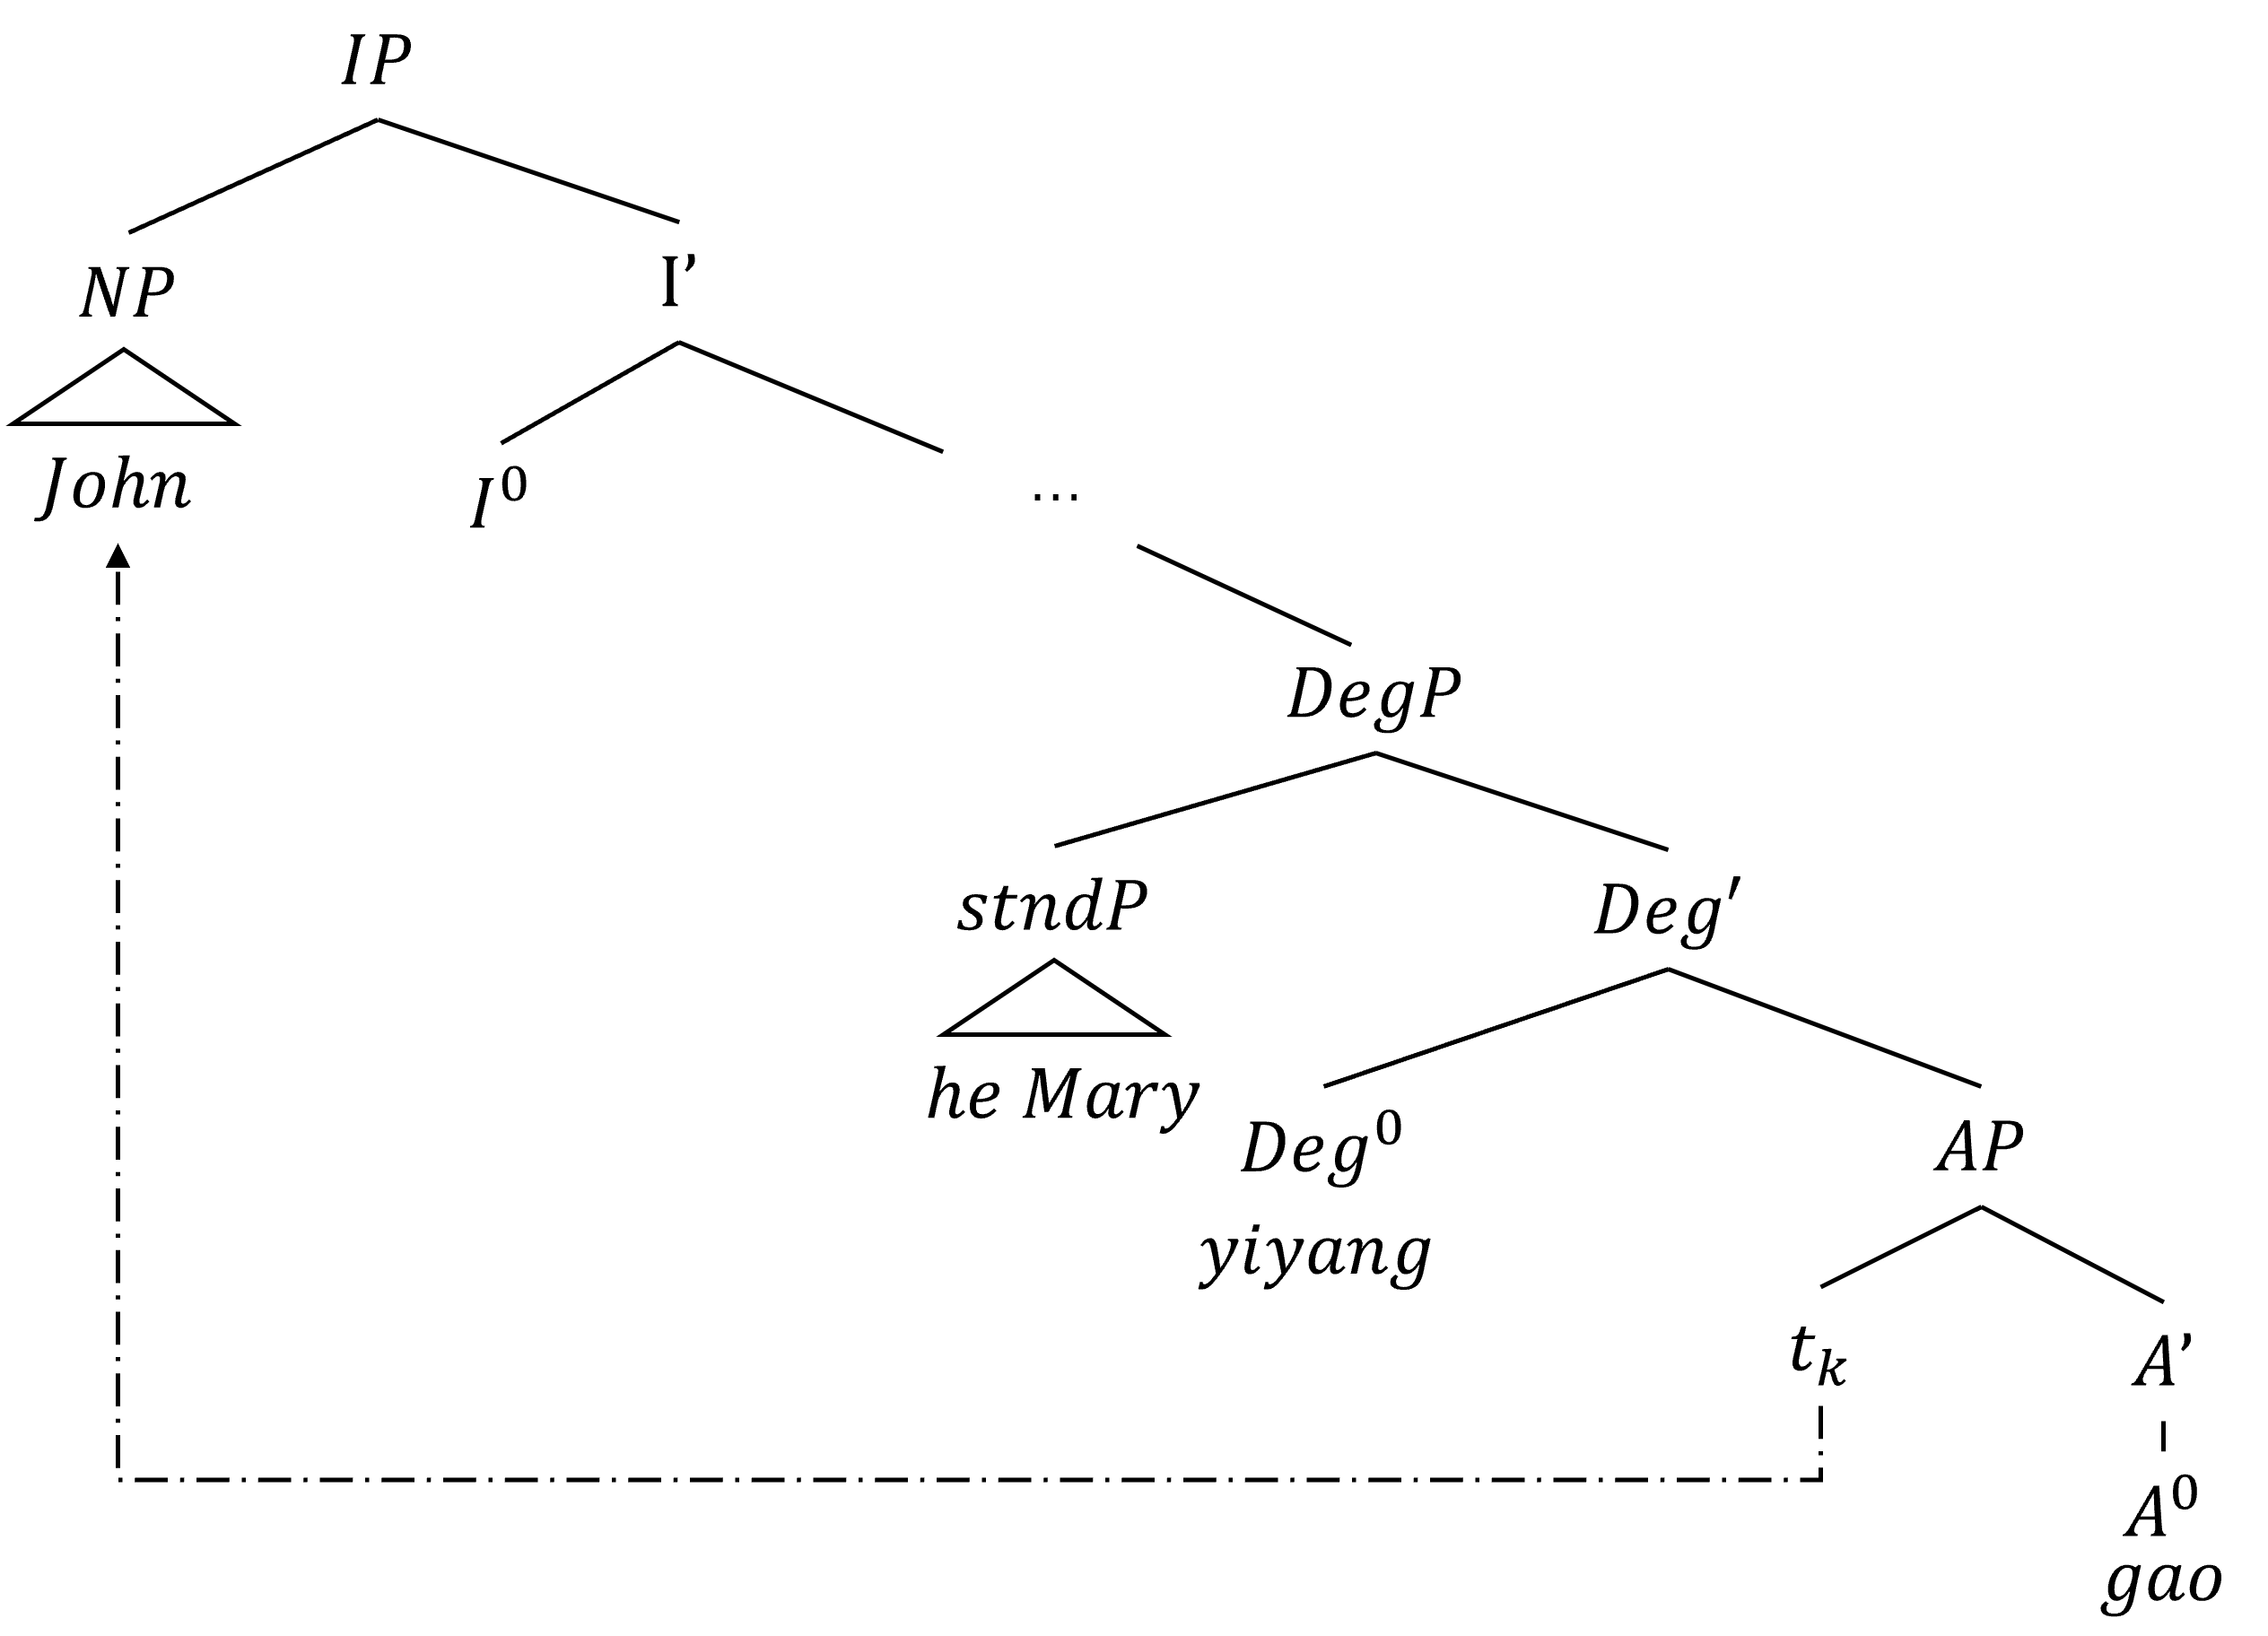
\includegraphics[width=0.5\textwidth]{Pic/yiyanggao.png}
    \begin{caption}
        \\ \vspace{-1.1ex}
        Structure for comparative of positivity.
    \end{caption}
\end{figure}

After syntactic analysis, followed semantic lexical entry calculation. \ref{equality_example_3} is semantic calculation corresponding example \ref{equality_example_1}. The crucial point is the lexical entry of morpheme \textit{yiyang}(`same'), as mentioned above, the essence of comparative of equality is the difference of two values is absolute zero, which is \ref{equality_example_3_a} represent. There is another kine of definition of the lexical entry of \textit{yiyang}(`same') which is shown in \ref{equality_example_3_a_prime}, using equal sign to replace the minus sign. Using this equal sign lexical entry, we can deduce a result which has same expression meaning with \ref{equality_example_3_d}, the reason we do not adopt this is the equal sign always gives a assignment meaning, which is conflict with the comparative meaning.

\begin{enumerate}
    \item \label{equality_example_3}
    \begin{enumerate}
        \item \label{equality_example_3_a}
        $\begin{aligned}[t]
            [\![yiyang]\!] 
            &= \lambda G_{<d,<e,t>>} \lambda y \lambda x.[Max \enspace d_1 G(x,d_1) -  Max \enspace d_2 G(x,d_2) = 0]\\ &
            <<d,<e,t>>,<e,<e,t>>>
        \end{aligned}$

        \item \label{equality_example_3_a_prime}
        $\begin{aligned}[t]
            [\![yiyang_{2}]\!] 
            &= \lambda G_{<d,<e,t>>} \lambda y \lambda x.[Max \enspace d_1 G(x,d_1) =  Max \enspace d_2 G(x,d_2)]\\ &
            <<d,<e,t>>,<e,<e,t>>>
        \end{aligned}$

        \item \label{equality_example_3_b}
        $\begin{aligned}[t]
            [\![yiyang \enspace gao]\!] 
            &= \lambda G_{<d,<e,t>>} \lambda y \lambda x.[Max \enspace d_1 G(x,d_1) - Max \enspace d_2 G(x,d_2) = 0]([\![gao]\!] ) \\
            &= \lambda y \lambda x.[Max \enspace d_1 (height(x) \geq d_1) - Max \enspace d_2 (height(y) \geq d_2) = 0] \\
            & <e,<e,t>>
        \end{aligned}$

        \item \label{equality_example_3_c}
        $\begin{aligned}[t]
            [\![he &\enspace Mary \enspace yiyang \enspace gao]\!] \\
            &= \lambda y \lambda x.[Max \enspace d_1 (height(x) \geq d_1) - Max \enspace d_2 (height(y) \geq d_2) = 0]([\![he \enspace Mary]\!]) \\
            &= \lambda y \lambda x.[Max \enspace d_1 (height(x) \geq d_1) - Max \enspace d_2 (height(y) \geq d_2) = 0](Mary)  \\
            &= \lambda x.[Max \enspace d_1 (height(x) \geq d_1) - Max \enspace d_2 (height(Mary) \geq d_2) = 0] \\
            & <e,t>
        \end{aligned}$

        \item \label{equality_example_3_d}
        $\begin{aligned}[t]
            [\![John &\enspace he \enspace Mary \enspace yiyang \enspace gao]\!] \\
            &= \lambda x.[Max \enspace d_1 (height(x) \geq d_1) - Max \enspace d_2 (height(Mary) \geq d_2) = 0]([\![John]\!]) \\
            &= Max \enspace d_1 (height(John) \geq d_1) - Max \enspace d_2 (height(Mary) \geq d_2) = 0 \\
        \end{aligned}$
    \end{enumerate}
\end{enumerate}

\begin{enumerate}
    \item \label{equality_example_1}
    \begin{enumerate}
        \item \label{equality_example_1_a}
        John he \enspace Mary yiyang gao 2 mi. \\
        John and Mary \enspace same tall 2 meters. \\
        `John is as 2 meters tall as Mary.'

        \item \label{equality_example_1_b}
        John he \enspace Mary yiyang gao \enspace 2 mi \enspace \enspace duo. \\
        John and Mary \enspace same tall 2 meters more. \\
        `John is as more than 2 meters tall as Mary.'
    \end{enumerate}
\end{enumerate}

\section{CONCLUSION}

\noindent
This paper makes a classification to sentences built around gradable predicates in Mandarin by the core semantic interpretation of the gradable adjective. They are generally classified into two main types, i.e., comparative meaning with ``comparison'' function and assignable meaning with ``value assignment'' function. In terms of comparative meaning, this paper further classifies structures into three subtypes, positivity, superiority and equality. Then this paper discusses all these kinds of degree structures from the perspective of generative syntax and formal sematic respectively. 

For the syntactic part, the main contribution of this paper is to assume a flexible as well as clear solution between the selection of ``DegP-AP'' and ``DegP-DegP-AP'' these two syntactic structures. In contrast with the higher DegP undertaking the function to usher in the standard which is projected consistently, the lower DegP undertaking the function to introduce the gap between the comparee and the standard is conditionally projected. Only a differential phrase strictly greater than zero can offer the environment where the lower DegP appears.

For the semantic part, the main contribution of this paper is to make a clear division of labour among the semantic interpretations of the gradable adjective, the lower functional degree head and the higher functional degree head. Semantic formalizations and calculations are illustrated in detail with abundant examples. What's more, some wrong readings which are contradictory to our intuition derived out via previous studies are re-analyzed and corrected under the analysis given in this paper.

\newpage

\printbibliography

\end{document}
